 \documentclass[h]{article}
\usepackage[margin=0.5in]{geometry}
\usepackage{amsfonts} 
\usepackage{textcomp}
 
\usepackage{graphicx}
\usepackage{caption}
\usepackage{subcaption}
\usepackage{float} 
\usepackage{flafter}
\graphicspath{ {../results/vis/} }
\usepackage{adjustbox}


\newcommand{\cent}{\textcent \hspace{4pt}}
\title{CS 7641 Machine Learning \\ Assignment 4}
\date{Due Sunday April 22nd, 2018 11:59pm}
\author{Philip Bale \\ pbale3}

\begin{document}

\maketitle

\section*{Introduction}  
This assignment explores reinforcement learning.  It begins by choosing two 
Markov Decision Procceses (MDPs).  Both MDPs are solved using both value 
iteration and policy iteration, and the results are compared against each other. 
 Afterwards, Q-learning is applied to both problems and those results are then 
 compared to the original results.
 
\subsection*{Problems Chosen}
Gridworld path finding was chosen as the basis for the two Markov Decision Processes.  This 
was done for a few different reasons.  First, the ease in visual representation 
and understanding.  Second, path finding is a common problem in real-life that 
has applications from walking to work, to driving cross-country, etc.  Third, it 
is easy to scale the complexity of a grid as well as increase in the number of 
states.  Fourth, for a solveable grid, one or more optimal solutions must exist. 
 All-in-all, gridworld is great for demonstration reinforcement learning.
 \\ \\ % 30 walls
 The first gridworld problem is an ``easy'' configuration.  It has a 10x10 
 shape with 70 possible states.
% 47 walls
 \\ \\ 
 The second gridworld problem is a ``hard'' configuration.  It has a 20x20 
 shape with 353 possible states.  
 \\ \\
 Each gridworld has its start state is in the bottom left corner and 
 its end state is in the top right corner.  Various ``walls'' exist that force 
 the solution to optimize around.  Various states have negative rewards 
 assosciated with them and are color-coated in the state graphs below.
 
  \begin{figure}[H]
  \minipage{0.05\textwidth}
   \endminipage\hfill
  \minipage{0.45\textwidth}
      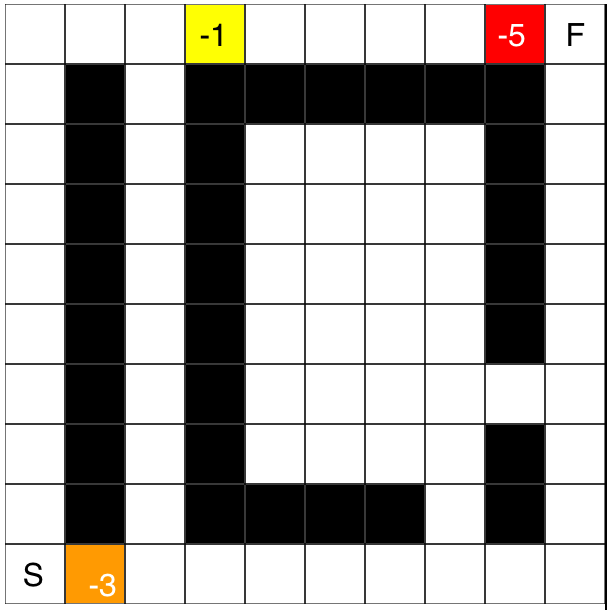
\includegraphics[width=1\textwidth,keepaspectratio]{easy-grid.png} 
      \caption*{10x10 Easy Gridworld w/ 70 States} 
   \endminipage\hfill
   \minipage{0.45\textwidth}
      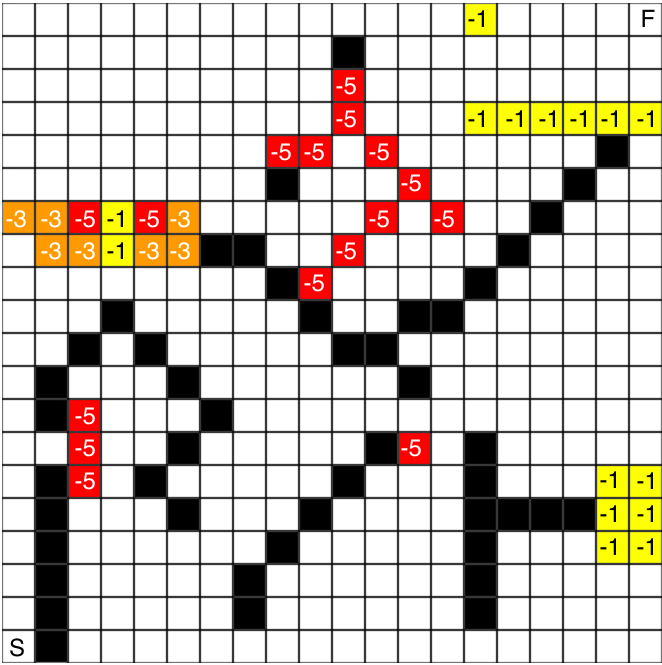
\includegraphics[width=1\textwidth,keepaspectratio]{hard-grid.png} 
      \caption*{20x20 Hard Gridworld w/ 353 States} 
   \endminipage\hfill
   \minipage{0.05\textwidth}
   \endminipage\hfill
\end{figure}


\section*{Value Iteration}
\subsection*{Introduction}
The first reinforcement learning algorithm used to optimally solve the MDPs is Value Iteration. 
 Value iteration works by using the Bellman equation while moving from 
 state to state in an attempt to reach convergence.  Since the utility is not 
 initially known, the algorithm begins with the reward at the final state and works 
 backwards calculating utility for nearest states.  This continues 
 until all states are evaluated.  After a number of iterations, the algorithm 
 will eventually converge on an optimal solution.
 
 
 \begin{figure}[H] 
\centering
\begin{tabular}{ | c | c  | c | c | c | c | c | c| c| c| c| c| c | } 
\hline
\textbf{Iterations} & \textbf{Time} & \textbf{Reward} & \textbf{Steps} & \textbf{Convergence}   \\
\hline
\textbf{EASY Gridworld} \\ \hline
1 & 0.0113 & -199.8800 & 197.4000 & 79.8000 \\ \hline
5 & 0.0545 & -18.6400 & 41.6200 & 20.6322 \\ \hline
10 & 0.1061 & 7.5400 & 24.5000 & 14.1408 \\ \hline
15 & 0.1575 & 34.8000 & 25.4400 & 6.9338 \\ \hline
25 & 0.2520 & 40.9400 & 28.4000 & 1.7116 \\ \hline
35 & 0.2954 & 45.4400 & 48.0800 & 0.0914 \\ \hline
45 & 0.3329 & 47.4400 & 44.5200 & 0.0010 \\ \hline
55 & 0.3735 & 46.0600 & 50.1800 & 2.89e-5 \\ \hline
60 & 0.3931 & 48.4400 & 48.1600 & 3.86e-6 \\ \hline
64 & 0.4090 & 50.0200 & 47.3800 & 8.78e-7 \\ \hline
\\
\textbf{HARD Gridworld} \\ \hline
1 & 0.0501 & -304.6200 & 300 & 83.8968 \\ \hline
5 & 0.1783 & -299 & 300 & 28.6170 \\ \hline
10 & 0.3105 & -299 & 300 & 14.2512 \\ \hline
20 & 0.5473 & -272.1300 & 282.6000 & 4.7330 \\ \hline
25 & 0.6585 & 7.1600 & 64.1800 & 2.7683 \\ \hline
35 & 0.8843 & 13.7700 & 63.4800 & 0.3277 \\ \hline
45 & 1.1318 & 9.1400 & 65.3000 & 0.0054 \\ \hline
55 & 1.3517 & 10.6000 & 63.7800 & 3.16e-5 \\ \hline
61 & 1.4623 & 13.2900 & 62.4400 & 1.72e-6 \\ \hline

\end{tabular}
\caption*{Gridworld Value Iteration Results} 
\end{figure}
 
 \subsubsection*{Easy Gridworld Value Iteration Results}
 The first MDP examined is the easy gridworld pathfinding experiment.  A 10x10 
 grid with various walls, it is a relatively easy problem with a relatively 
 small number of total states.  The results obtained and displayed above lend to various analyses.
 \\ \\
 To measure converge, an iteration threshold of 1e-6 is used.  For this 
 gridworld problem, it takes 64 iterations for value iteration's policy delta to converge 
 below the threshold.  This is reasonable, as the value iteration works 
 backwards and attempts to find the best possible policy.  Improvements are made 
 overtime and eventually it, in this case at 64 iterations, falls below our 
 threshold.    
 \\ \\
 In terms of performance, the maximum reward value is found at iteration \#64--indicating 
 that that value iteration found an optimal policy.  At 64 steps, the journey 
 taken is much more complex than the naive solutions found at iteration \#5.  
 Unsurprisingly, the shortest path is not necessarily the most valuable.  In 
 terms of iteration time, the algorithm is rather fast--less than half of a 
 second to converge on my machine.  Observing the policy maps below, the algorithm does well at determining an optimal policy for the various possible states. 
 
  \subsubsection*{Hard Gridworld Value Iteration Results}
 The second MDP examined is the hard gridworld pathfinding experiment.  A 20x20 
 grid with various walls, it is significantly more complex than the easy 
 gridworld layout--there are many more states, rewards, and walls.
  \\ \\
 Similar to above, to measure converge, an iteration threshold of 1e-6 is used.  For this 
 gridworld problem, it takes 61 iterations for value iteration's policy delta to converge 
 below the threshold.  While a more complex problem than before, it demonstates that problem complexity does not gaurantee 
 that more iterations are necessary for convergence.
 \\ \\
 Performance-wise, the maximum reward is actually not found at the last 
 iteration where convergence is achieved, but rather at iteration \#35.  It 
 does, however, fall within a very small margin of the last iteration \#61.  
 The path of the highest reward solution is approximately 63 
 steps--significantly less than the initial solutions of around 300 steps.  The 
 hard gridworld problem, reasonable, takes signficiantly longer to converge than 
 the easy problem (1.4 seconds vs 0.4).
 Viewing the policy maps below, it becomes clear that the algorithm does a 
 rather superb job at determining a policy with the best action to take at the various states.
 
   \begin{figure}[H]
  \minipage{0.245\textwidth}
      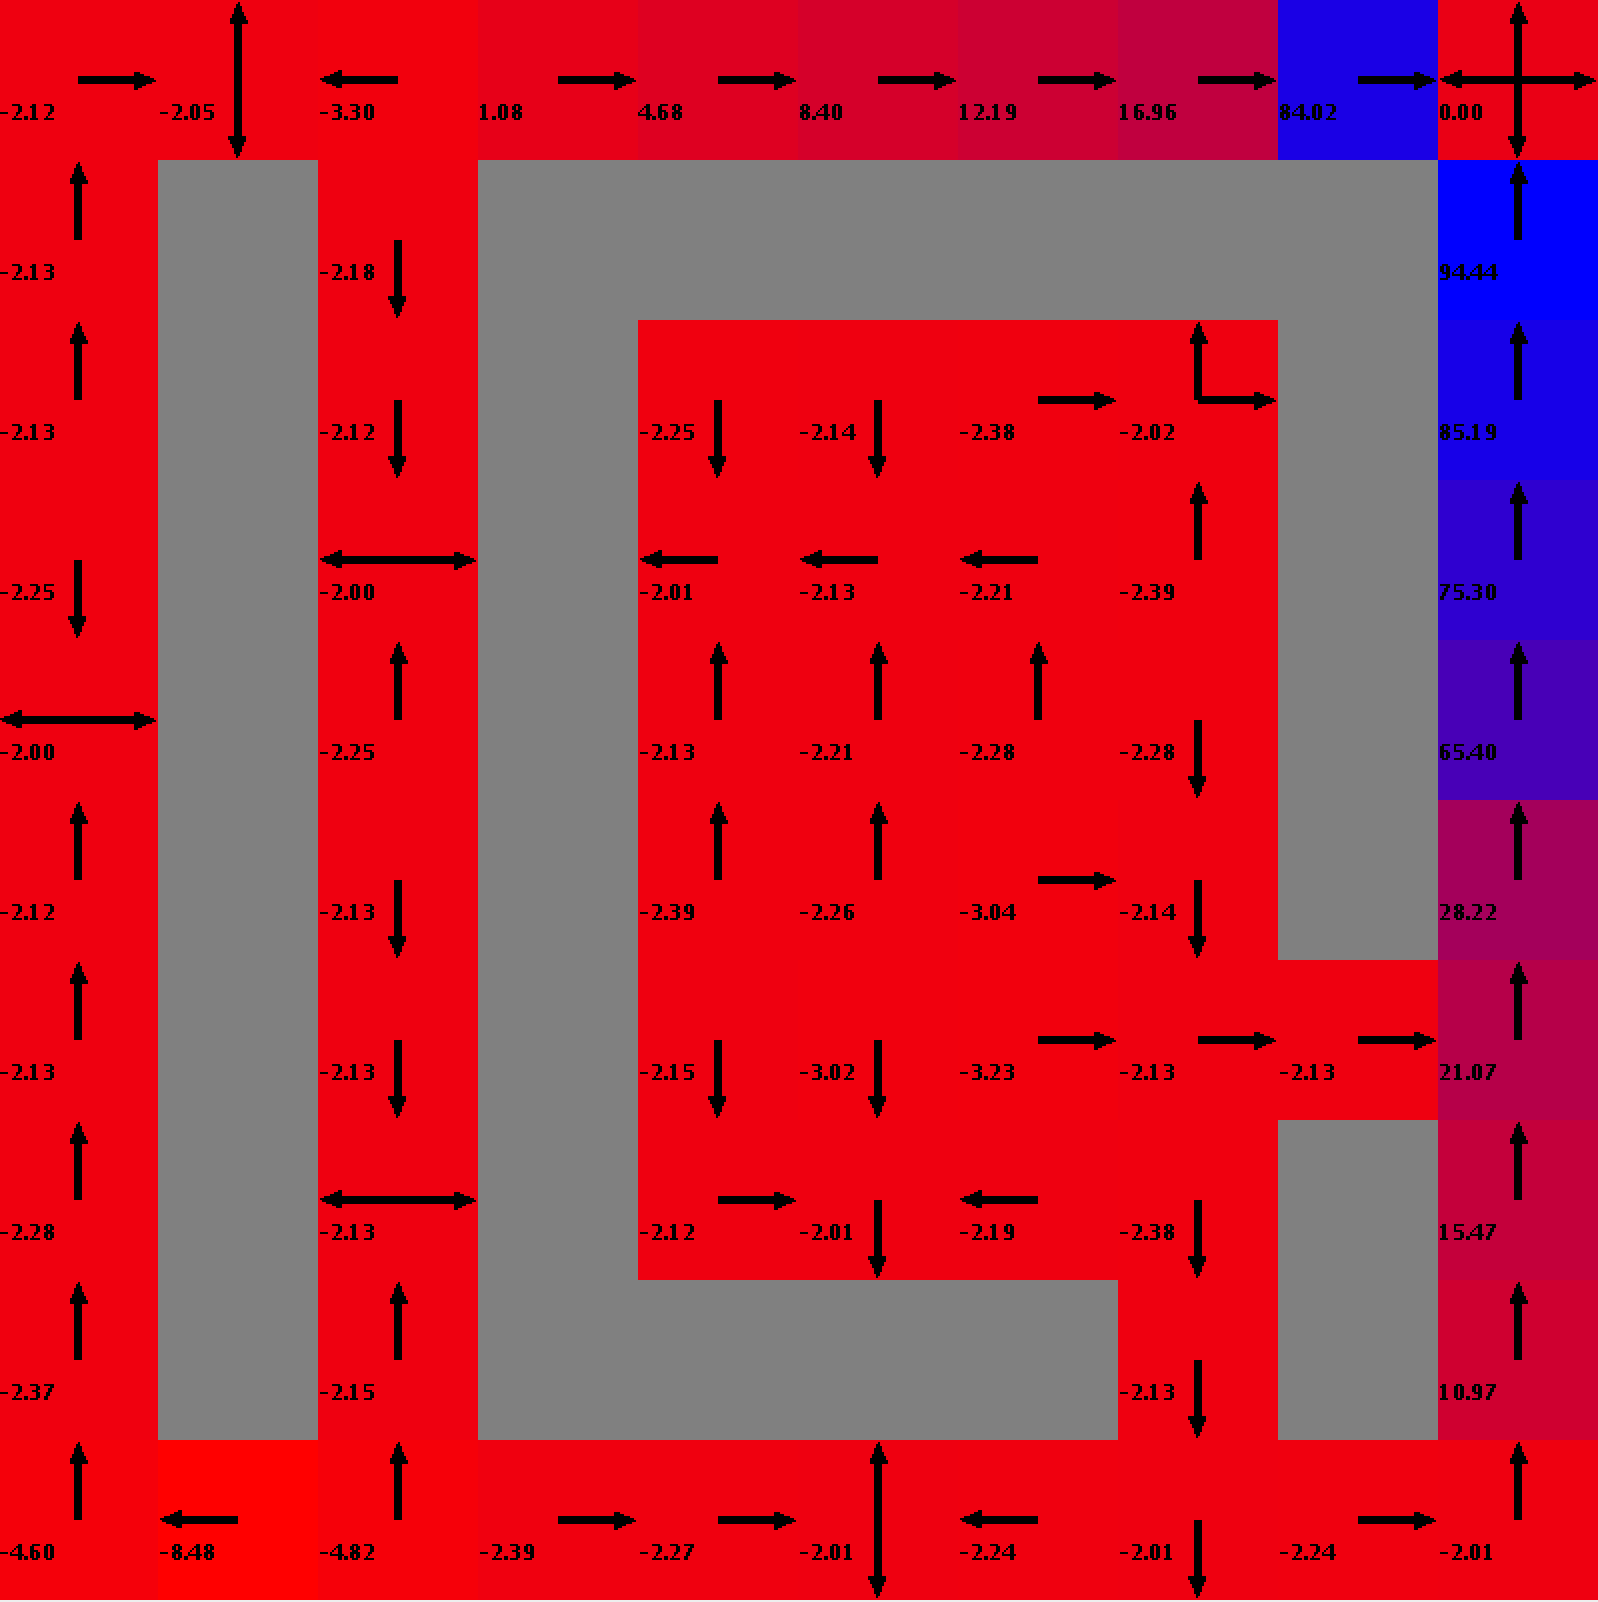
\includegraphics[width=1\textwidth,keepaspectratio]{easy-value-2.png} 
      \caption*{Easy GW Value Iteration \#2} 
   \endminipage\hfill
   \minipage{0.245\textwidth}
      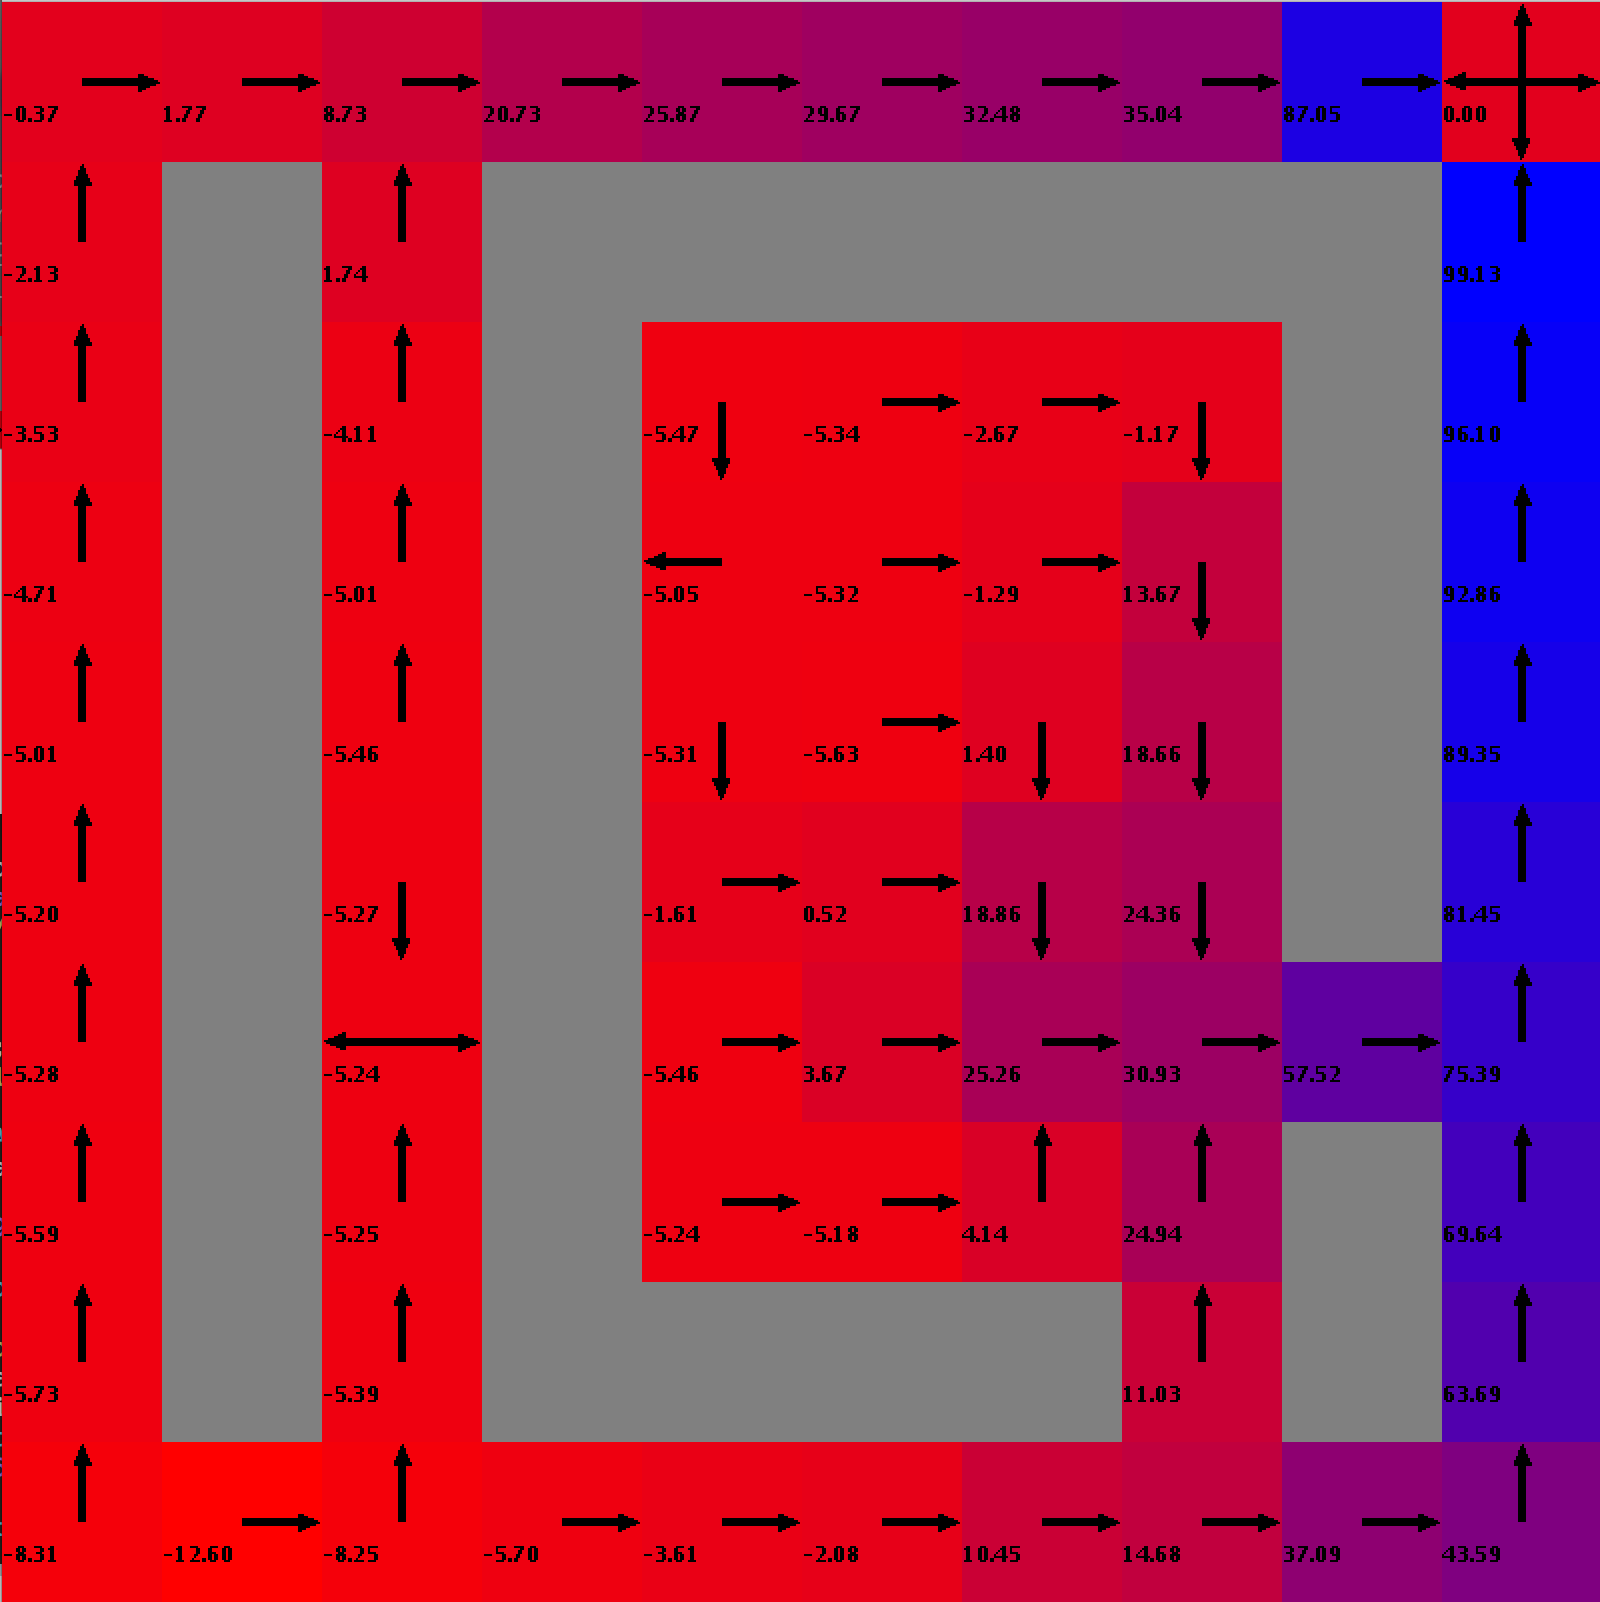
\includegraphics[width=1\textwidth,keepaspectratio]{easy-value-5.png} 
      \caption*{Easy GW Value Iteration \#5} 
   \endminipage\hfill
   \minipage{0.245\textwidth}
      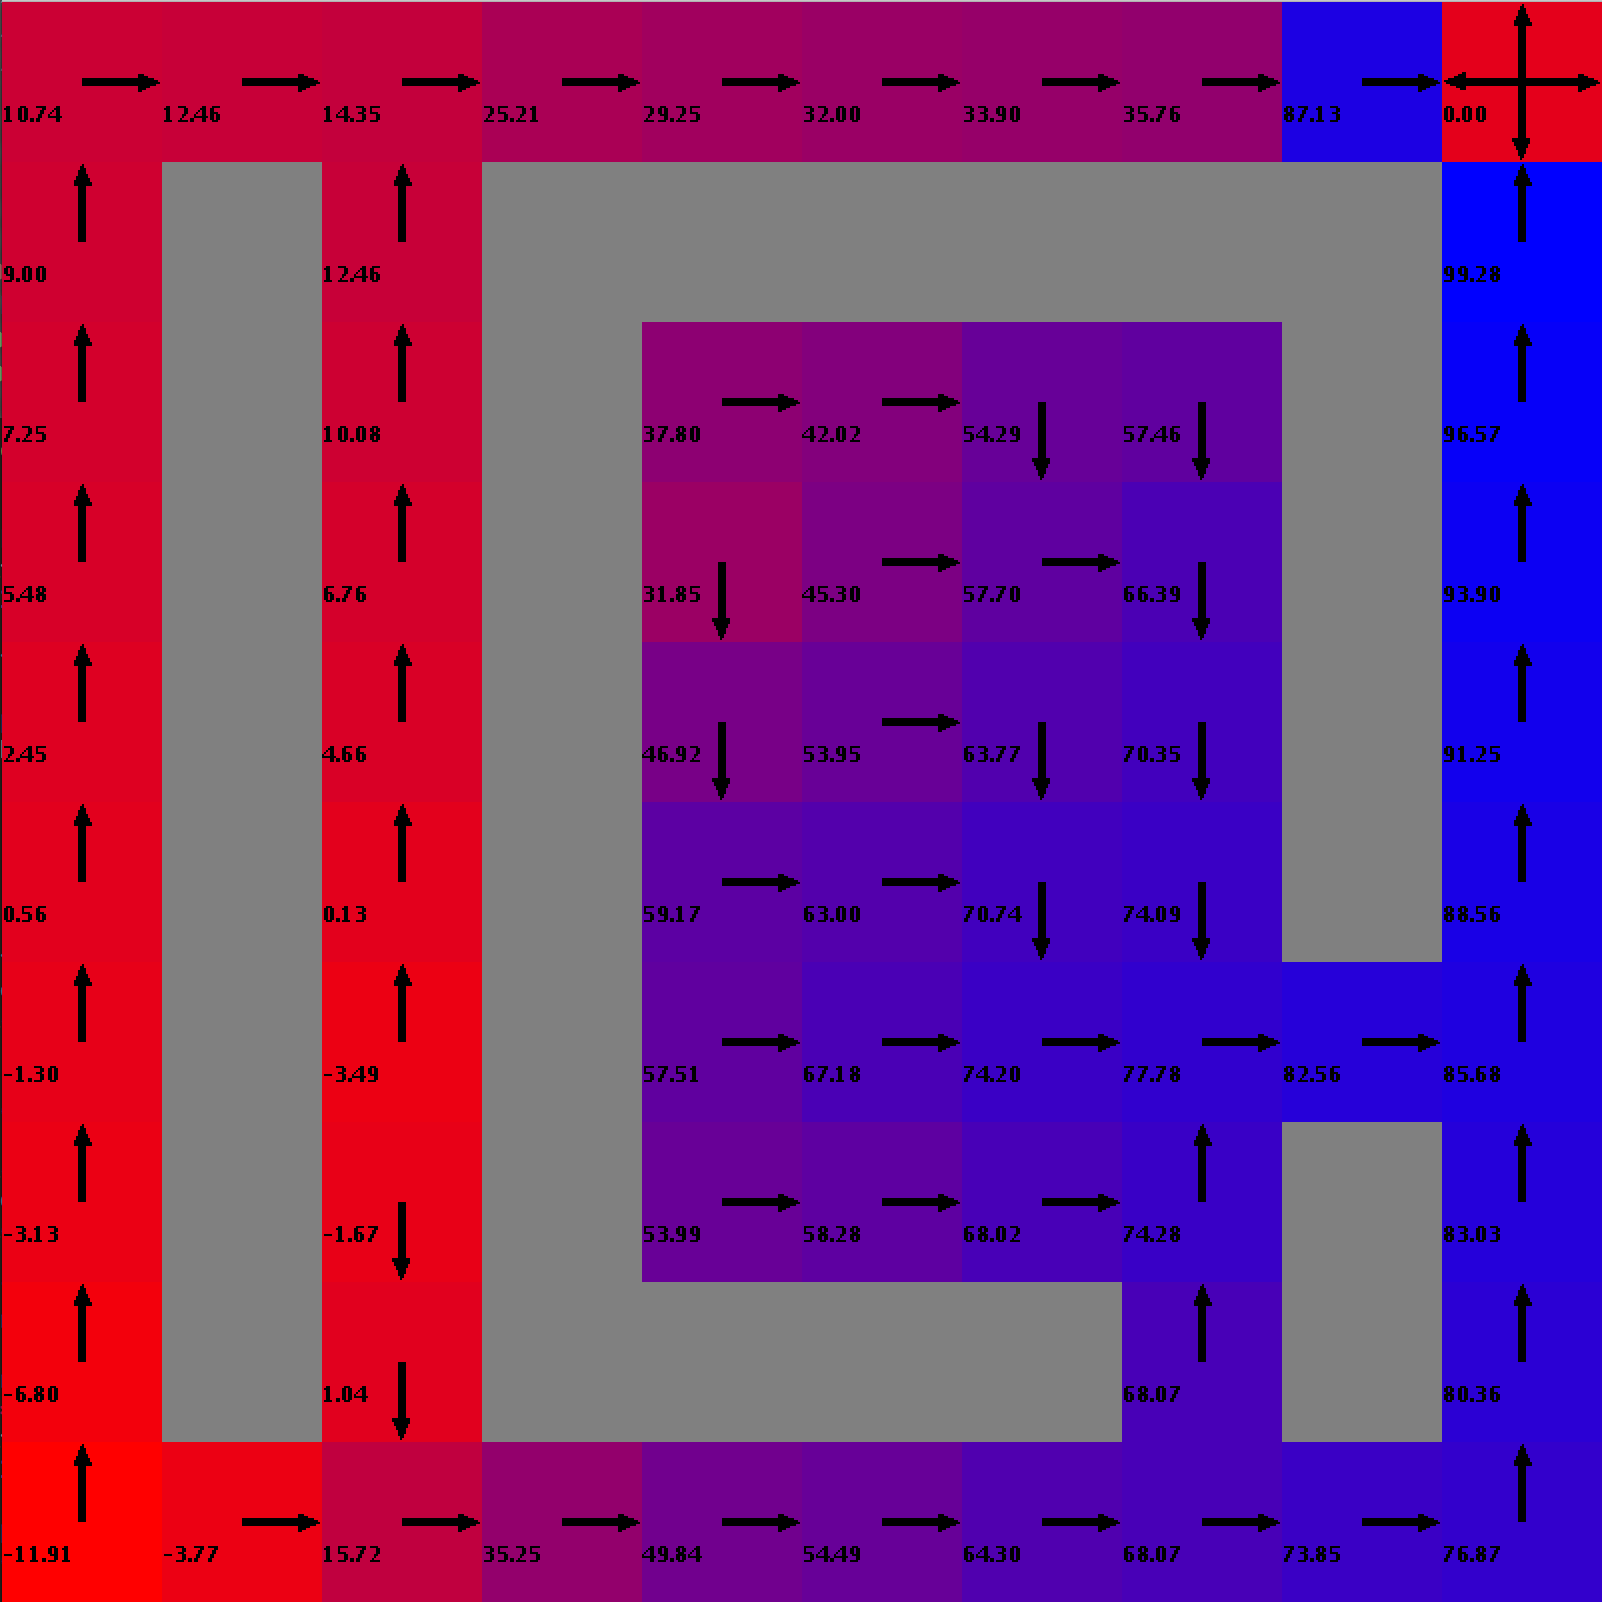
\includegraphics[width=1\textwidth,keepaspectratio]{easy-value-10.png} 
      \caption*{Easy GW Value Iteration \#10} 
   \endminipage\hfill
   \minipage{0.245\textwidth}
      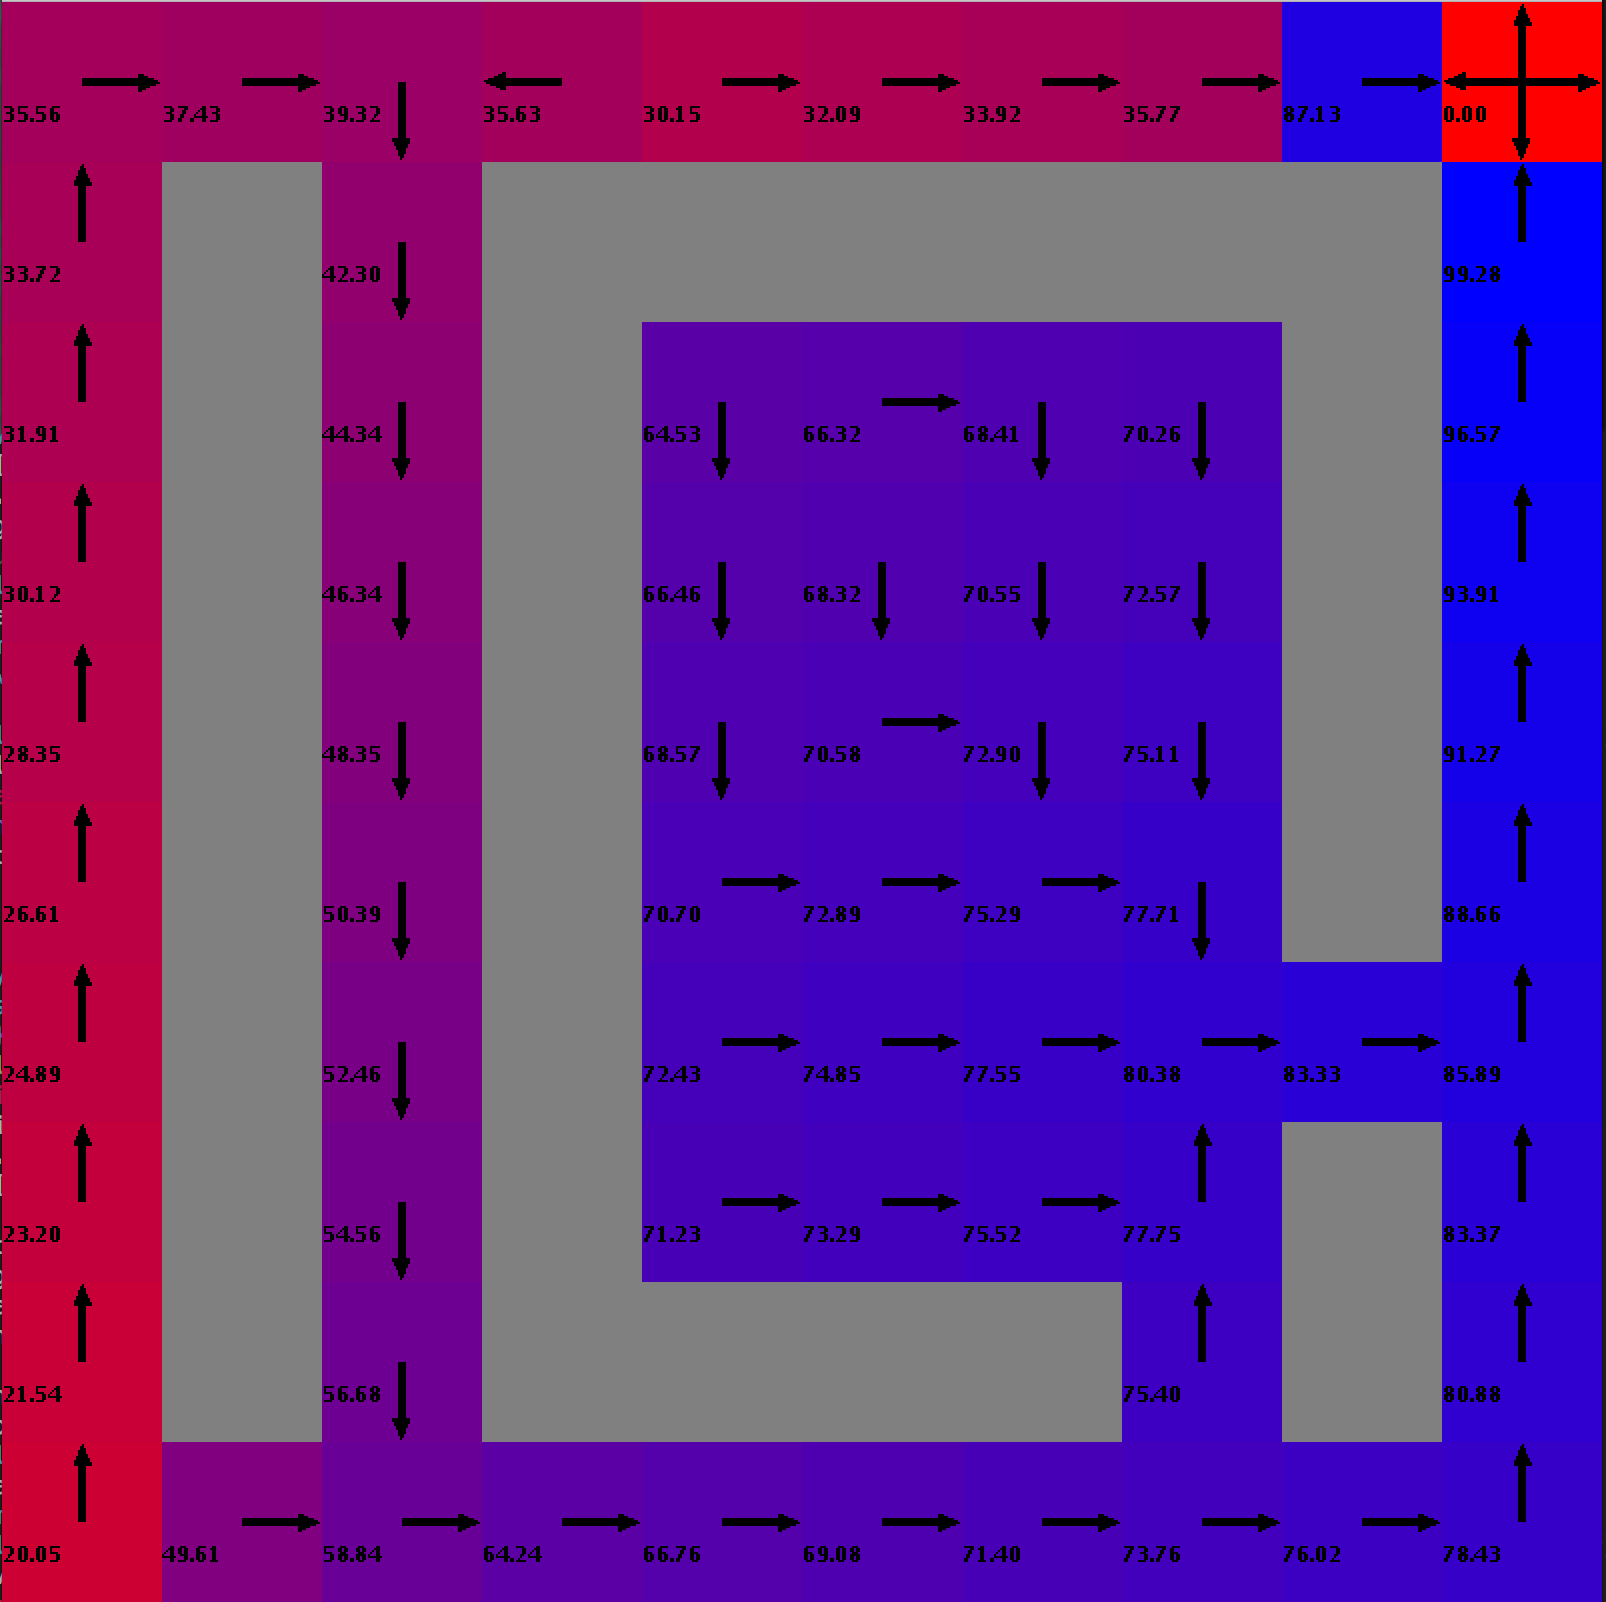
\includegraphics[width=1\textwidth,keepaspectratio]{easy-value-64.png} 
      \caption*{Easy GW Value Iteration \#64} 
   \endminipage\hfill
\end{figure}


   \begin{figure}[H]
  \minipage{0.245\textwidth}
      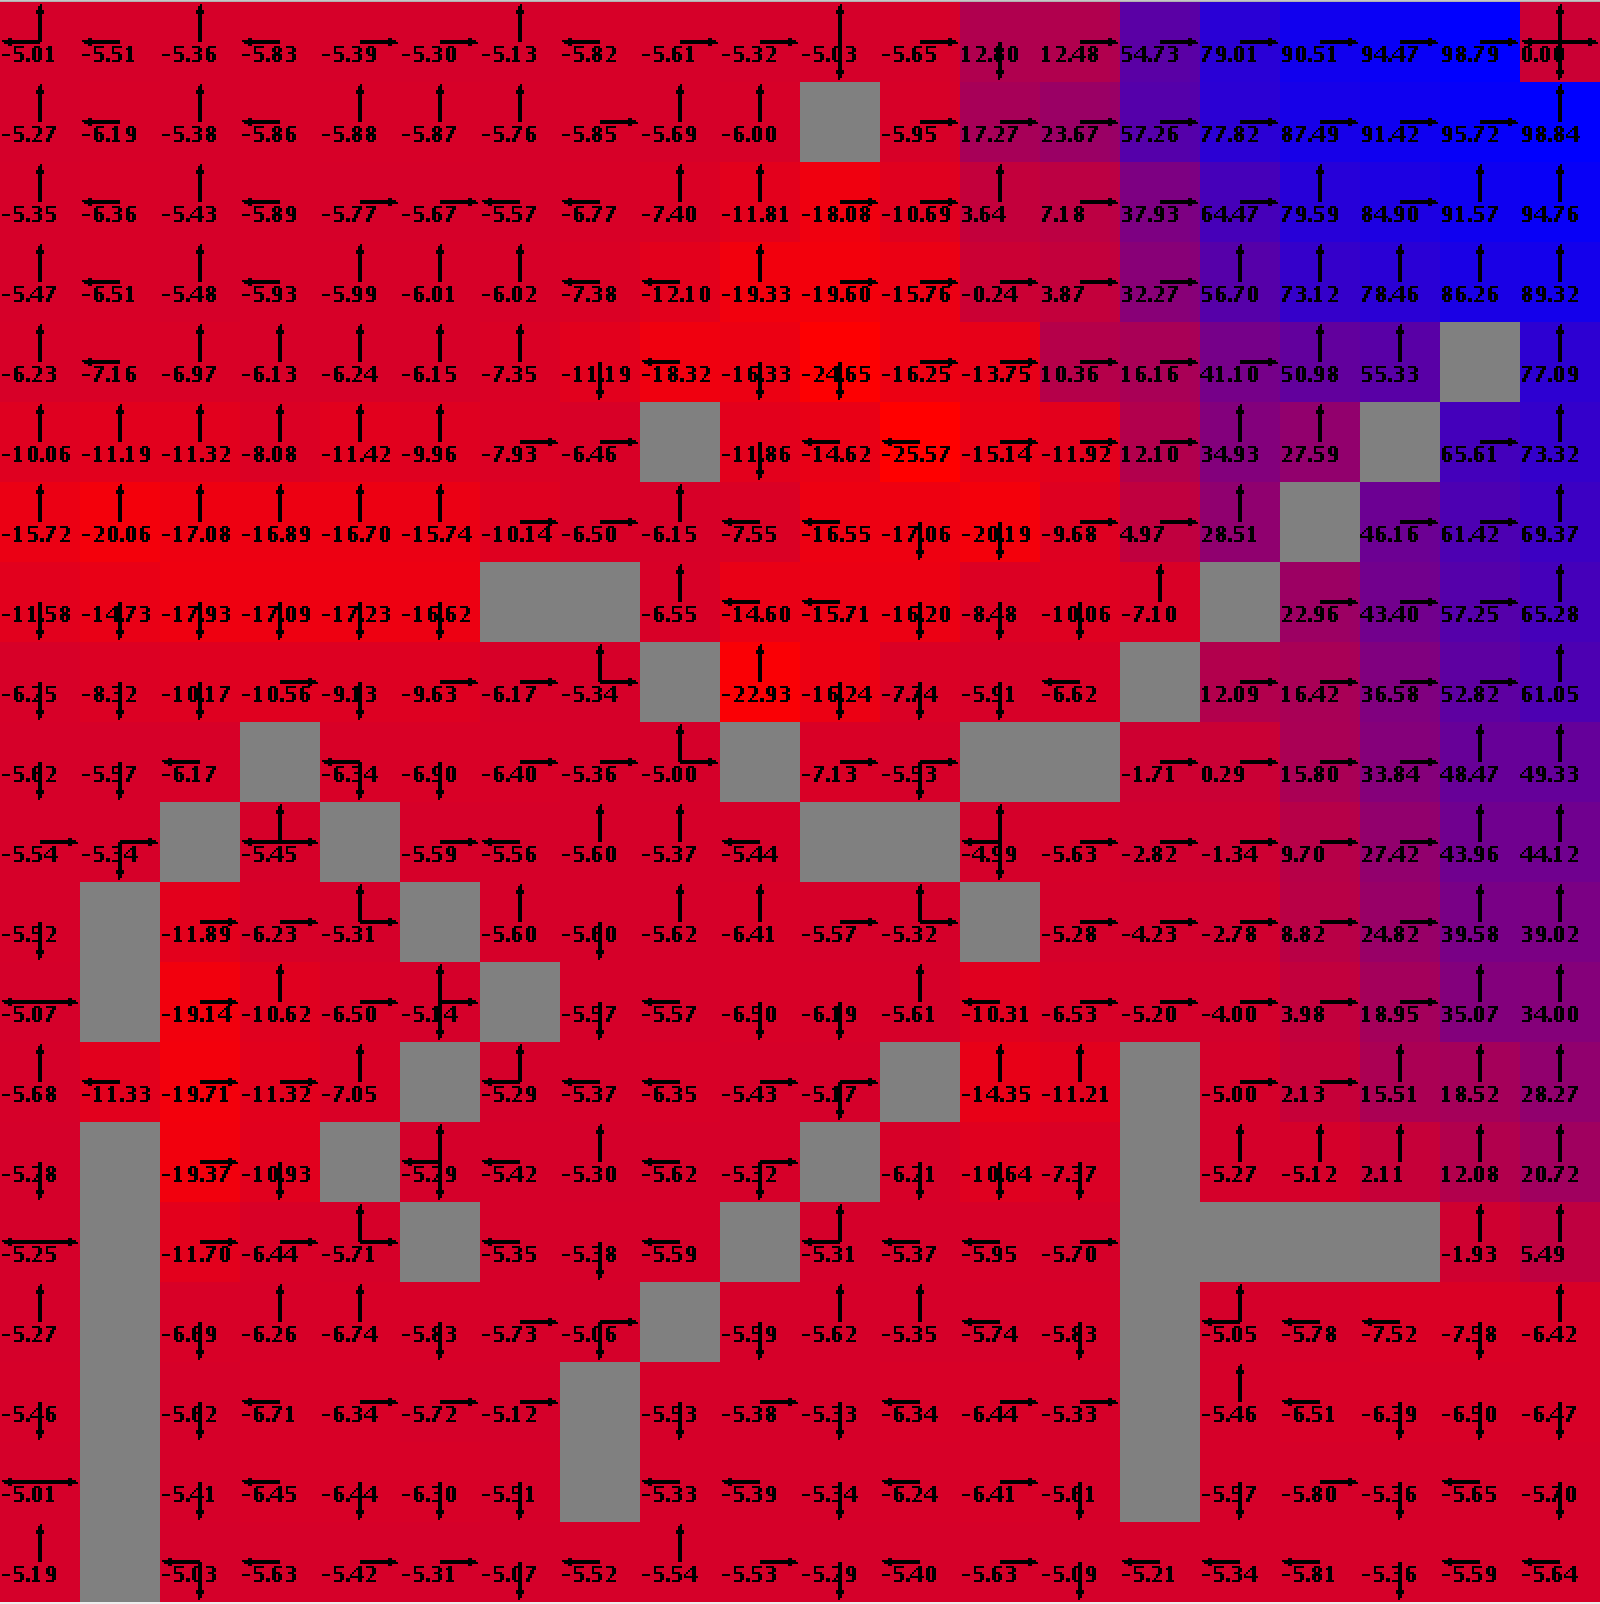
\includegraphics[width=1\textwidth,keepaspectratio]{hard-value-5.png} 
      \caption*{Hard GW Value Iteration \#5} 
   \endminipage\hfill
   \minipage{0.245\textwidth}
      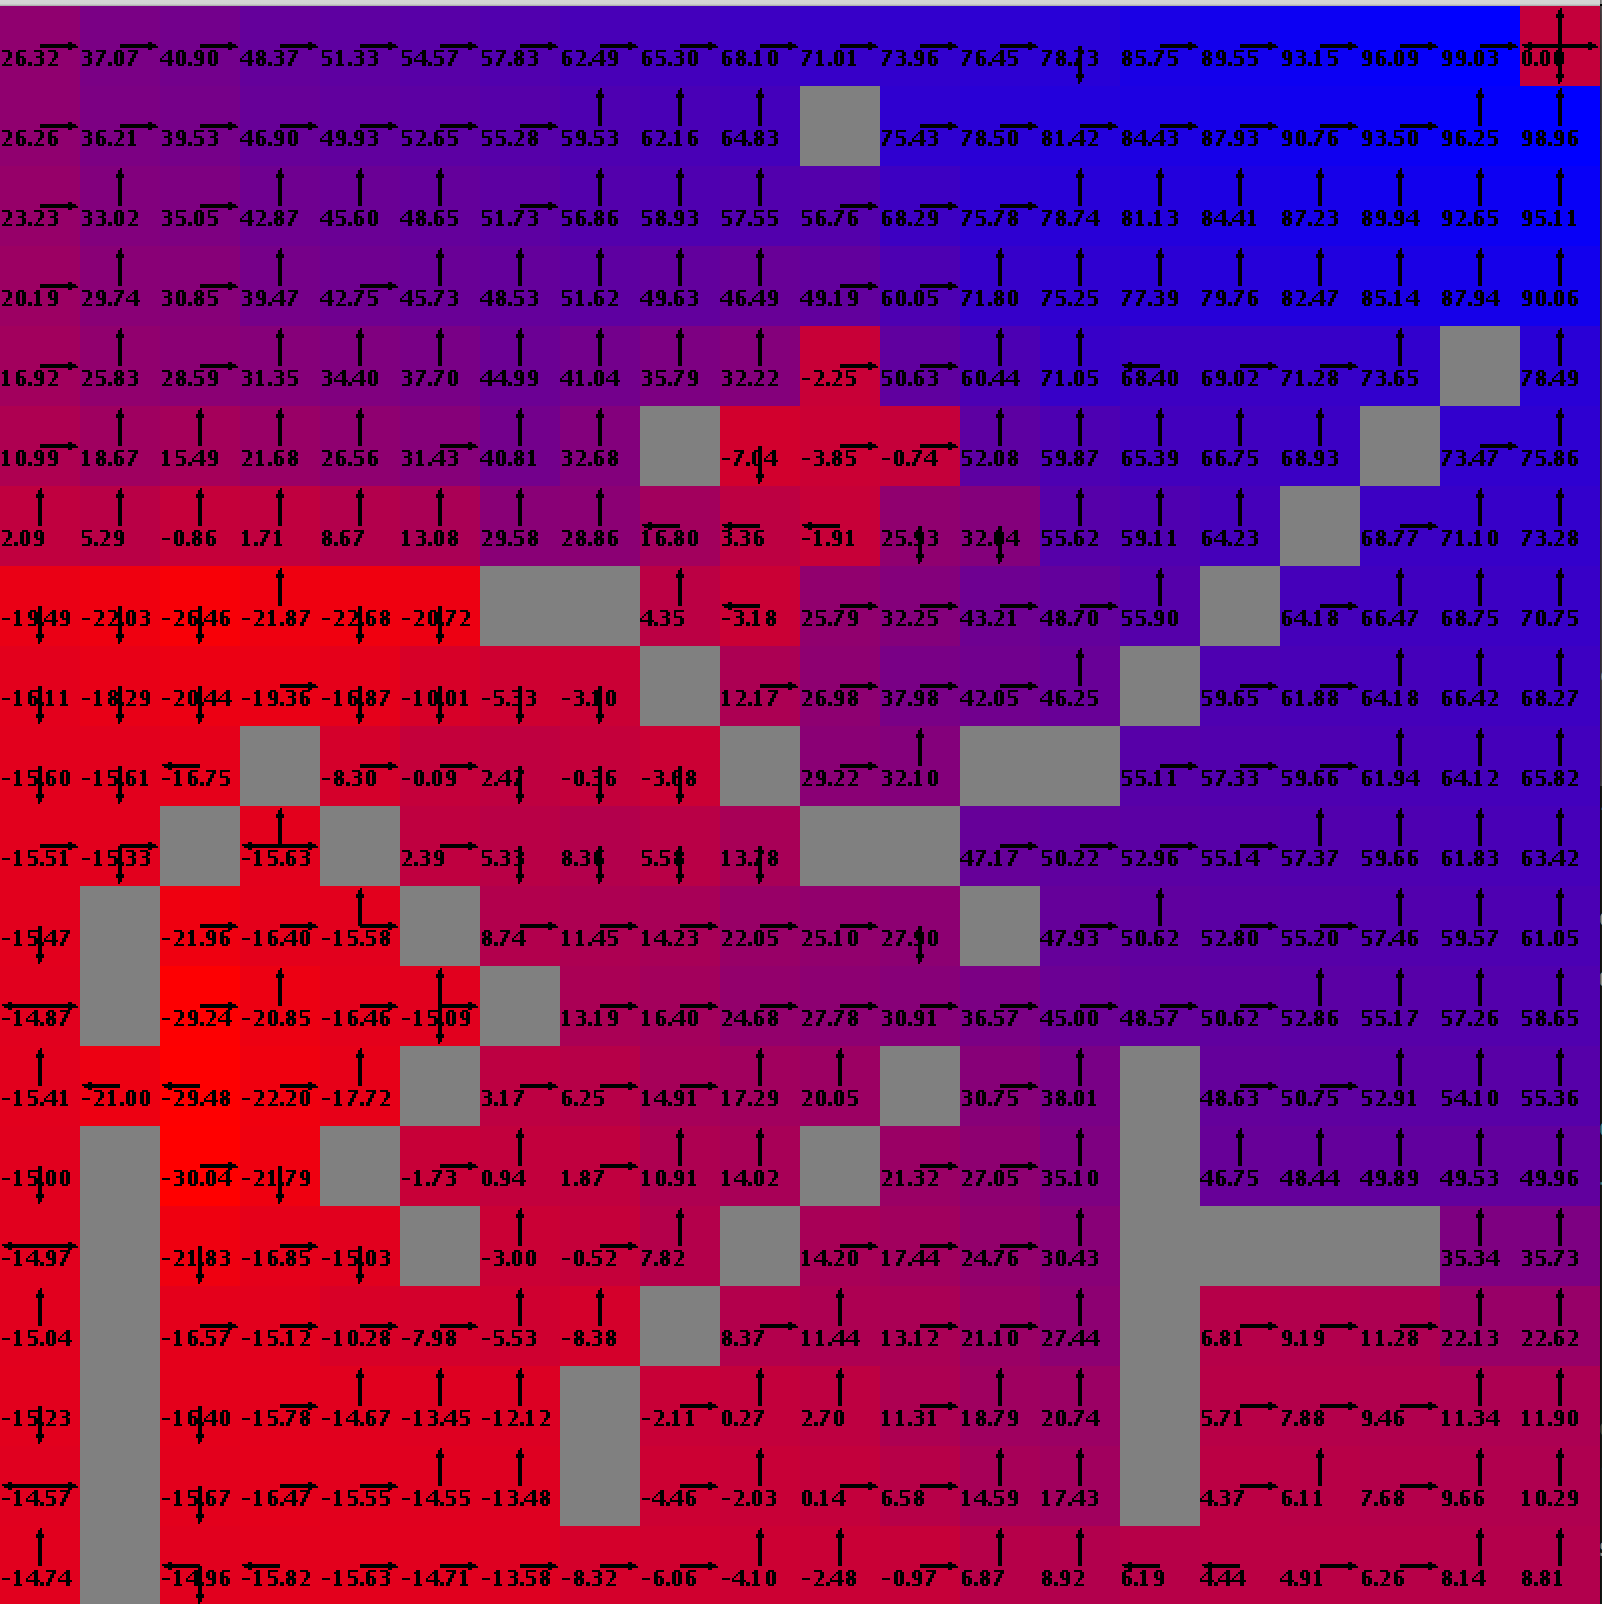
\includegraphics[width=1\textwidth,keepaspectratio]{hard-value-15.png} 
      \caption*{Hard GW Value Iteration \#15} 
   \endminipage\hfill
   \minipage{0.245\textwidth}
      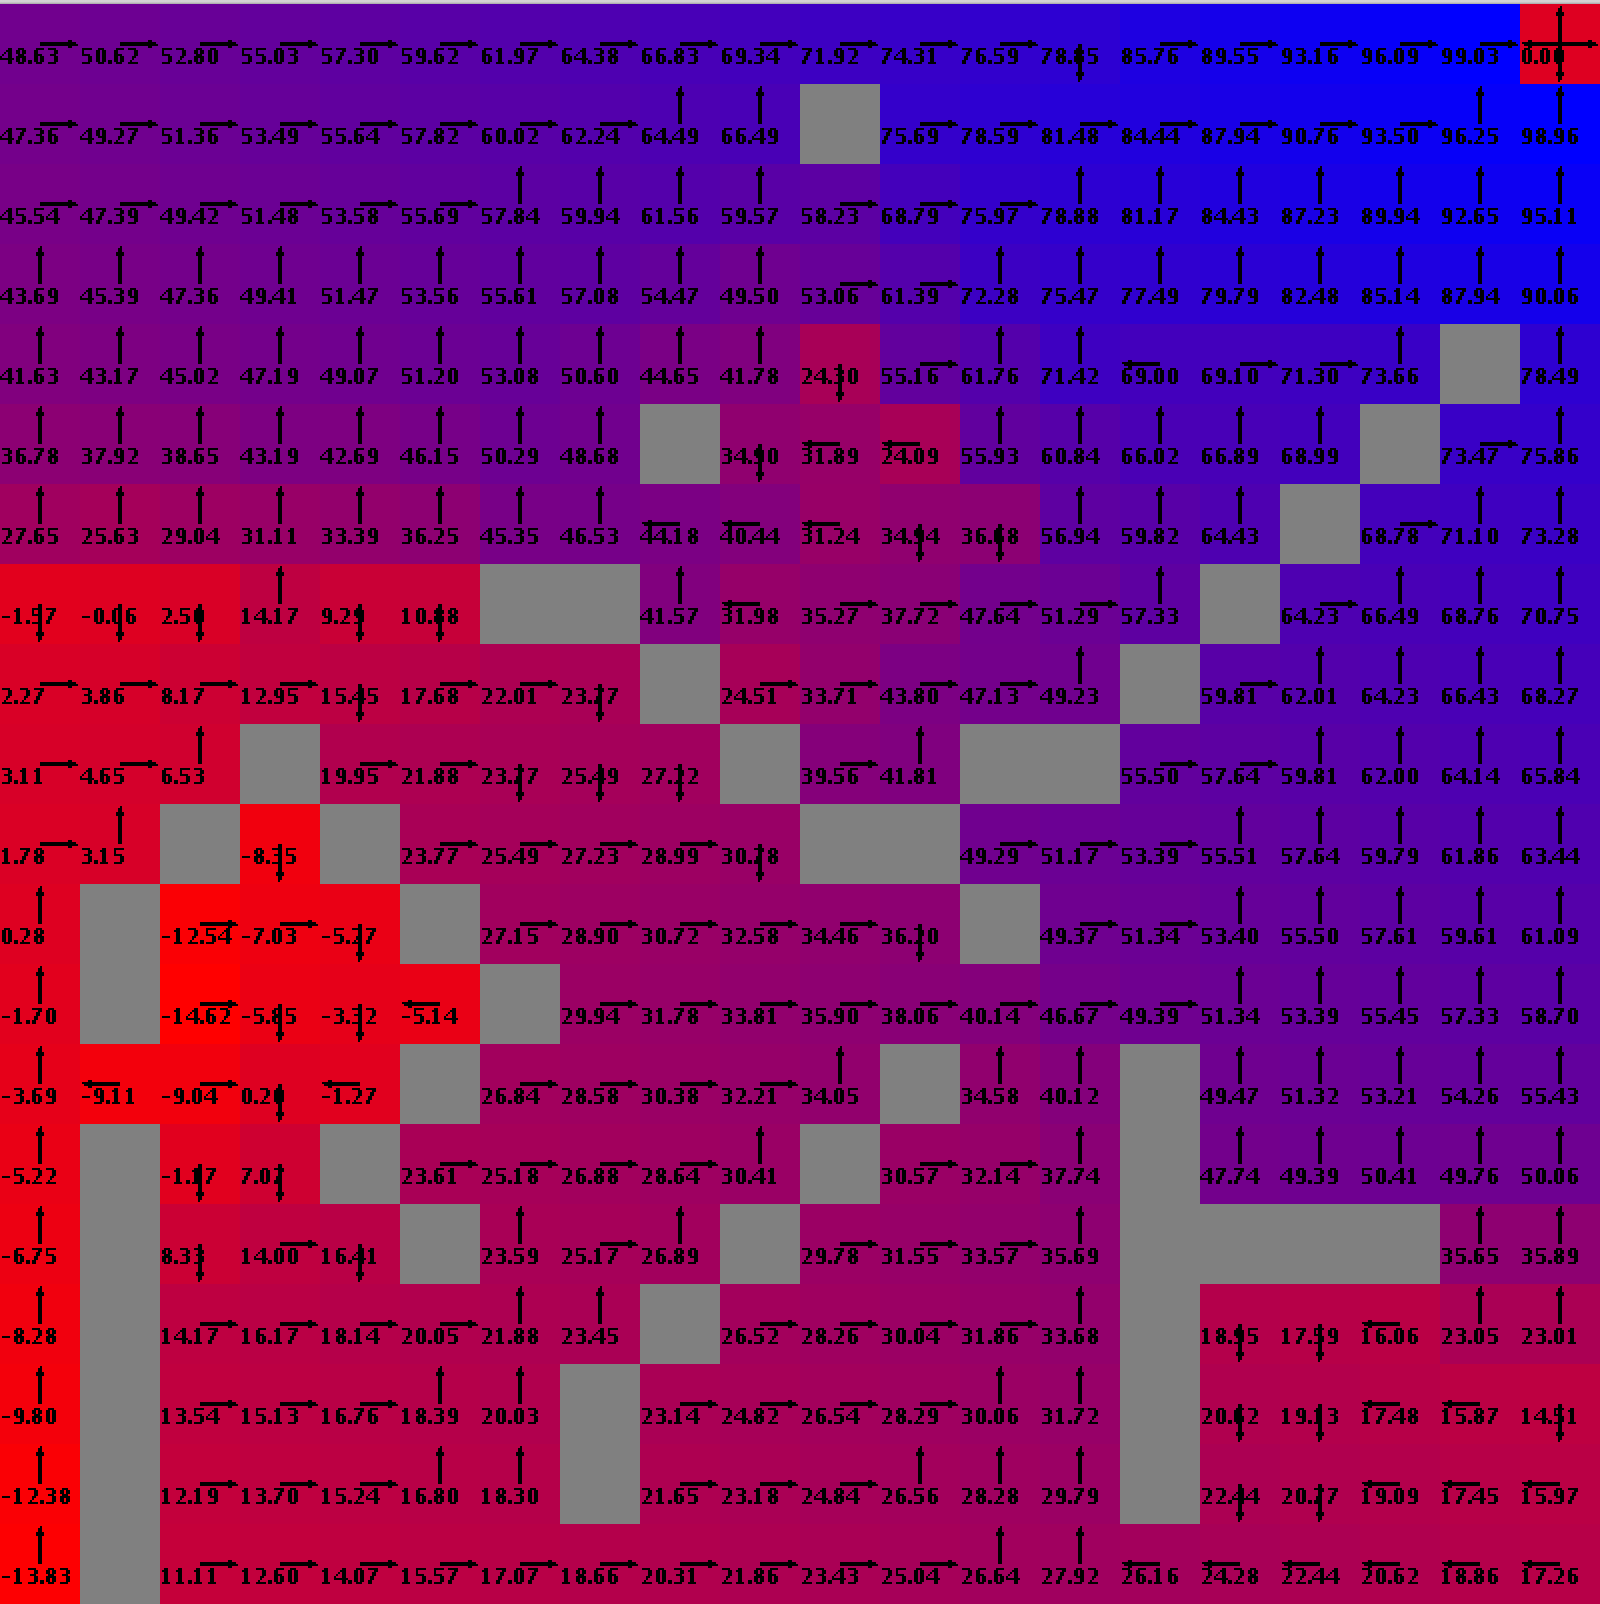
\includegraphics[width=1\textwidth,keepaspectratio]{hard-value-30.png} 
      \caption*{Hard GW Value Iteration \#30} 
   \endminipage\hfill
   \minipage{0.245\textwidth}
      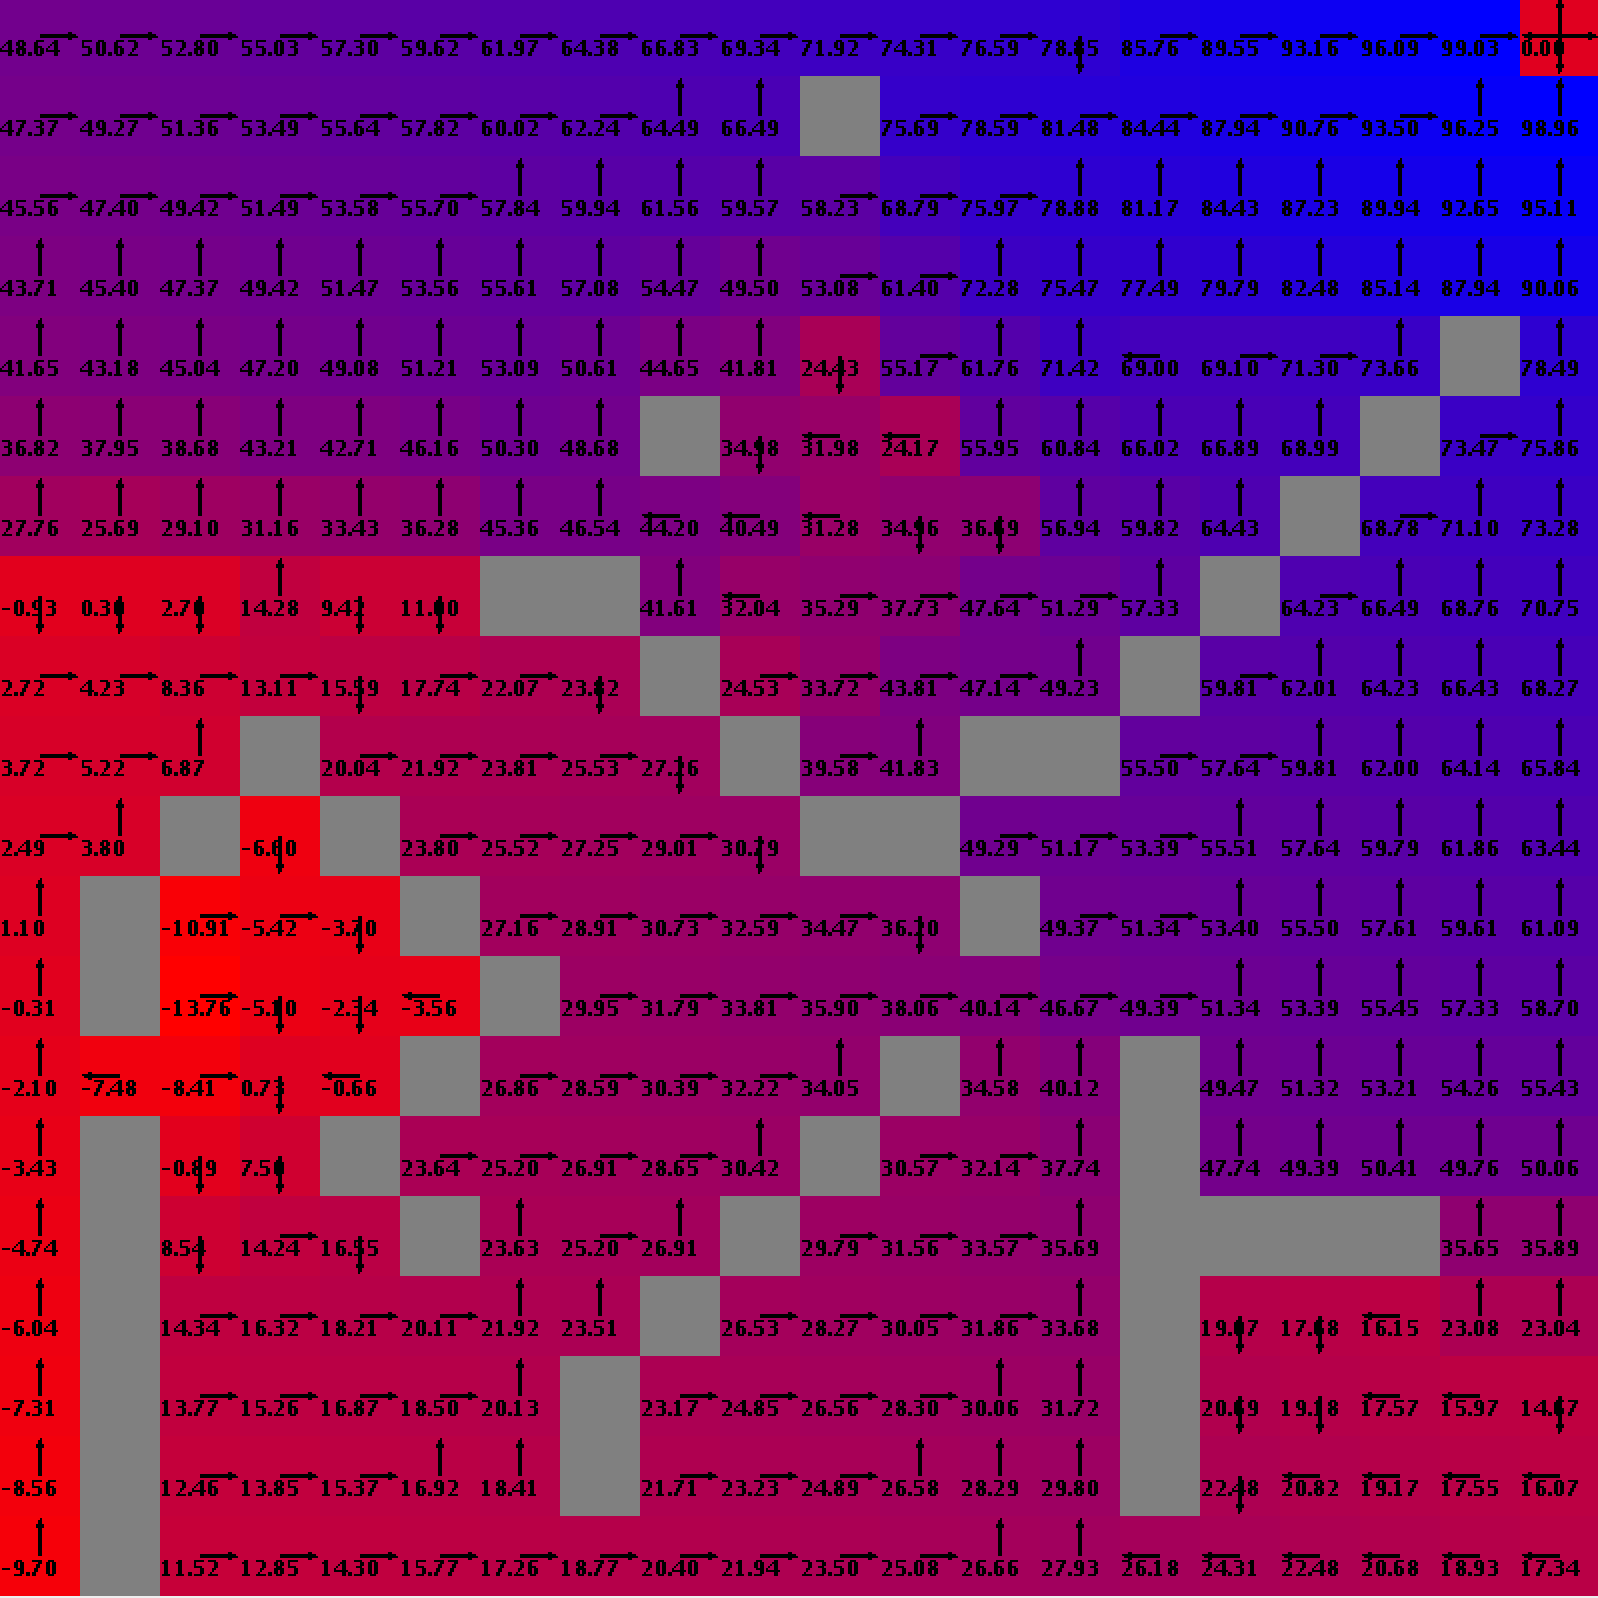
\includegraphics[width=1\textwidth,keepaspectratio]{hard-value-61.png} 
      \caption*{Hard GW Value Iteration \#61} 
   \endminipage\hfill
\end{figure}

 
\section*{Policy Iteration}
\subsection*{Introduction}
The second reinforcement learning algorithm used to optimally solve the MDPs is 
Policy Iteration.  Policy iteration works by beginning with a random policy and then 
attemping to modify it state by state by taking different actions.  This continues throughout each state of the policy in an attempt
 to find a better solution.  When no further policy changes are found, the algorithm 
 is finished.  Policy Iteration tends to take longer than Value Iteration due to 
 the additional number of explorations and calculations being done.
 
  \begin{figure}[H] 
\centering
\begin{tabular}{ | c | c  | c | c | c | c | c | c| c| c| c| c| c | } 
\hline
\textbf{Iterations} & \textbf{Time} & \textbf{Reward} & \textbf{Steps} & \textbf{Convergence}   \\
\hline
\textbf{EASY Gridworld} \\ \hline
1 & 0.0194 & -186.5000 & 190.9400 & 79.8000 \\ \hline
5 & 0.1096 & 43.1000 & 25.2600 & 22.2546 \\ \hline
10 & 0.2077 & 45.2200 & 49.3200 & 3.0887 \\ \hline
15 & 0.2406 & 44.0200 & 48.4200 & 0.0007 \\ \hline
20 & 0.2568 & 44.8400 & 50.6800 & 0.0002 \\ \hline
25 & 0.2747 & 46.0200 & 45.9800 & 1.58e-5 \\ \hline
30 & 0.2907 & 46.7800 & 48.4800 & 2.19e-6 \\ \hline
33 & 0.3021 & 47.9400 & 45.5800 & 8.23e-7 \\ \hline
\\
\textbf{HARD Gridworld} \\ \hline
1 & 0.3033 & -299 & 300 & 83.8936 \\ \hline
5 & 0.9030 & -258.4100 & 267.2600 & 60.8785 \\ \hline
10 & 1.6424 & 10.9300 & 63.3000 & 39.2628 \\ \hline
15 & 2.2504 & 11.5600 & 63.1000 & 1.5369 \\ \hline
20 & 2.4257 & 10.3800 & 64.2100 & 5.11e-6 \\ \hline
22 & 2.4633 & 9.9600 & 64.2300 & 8.07e-7 \\ \hline

\end{tabular}
\caption*{Gridworld Policy Iteration Results} 
\end{figure}


 \subsubsection*{Easy Gridworld Policy Iteration Results}
Here we examine policy iteration for the easy gridworld pathfinding experiment.  To measure converge, an iteration threshold of 1e-6 is used.  For this 
 gridworld problem, it takes 33 iterations for policy iteration's policy delta to converge 
 below the threshold.  While the policy iteration approach starts to converge 
 very quickly, it starts to level off and does not see substantial benefits 
 after approximately 10 iterations--which can also be observed in the policy map 
 graphics below.
 \\ \\
 In terms of performance, the maximum reward value is found at iteration \#33--indicating 
 that that policy iteration found an optimal policy as it converged.  At 48 steps, the journey 
 taken is much more complex than the naive solutions found at early iterations but optimized further than similarly high reward policies.  
  In terms of iteration time, the algorithm is rather fast--which is aided by the fact that only 33 steps are needed for convergence.
   Looking at the policy maps, it is evident that policy iteration performs very well for this problem. 
 
  \subsubsection*{Hard Gridworld Policy Iteration Results}
 Using a similar converence approach to above, converge is acheived even 
 earlier--at only 22 iterations.  The biggest change is between iterations 10 and 15 
 iterations, after which things somewhat level off before hitting \#22.  In this 
 case, the policy iteration approach fairs very well since it is able to branch 
 off and positively manipulate as it progress from state to state.  The policy 
 maps included below do a great job of displaying so.
 \\ \\
 Performance-wise, the maximum reward is found at one of the middle iterations--\#15.  At 63 steps and higher rewards, the path is much more optimal than initial trials.
  It takes nearly 2 and half seconds to converge--which is markedly longer for 
  the hard grid than the easy grid.  Still, at the end of the day, policy 
  iteration does a fantastic job at determining an optimal policy.
 
 
    \begin{figure}[H]
  \minipage{0.245\textwidth}
      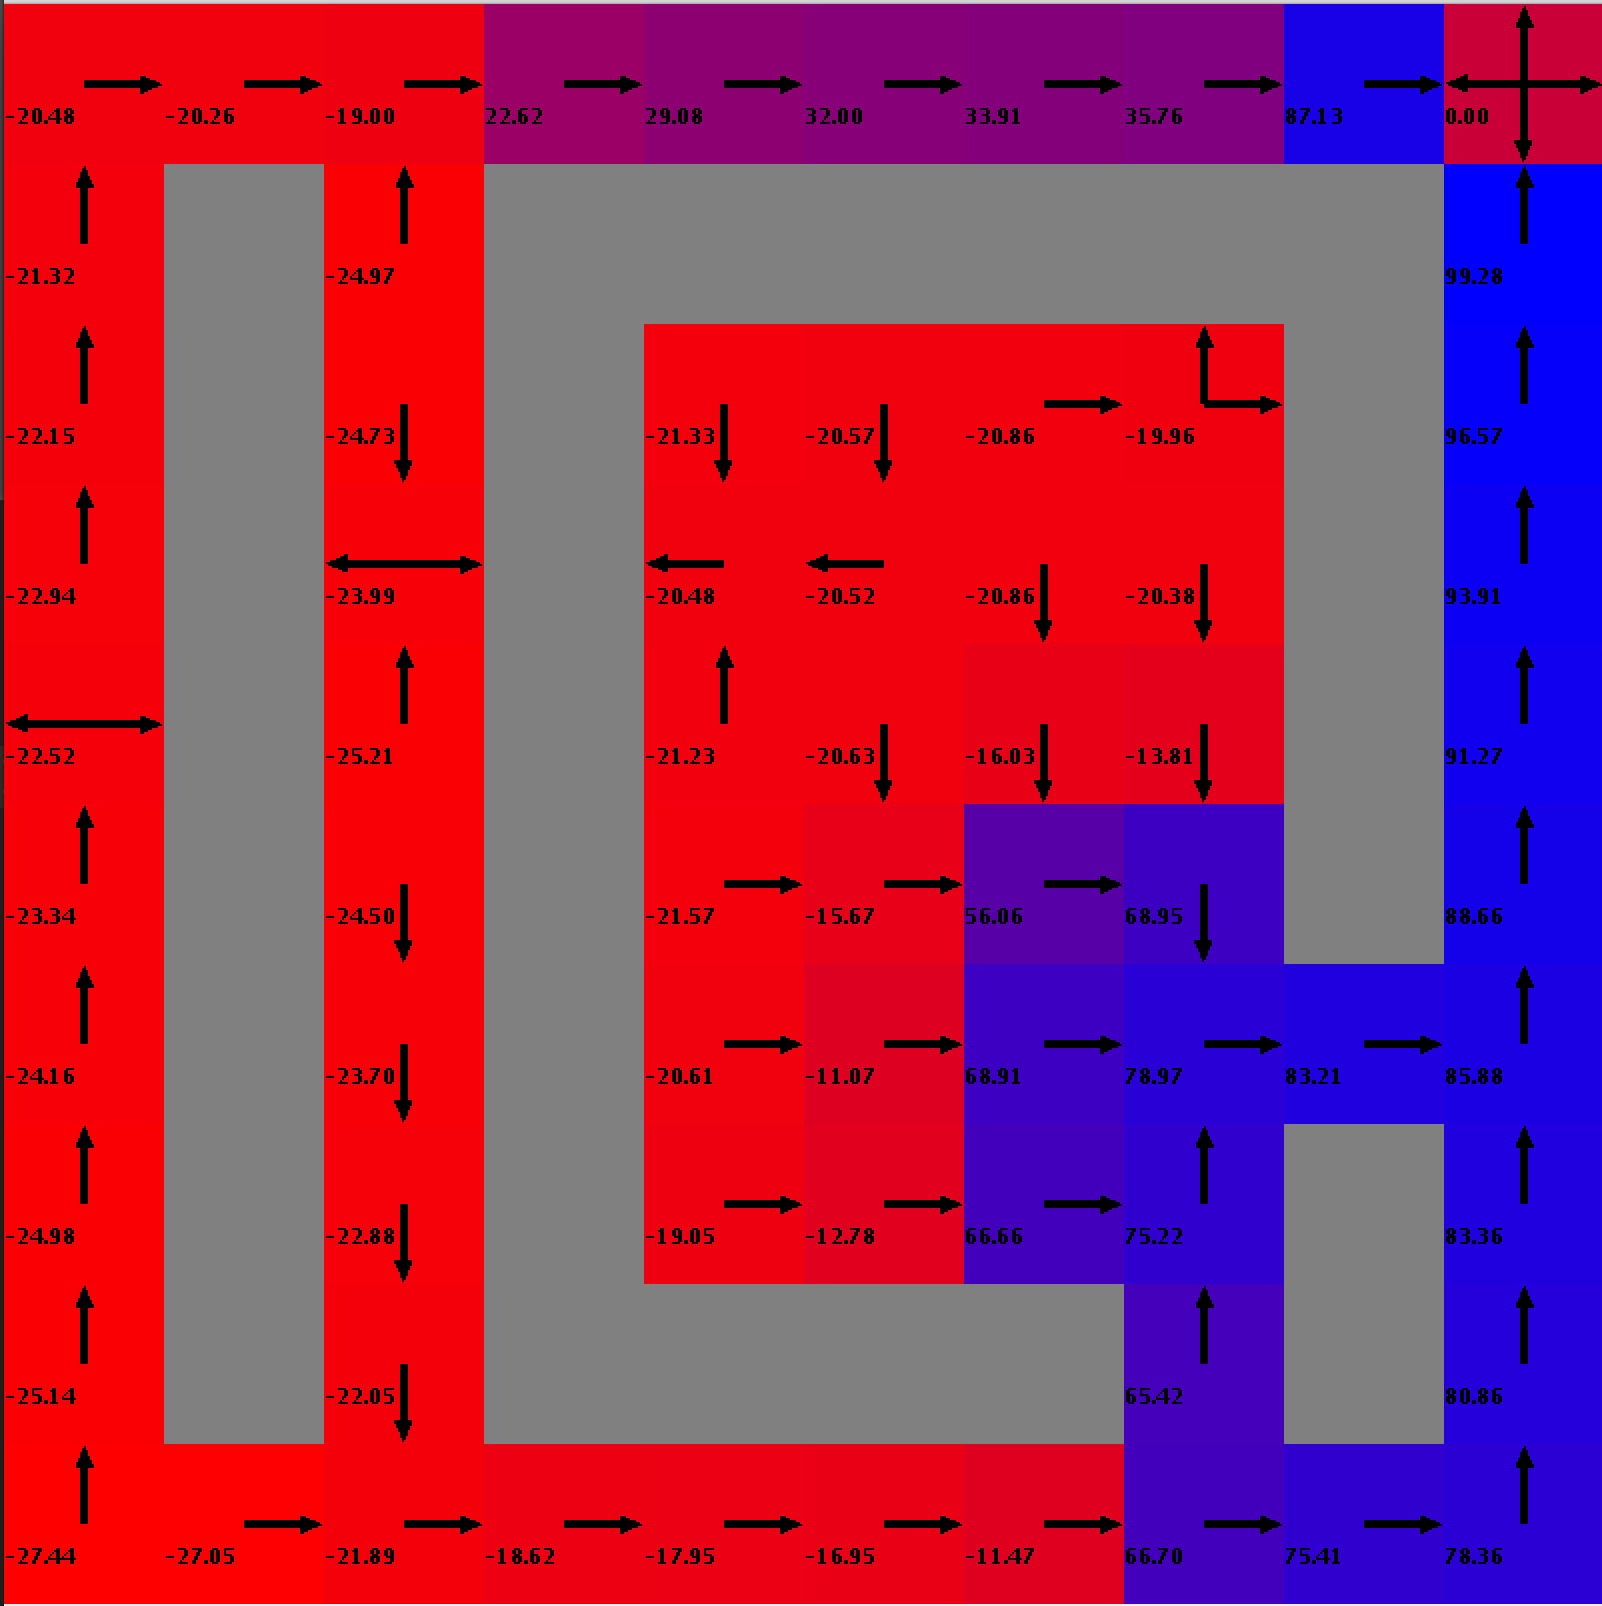
\includegraphics[width=1\textwidth,keepaspectratio]{easy-policy-2.png} 
      \caption*{Easy GW Policy Iteration \#2} 
   \endminipage\hfill
   \minipage{0.245\textwidth}
      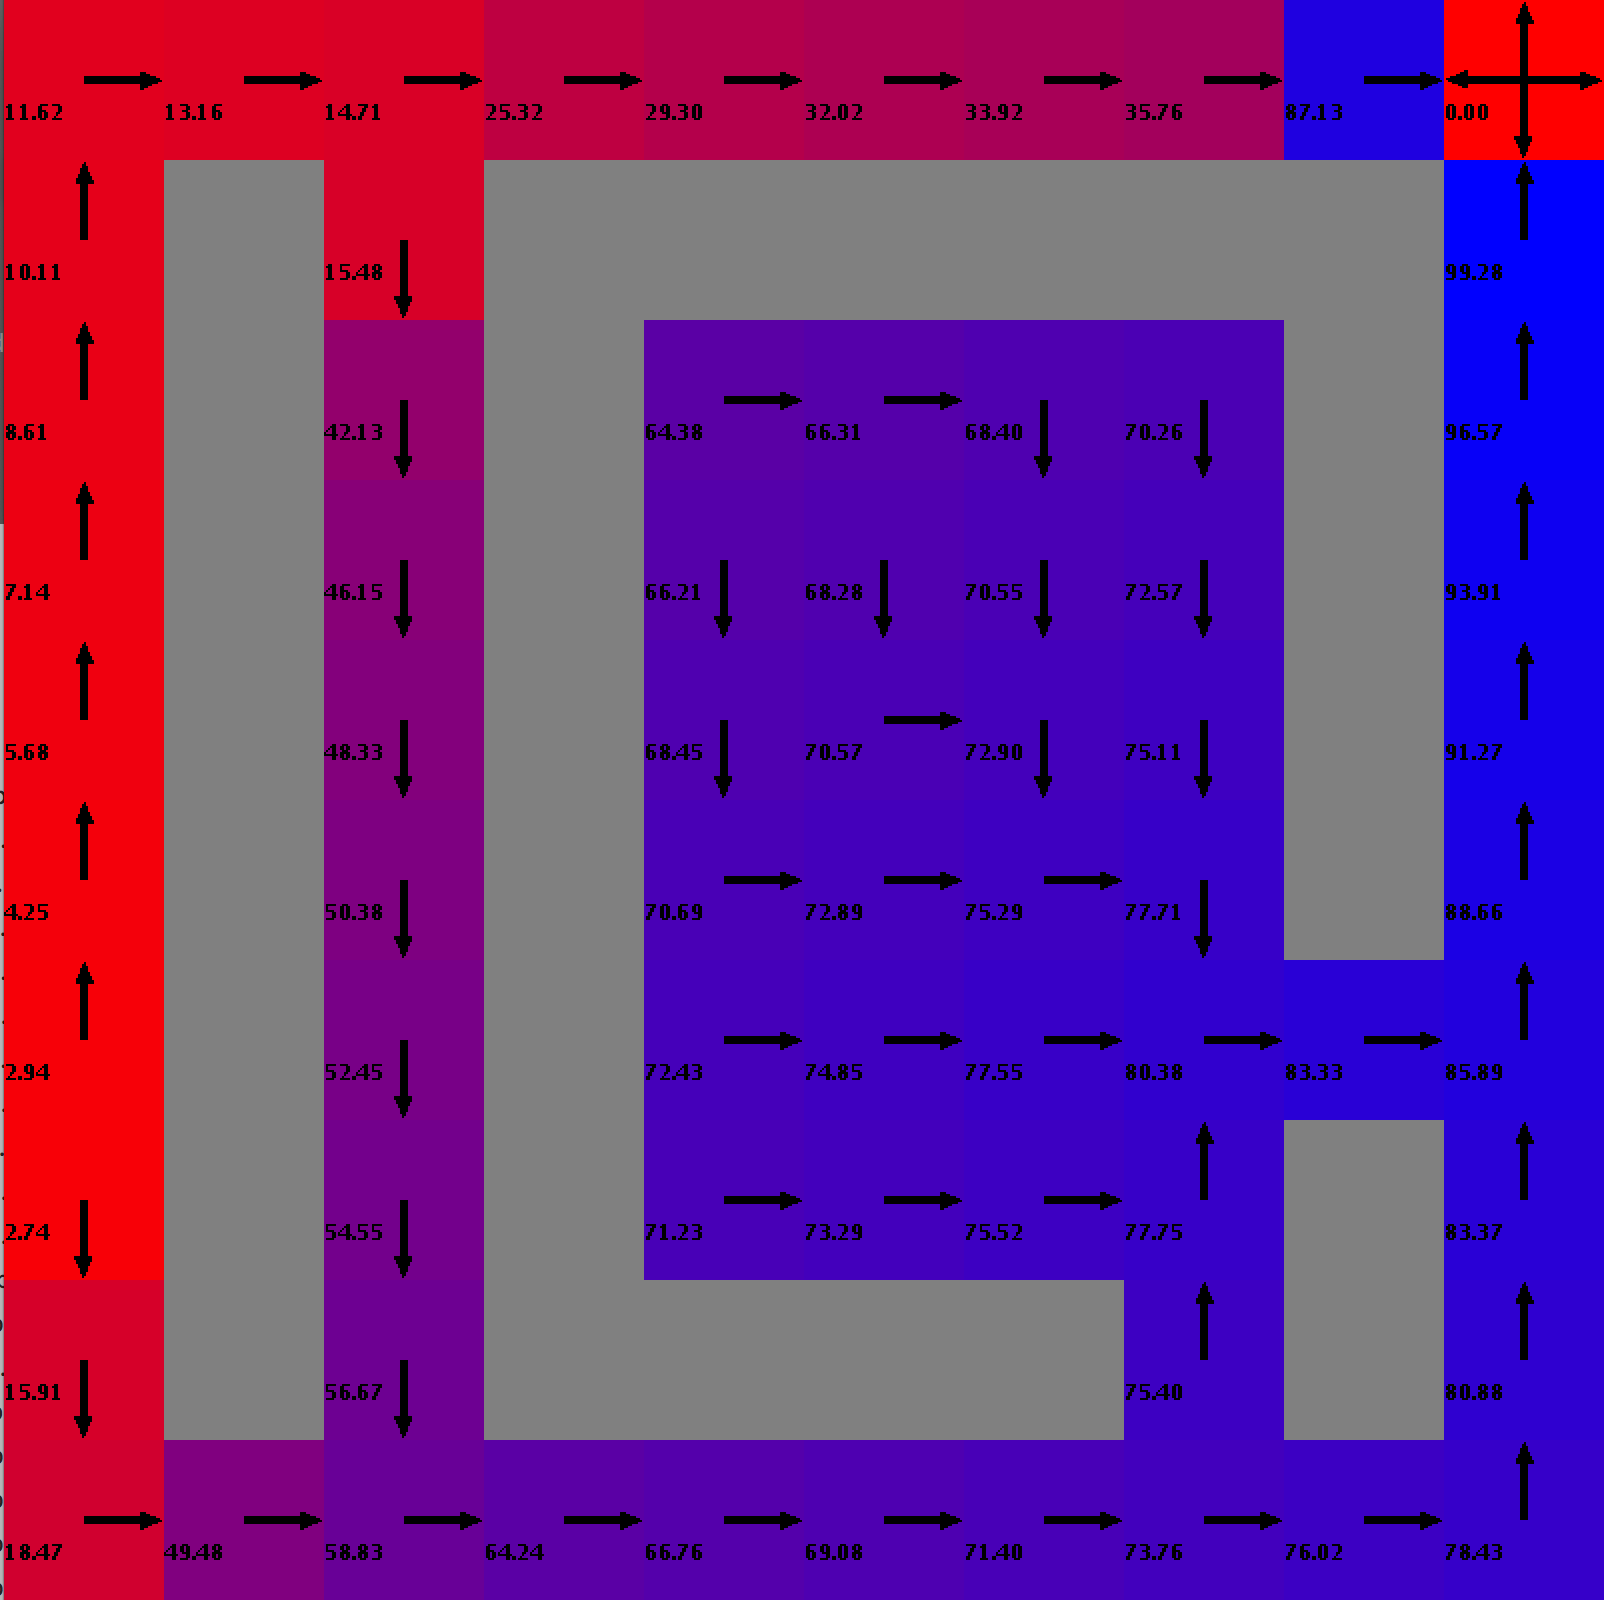
\includegraphics[width=1\textwidth,keepaspectratio]{easy-policy-5.png} 
      \caption*{Easy GW Policy Iteration \#5} 
   \endminipage\hfill
   \minipage{0.245\textwidth}
      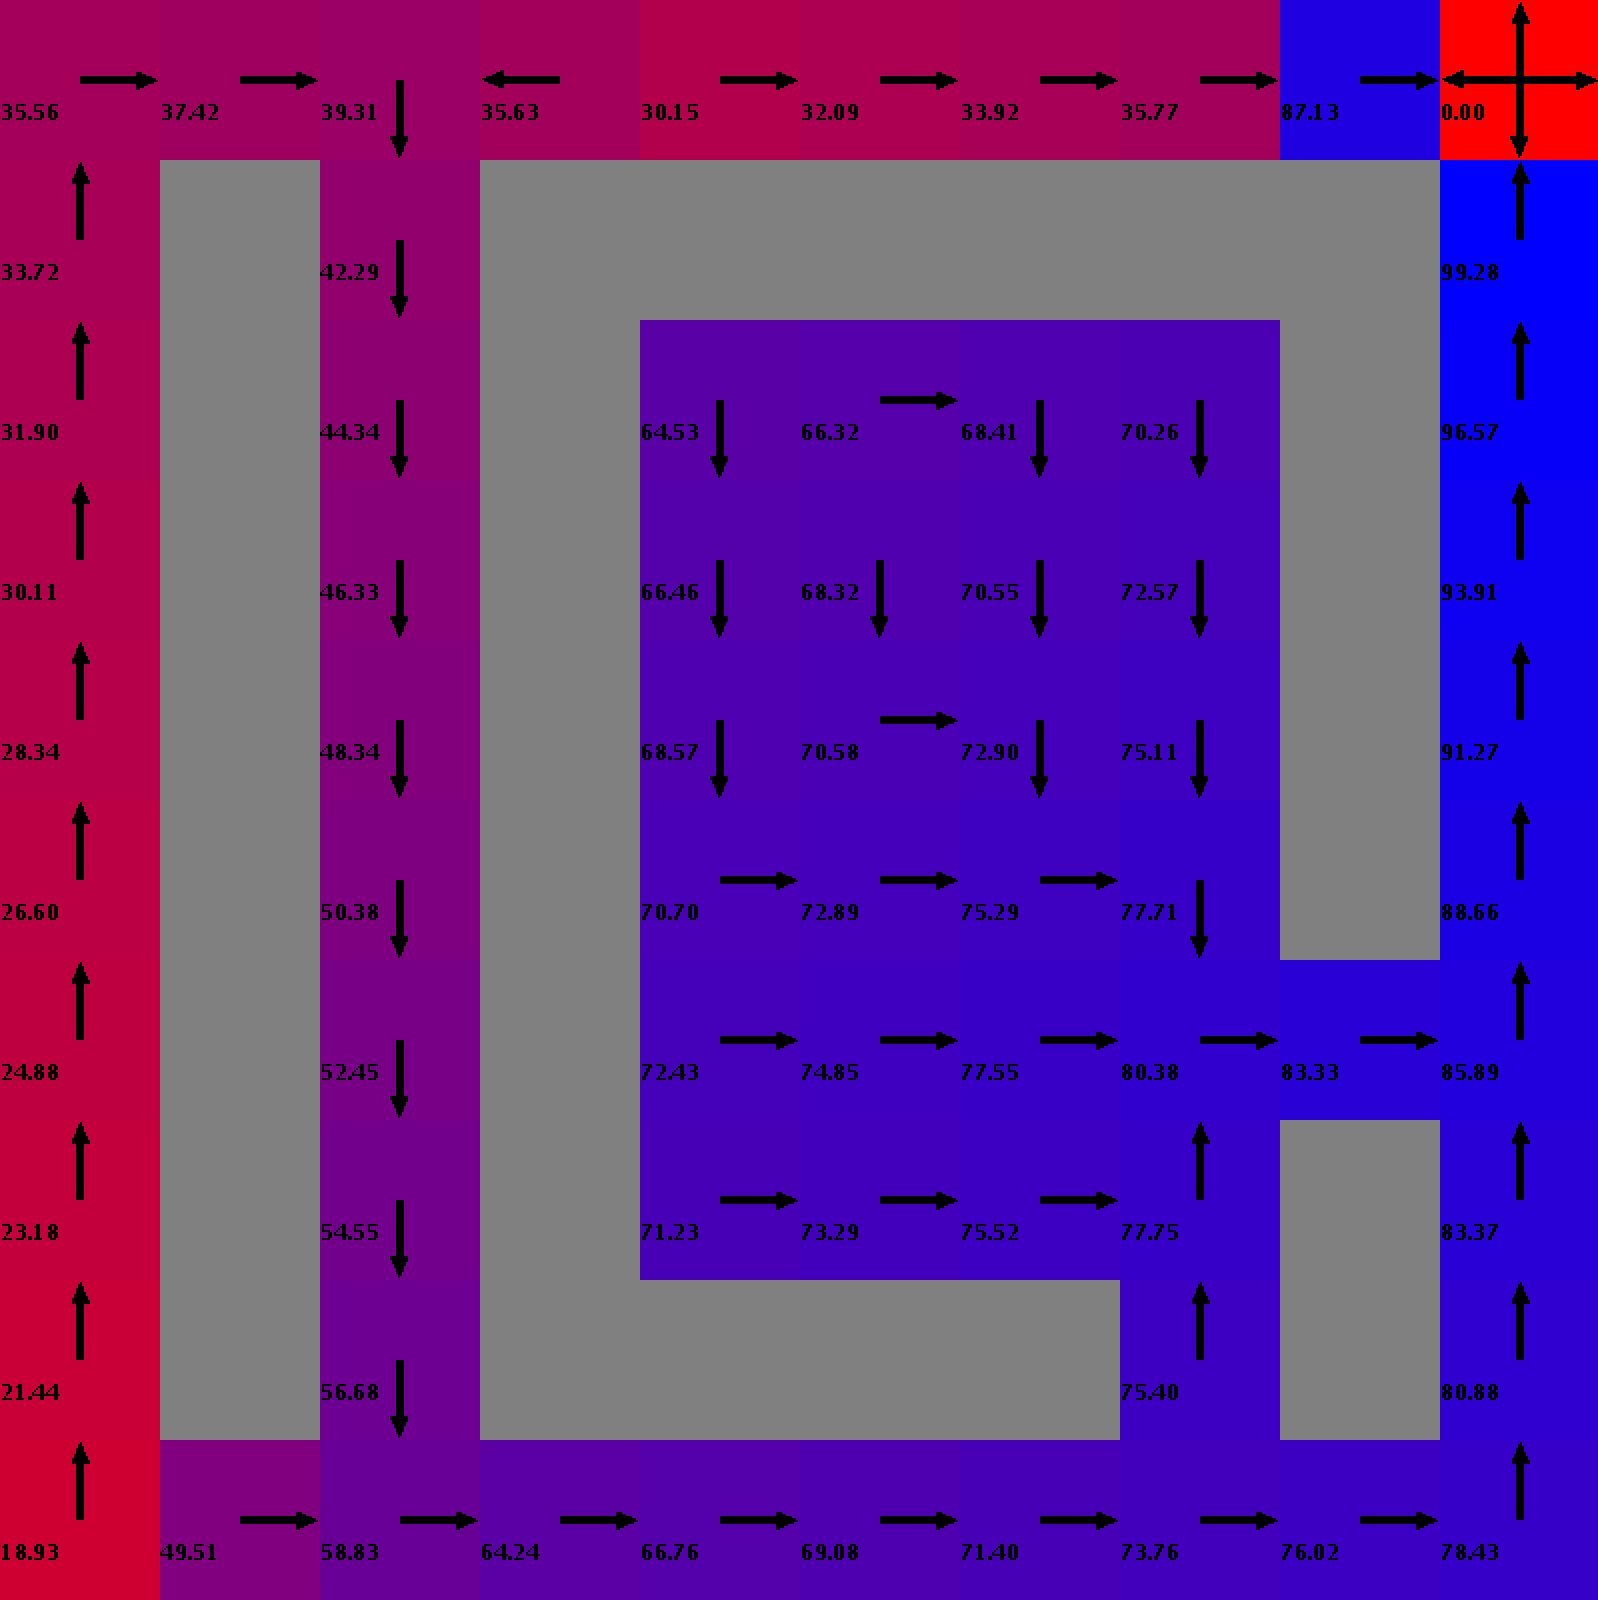
\includegraphics[width=1\textwidth,keepaspectratio]{easy-policy-10.png} 
      \caption*{Easy GW Policy Iteration \#10} 
   \endminipage\hfill
   \minipage{0.245\textwidth}
      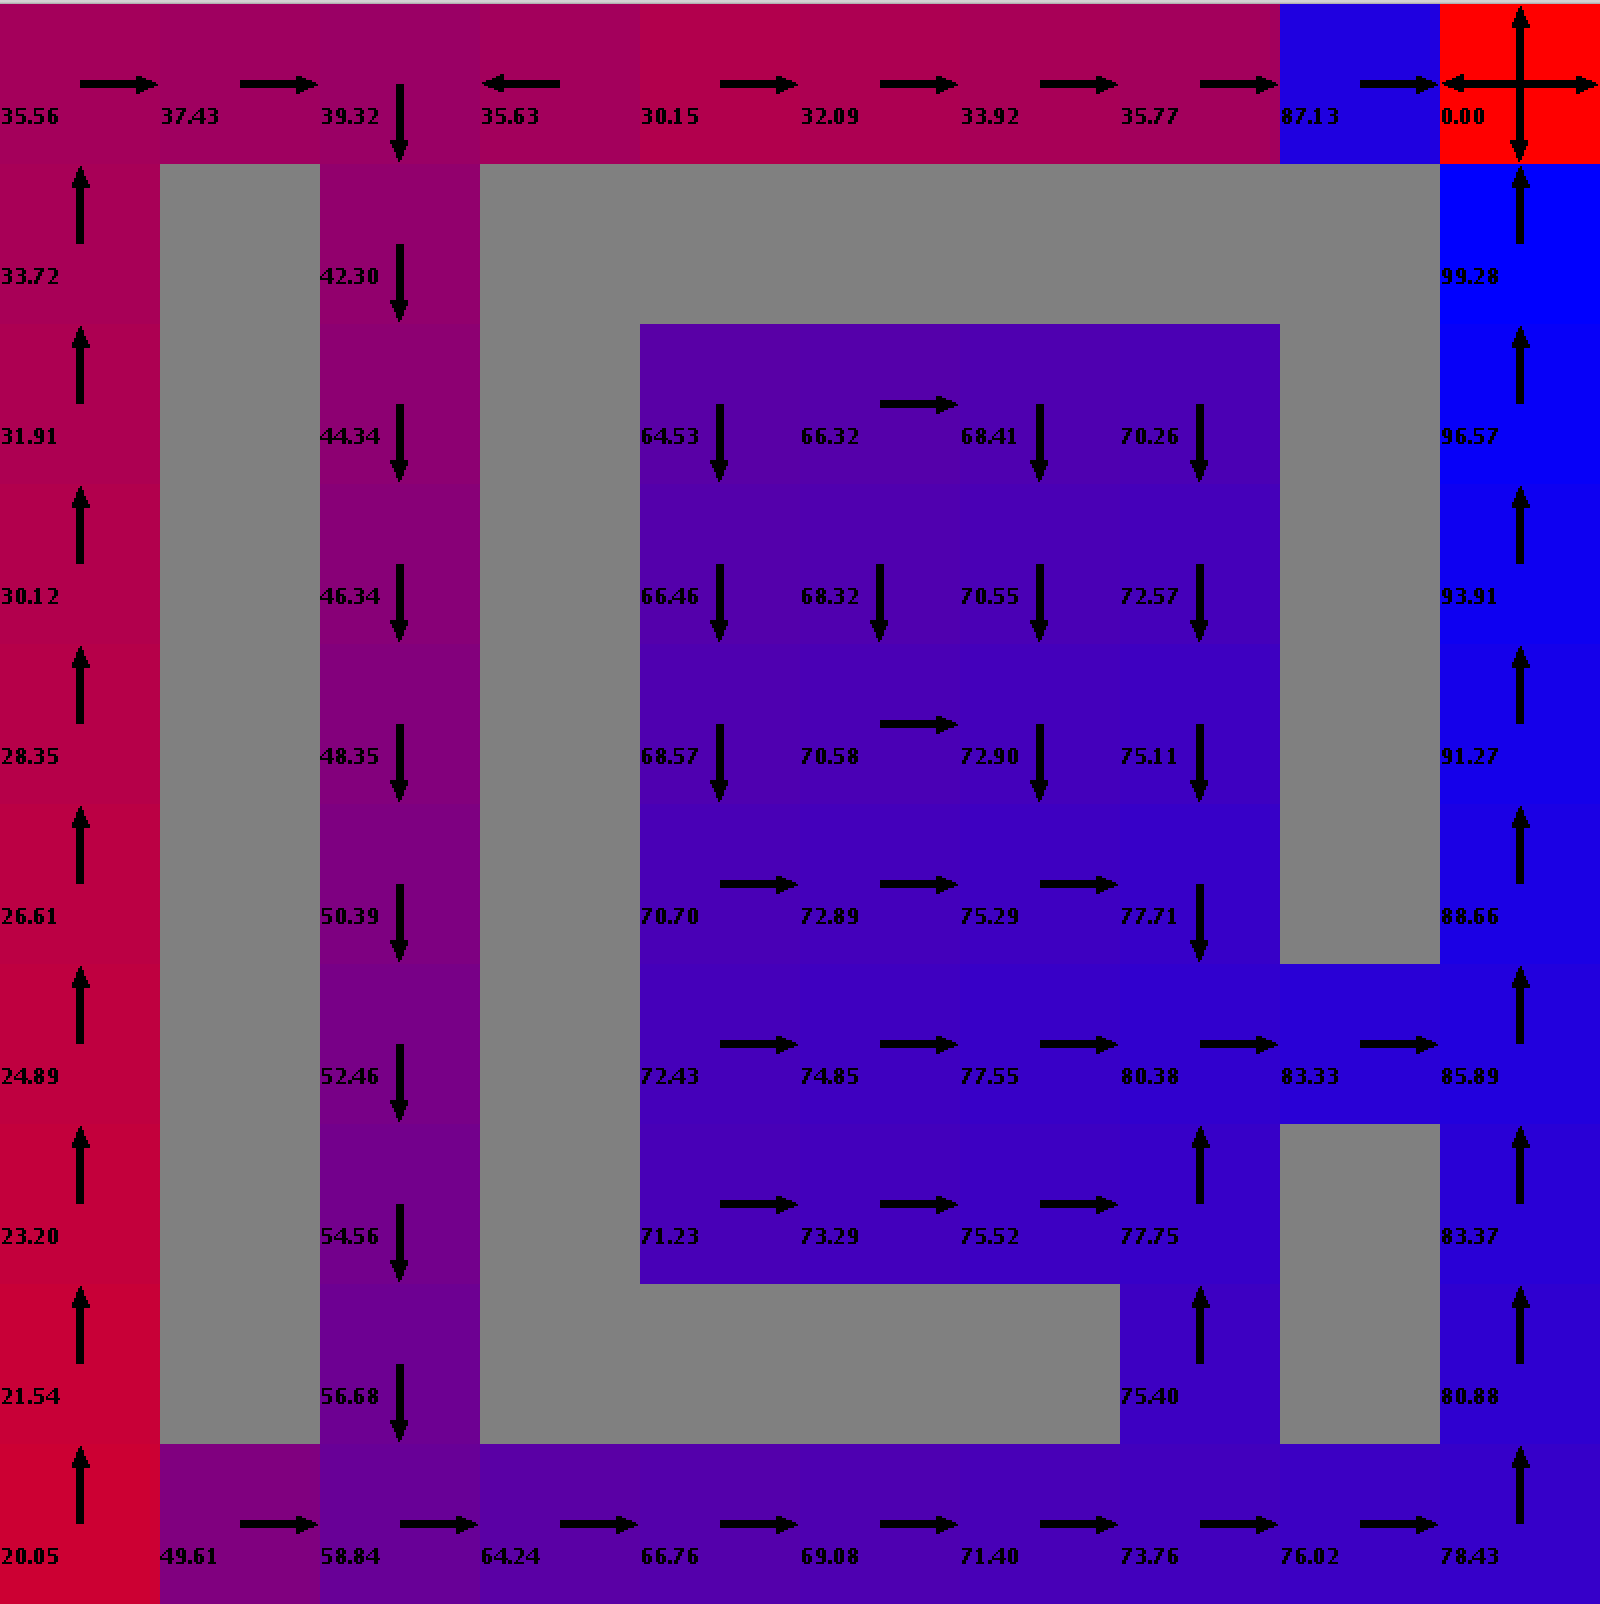
\includegraphics[width=1\textwidth,keepaspectratio]{easy-policy-33.png} 
      \caption*{Easy GW Policy Iteration \#33} 
   \endminipage\hfill
\end{figure}


   \begin{figure}[H]
  \minipage{0.245\textwidth}
      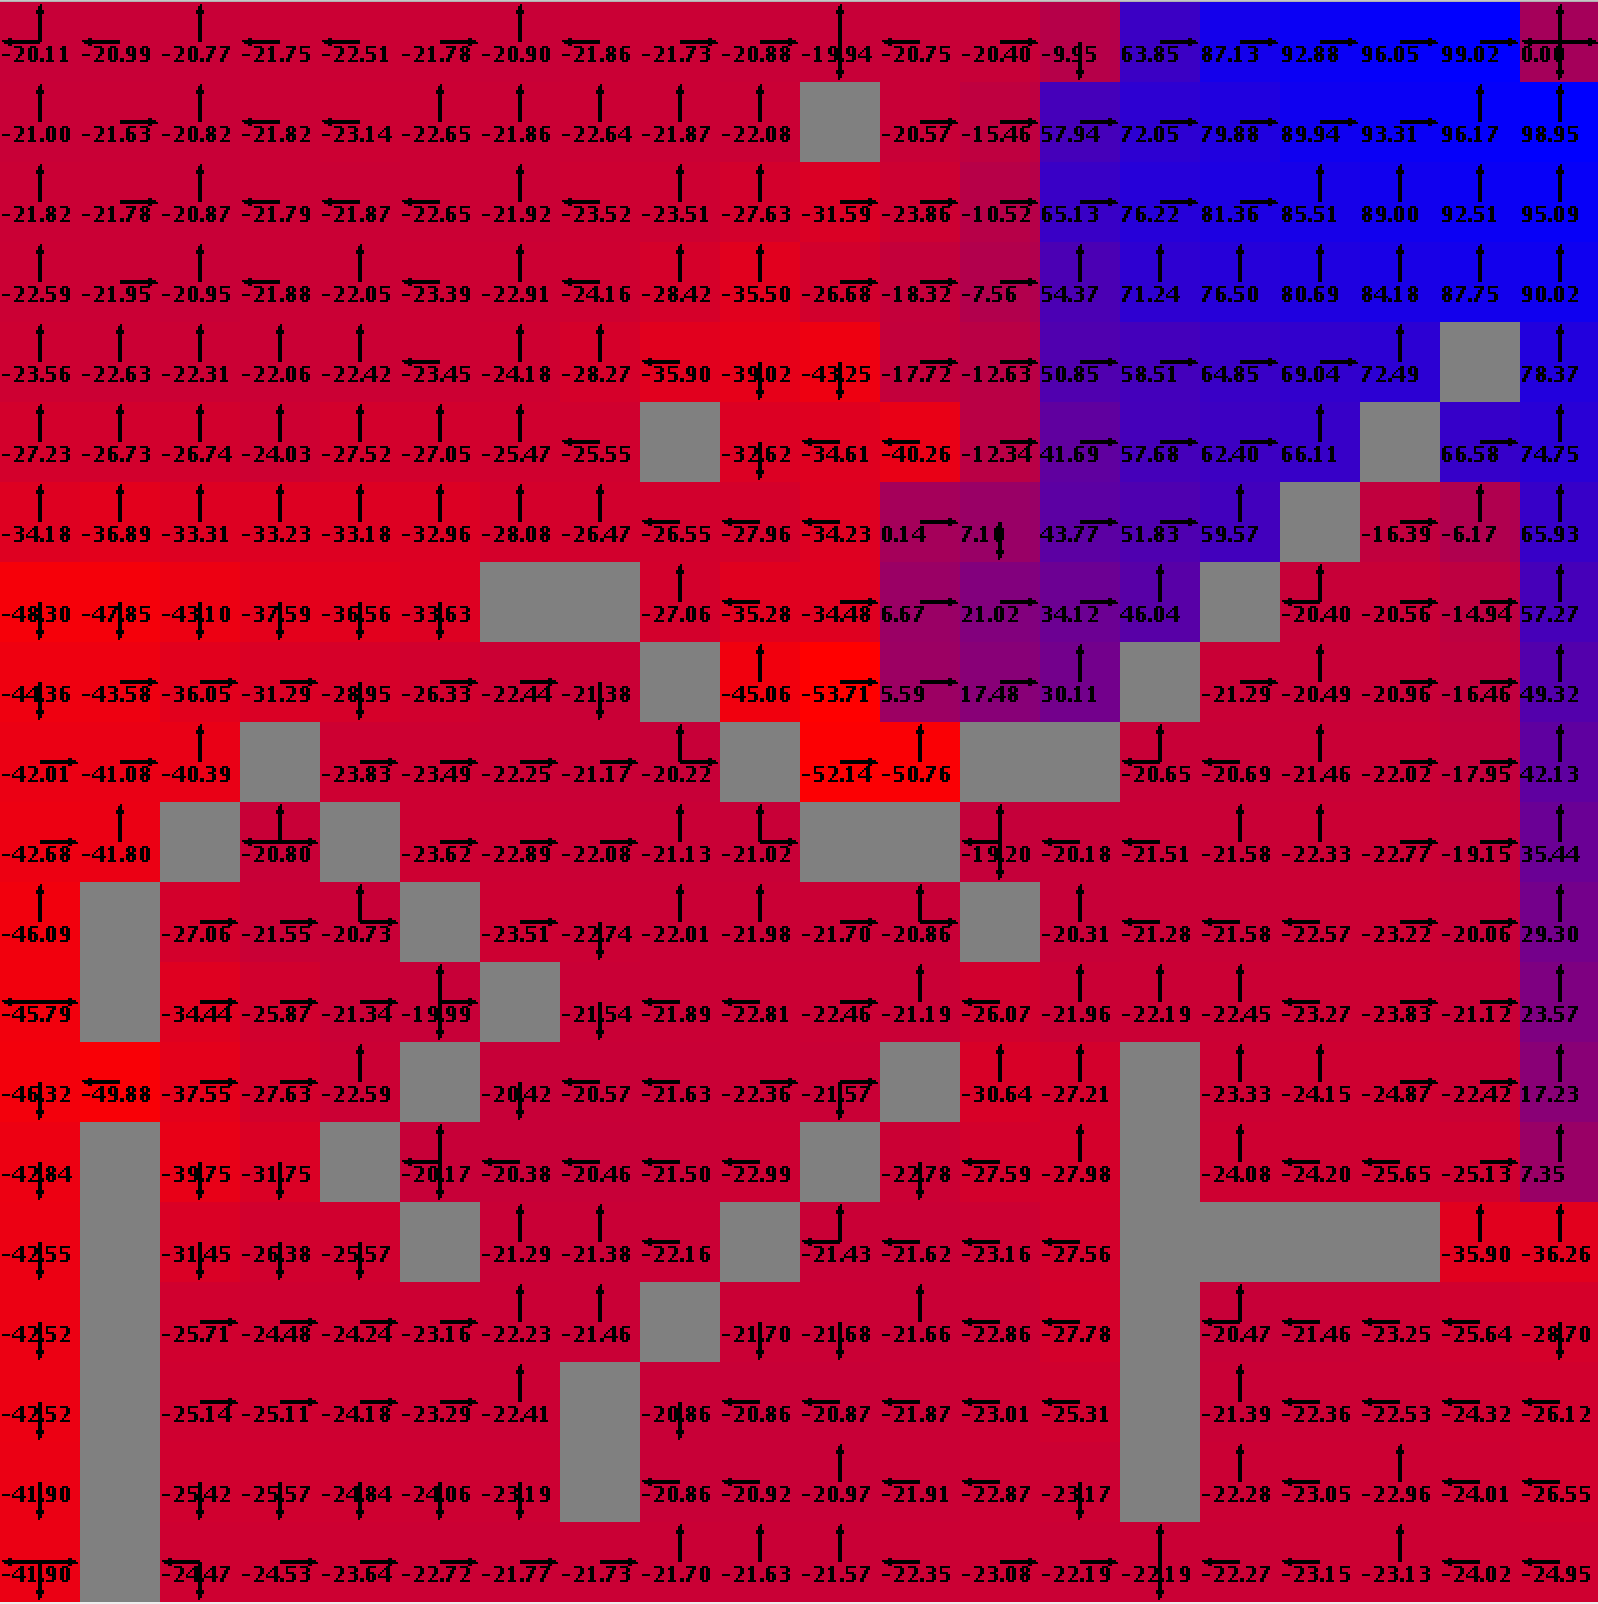
\includegraphics[width=1\textwidth,keepaspectratio]{hard-policy-2.png} 
      \caption*{Hard GW Policy Iteration \#2} 
   \endminipage\hfill
   \minipage{0.245\textwidth}
      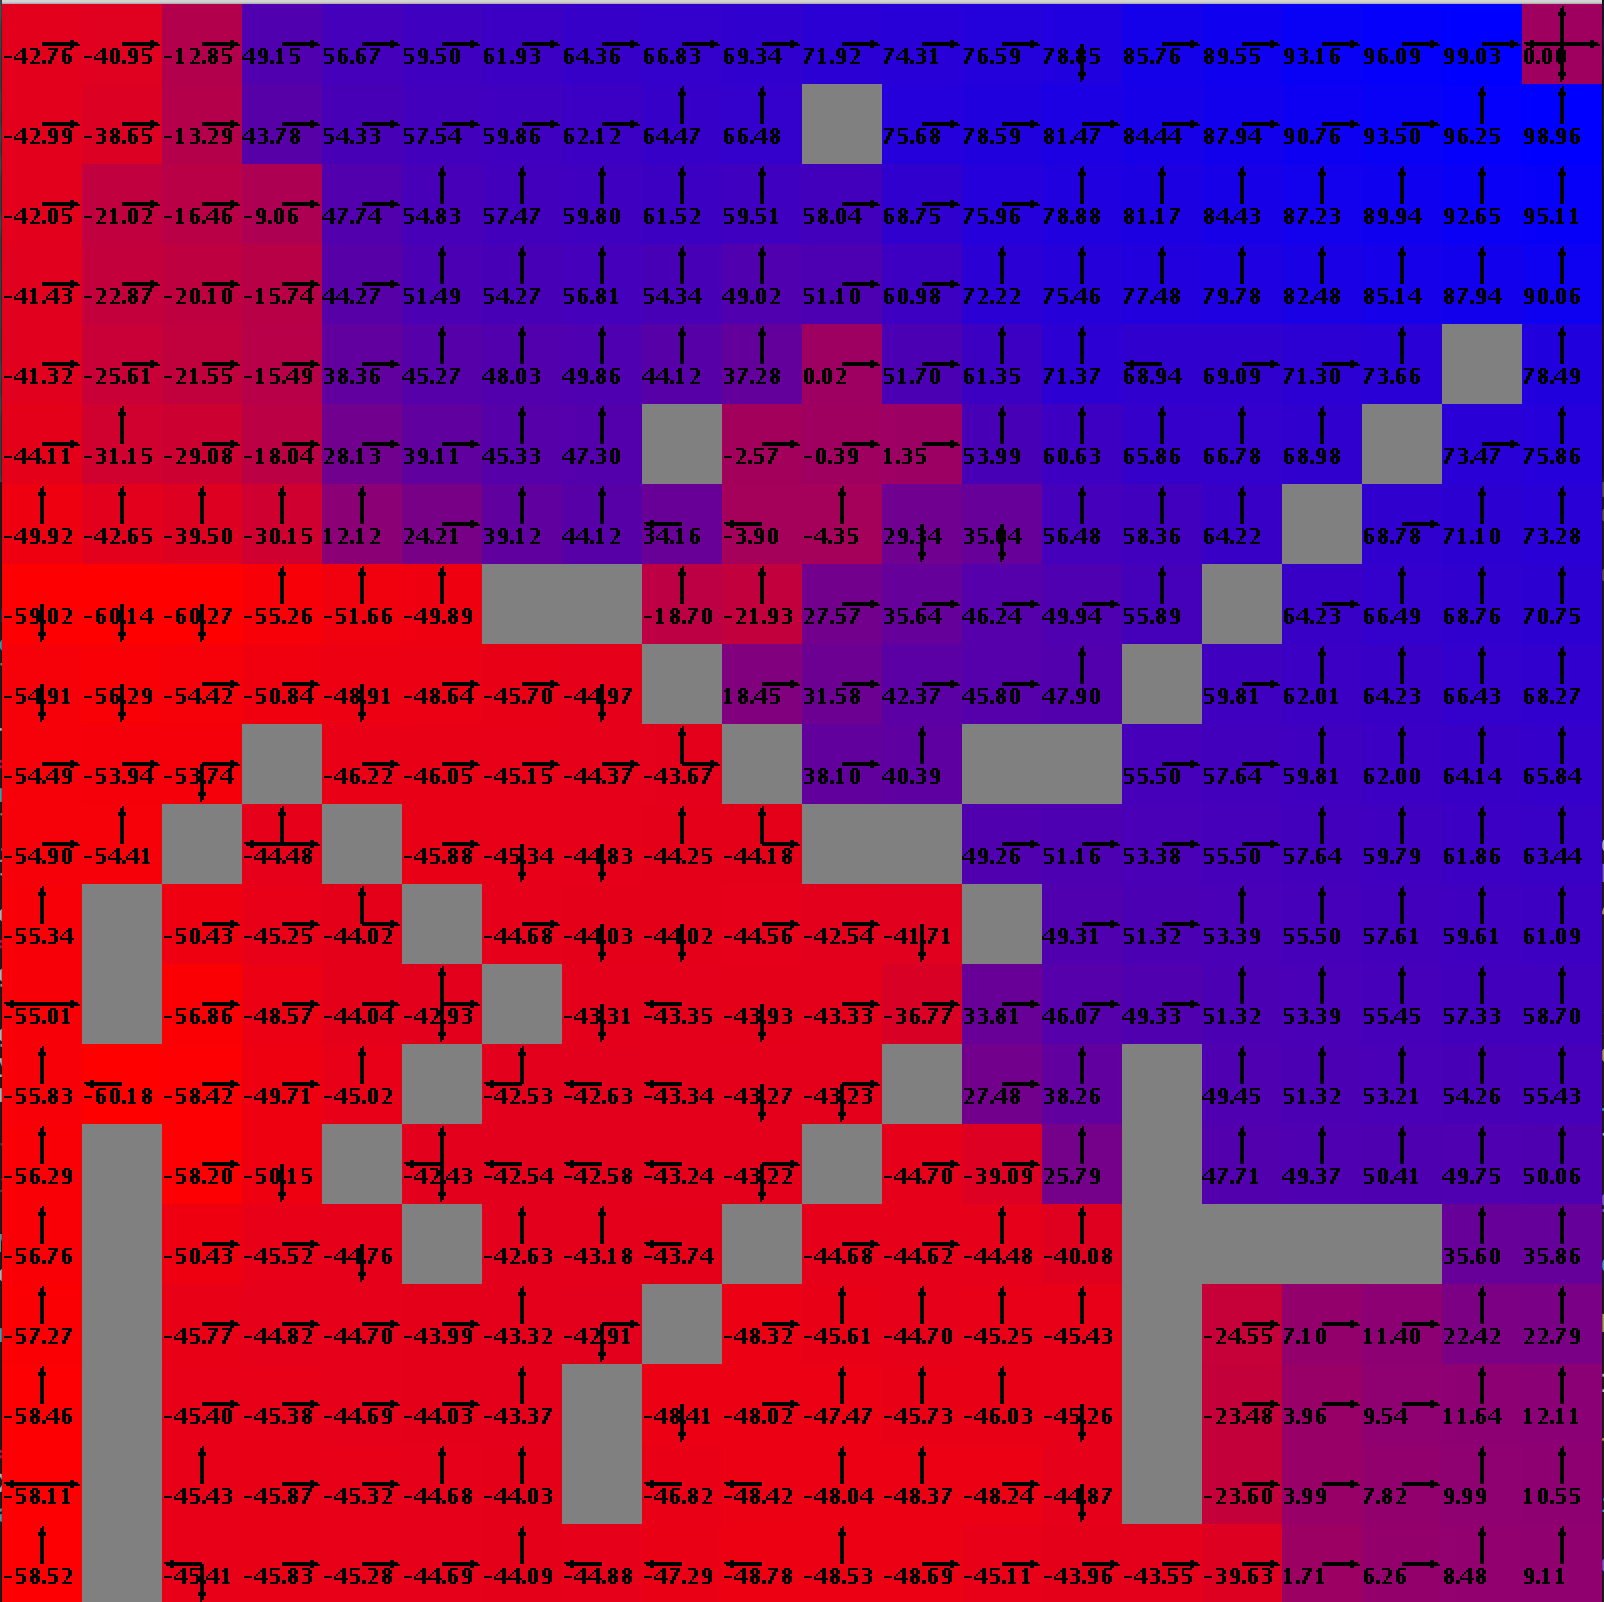
\includegraphics[width=1\textwidth,keepaspectratio]{hard-policy-5.png} 
      \caption*{Hard GW Policy Iteration \#5} 
   \endminipage\hfill
   \minipage{0.245\textwidth}
      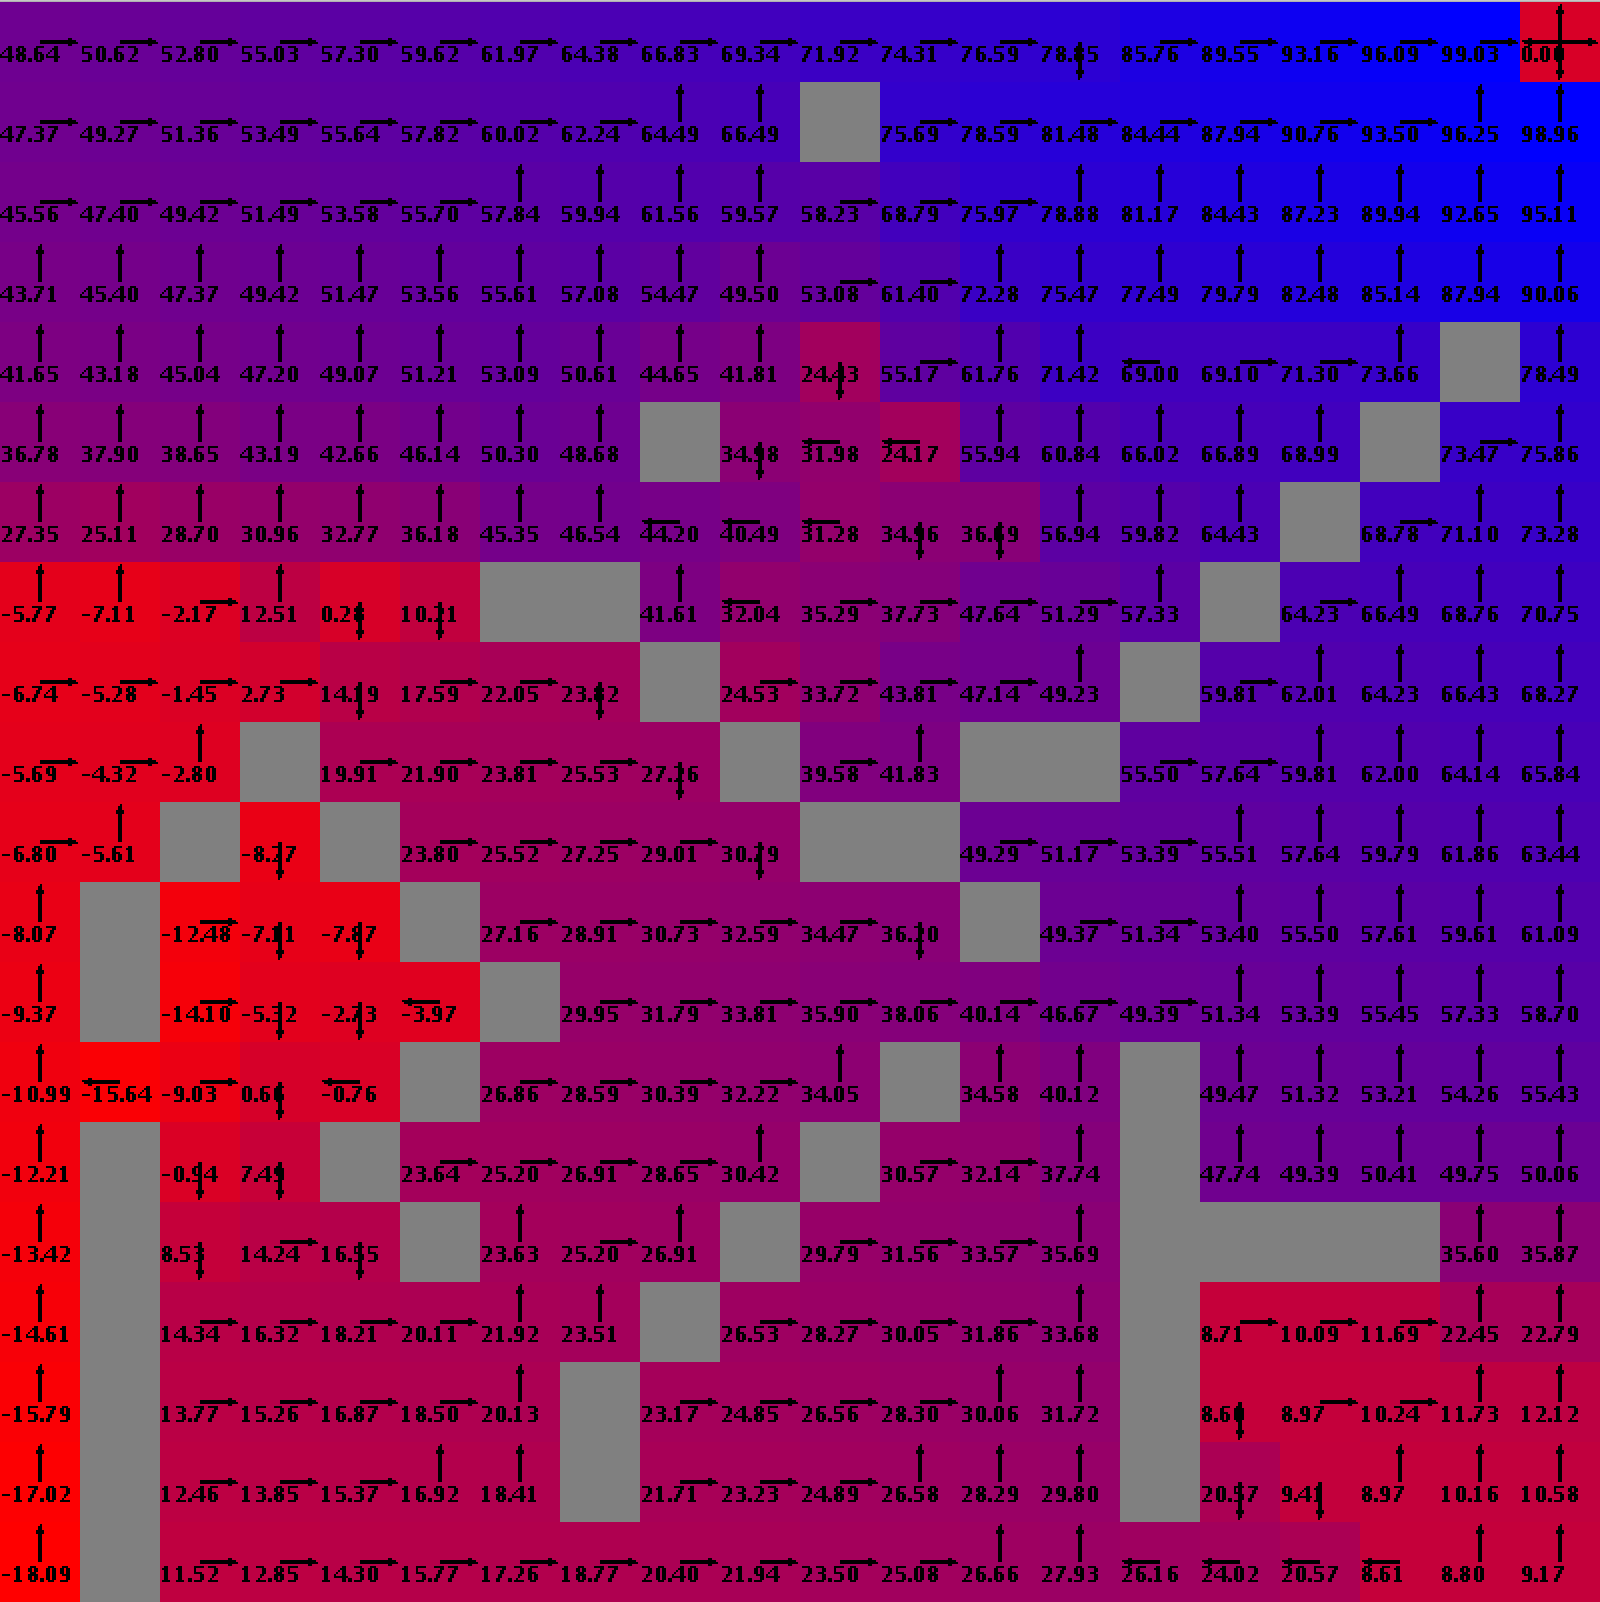
\includegraphics[width=1\textwidth,keepaspectratio]{hard-policy-10.png} 
      \caption*{Hard GW Policy Iteration \#10} 
   \endminipage\hfill
   \minipage{0.245\textwidth}
      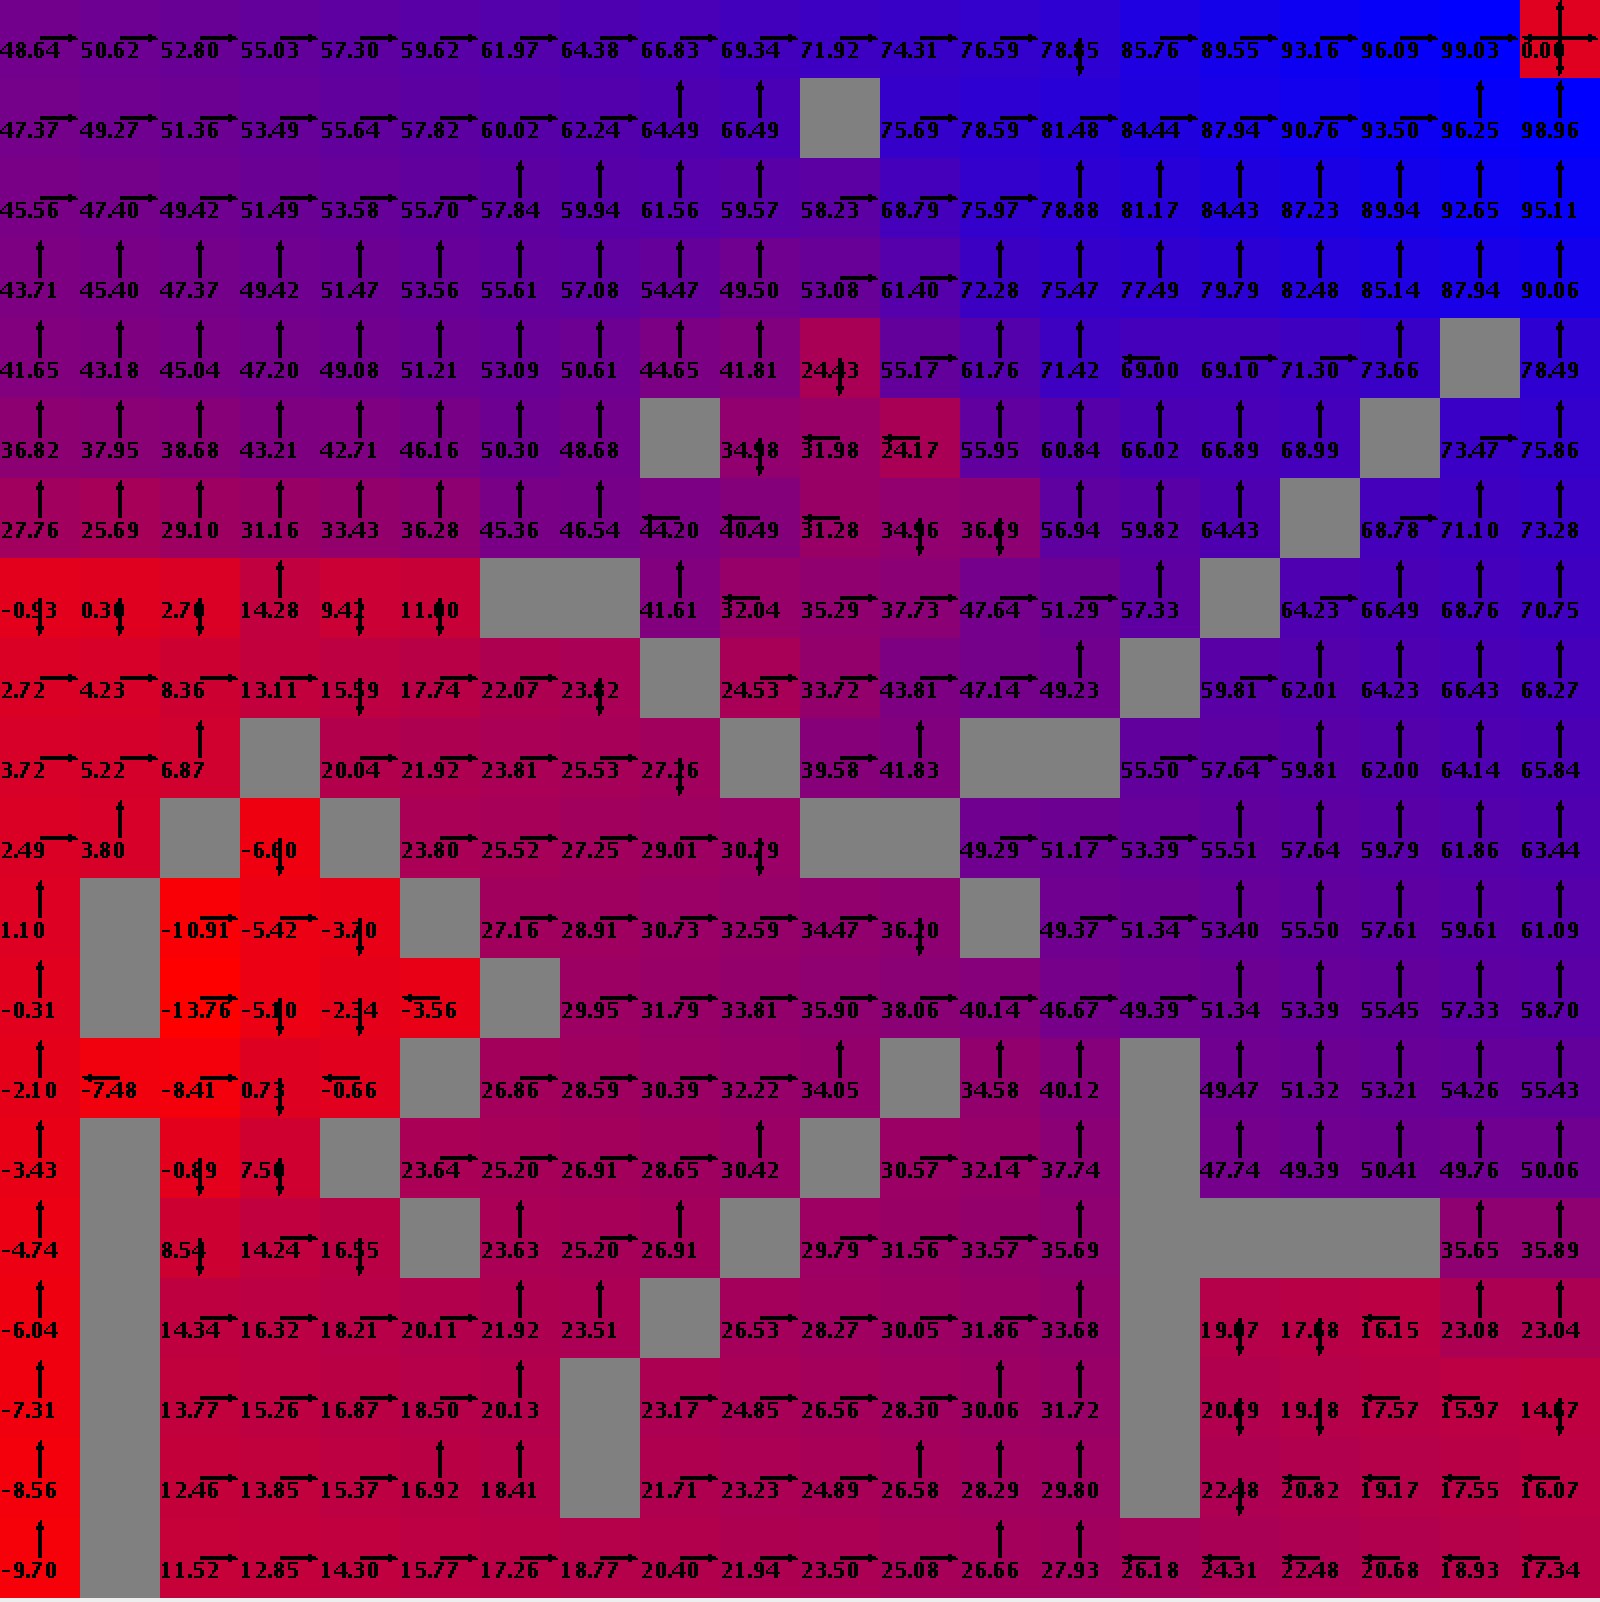
\includegraphics[width=1\textwidth,keepaspectratio]{hard-policy-22.png} 
      \caption*{Hard GW Policy Iteration \#22} 
   \endminipage\hfill
\end{figure}



 
\section*{Q-learning}
\subsection*{Introduction}
The third reinforcement algorithm used to optimally solve the MDPs is 
Q-learning.  Q-learning works by assigning q values to every state.  At each state, the learner calculates new 
q values based on both immediate and future rewards.  Initially, Q-learning will 
spend time exploring and learning, whereas it will eventually optimize
based on knowledge learned and converge.  While the first two algorithms have domain knowledge about the problem, 
Q-learning has no such information and learns as it goes. 


\begin{figure}[H] 
\centering
\begin{tabular}{ | c | c  | c | c | c | c | c | c| c| c| c| c| c | } 
\hline
\textbf{ Q-learning Params } & \textbf{Iterations} & \textbf{Time} & \textbf{Reward} & \textbf{Steps} & \textbf{Convergence}   \\
\hline
\textbf{EASY Gridworld} \\ \hline
\textbf{L0.1 q0.0 E0.1} & 158 & 0.0896 & 50.4200 & 47.9200 & 5.3800 \\ \hline
\textbf{L0.9 q100.0 E0.3} & 294 & 0.0571 & 49.9600 & 48.4200 & 21.9495 \\ \hline
\textbf{L0.9 q0.0 E0.3} & 156 & 0.0416 & 48.4000 & 47.4000 & 53.3545 \\ \hline
\textbf{L0.9 q0.0 E0.5} & 19 & 0.0093 & 45.9200 & 50.9800 & 63.1121 \\ \hline
\textbf{L0.9 q100.0 E0.5} & 615 & 0.1257 & 44.5200 & 47.1200 & 25.2423 \\ \hline
\textbf{L0.9 q100.0 E0.1} & 372 & 0.0806 & 44.0600 & 48.4800 & 22.5748 \\ \hline
\textbf{L0.9 q0.0 E0.1} & 902 & 0.1461 & 43.7200 & 25.2200 & 26.0067 \\ \hline
\textbf{L0.9 q-100.0 E0.5} & 880 & 0.1724 & 43.6400 & 25.3000 & 26.0176 \\ \hline
\textbf{L0.1 q100.0 E0.1} & 210 & 0.0940 & 42.3800 & 52.1000 & 0.6710 \\ \hline
\textbf{L0.1 q0.0 E0.3} & 936 & 0.1276 & 41.8000 & 25.2200 & 3.5595 \\ \hline
\hline
\\
\textbf{HARD Gridworld} \\ \hline
\textbf{L0.1 q0.0 E0.1} & 2900 & 0.8542 & 19.6100 & 63.7700 & 2.1298 \\ \hline
\textbf{L0.1 q100.0 E0.5} & 1882 & 0.8056 & 19.5100 & 63.8700 & 1.3662 \\ \hline
\textbf{L0.1 q0.0 E0.3} & 2411 & 0.8169 & 19.0300 & 64.1900 & 2.9960 \\ \hline
\textbf{L0.1 q0.0 E0.5} & 1177 & 0.5065 & 18.9700 & 62.9800 & 3.6562 \\ \hline
\textbf{L0.1 q100.0 E0.3} & 2958 & 1.0309 & 18.4100 & 64.9200 & 1.8214 \\ \hline
\textbf{L0.1 q100.0 E0.1} & 2685 & 0.9719 & 17.8000 & 63.1300 & 1.7738 \\ \hline
\textbf{L0.9 q0.0 E0.3} & 1728 & 0.9165 & 5.7800 & 70.0500 & 64.5125 \\ \hline
\textbf{L0.9 q0.0 E0.1} & 754 & 0.4340 & -15.2900 & 63.1400 & 46.8360 \\ \hline
\textbf{L0.9 q100.0 E0.5} & 1891 & 0.9692 & -17.2500 & 89.3400 & 40.4389 \\ \hline
\textbf{L0.9 q100.0 E0.1} & 2791 & 1.4653 & -19.1800 & 62.6200 & 42.1840 \\ 
\hline
\end{tabular}
\caption*{Gridworld Q-learning results for various parameter configurations, sorted by max reward } 
\end{figure}


 \subsubsection*{Q-Learning Results}
 The results obtained using Q-learning on the gridworld problems were quite 
 interesting.  Unlike the policy and value iterations, Q-learning knows nothing 
 about the model and learns as it explores.  
 \\ \\ 
 A variety of parameters were 
 used to tune an optimal learner for each problem.  These parameters included the
 learning rate, the intial q value to be set, and the epsilon 
 parameter for the greedy method of selecting from available actions.  In a follow-up excercise, it would be worthwhile to use other decision policies 
 than Epsilon Greedy policy.  For each 
 trial, a maximum number of steps to explore for each learning episode is defined as 300.  
 A summary of the results from varying these parameters is displayed above.  
 \\ \\
 Interestingly enough, a learning rate of 0.1, initial q values of 0, and an 
 epsilon value of 0.1 were the optimal parameters for both the easy and hard 
 gridworld problem.  The low q values helped to encourage exploration as they indicated neutral initial information.
 The low learning rate also put an emphasis on older information which is 
 helpful in navigating a maze succesfully.
 The number of iterations and time, however, varied greatly.  
 \\ \\
 For the easy gridworld problem, the optimal results took 158 iterations to 
 achieve a maximum reward as well as meet a somewhat low convergence factor.  
 These results were very similar to the ones observed from the previous policy and 
 value iterations.  Interestingly, the time to run the algorithm was even 
 faster.  This can be attributed to the q-learning algorithm not wasting its 
 time exploring bad worthless paths as it progresses.  A lower learning rate 
 also helps to make sure it utilizes information about valuable paths.
 \\ \\
 For the hard gridworld problem, the optimal result took a much longer 2900 
 iterations.  As the learner had to explore and navigate a fairly complex maze, 
 this makes sense.  From the policy maps below, it's clear that the algorithm 
 develops an optimal path that it tries to follow barring randomly choosing a 
 wrong direction.  Again, its run time was quite low compared to the other 
 approaches for solving the MDP.  Reasonably, the hard gridworld q-learner takes 
 longer to run than the easy gridworld q-learner. 


    \begin{figure}[H]
  \minipage{0.245\textwidth}
      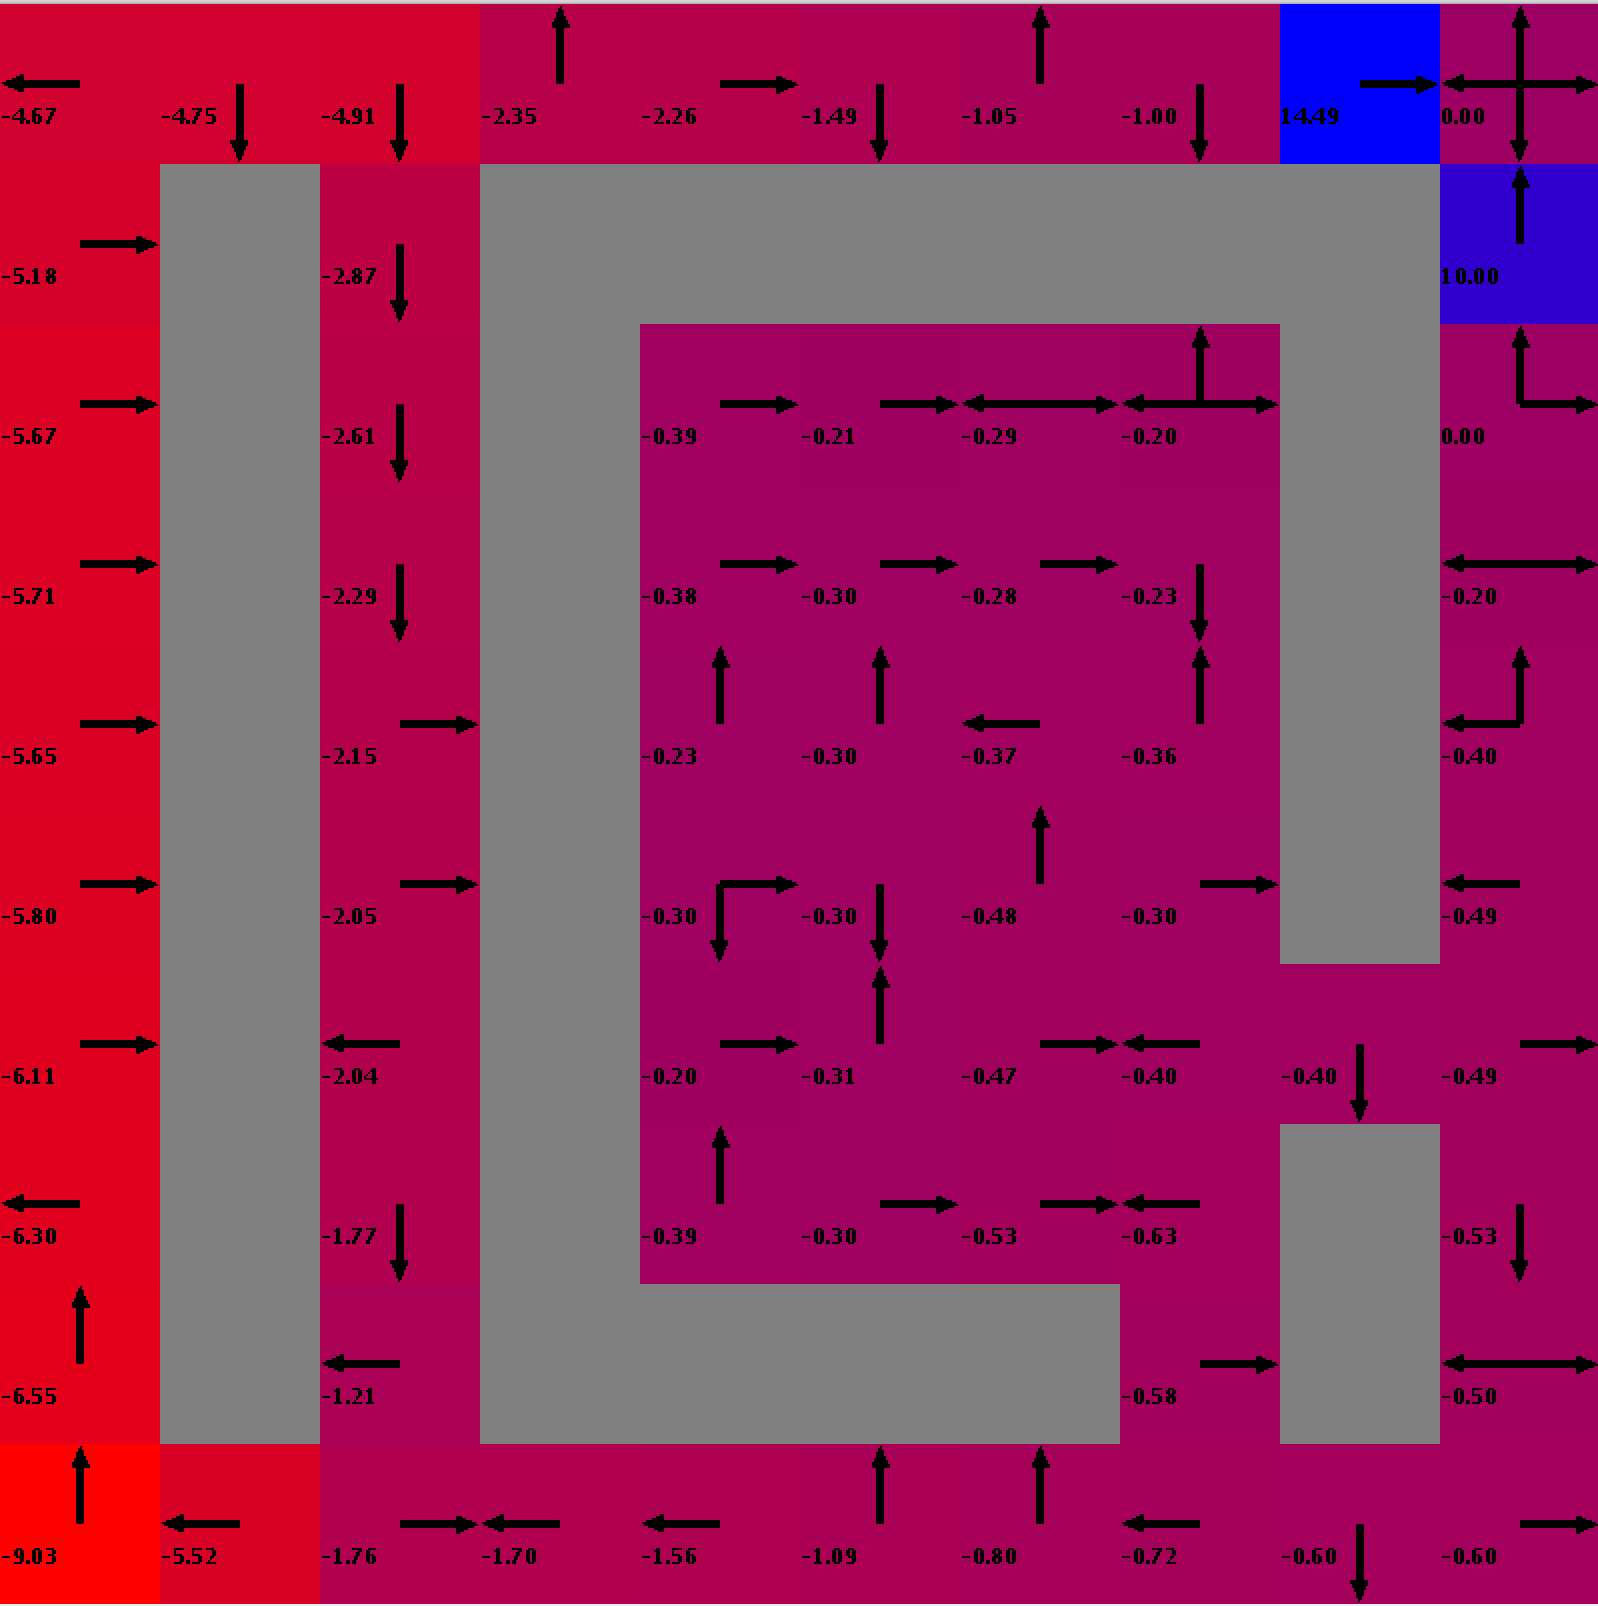
\includegraphics[width=1\textwidth,keepaspectratio]{easy-q-8.png} 
      \caption*{Easy GW Q-learning Iteration \#8} 
   \endminipage\hfill
   \minipage{0.245\textwidth}
      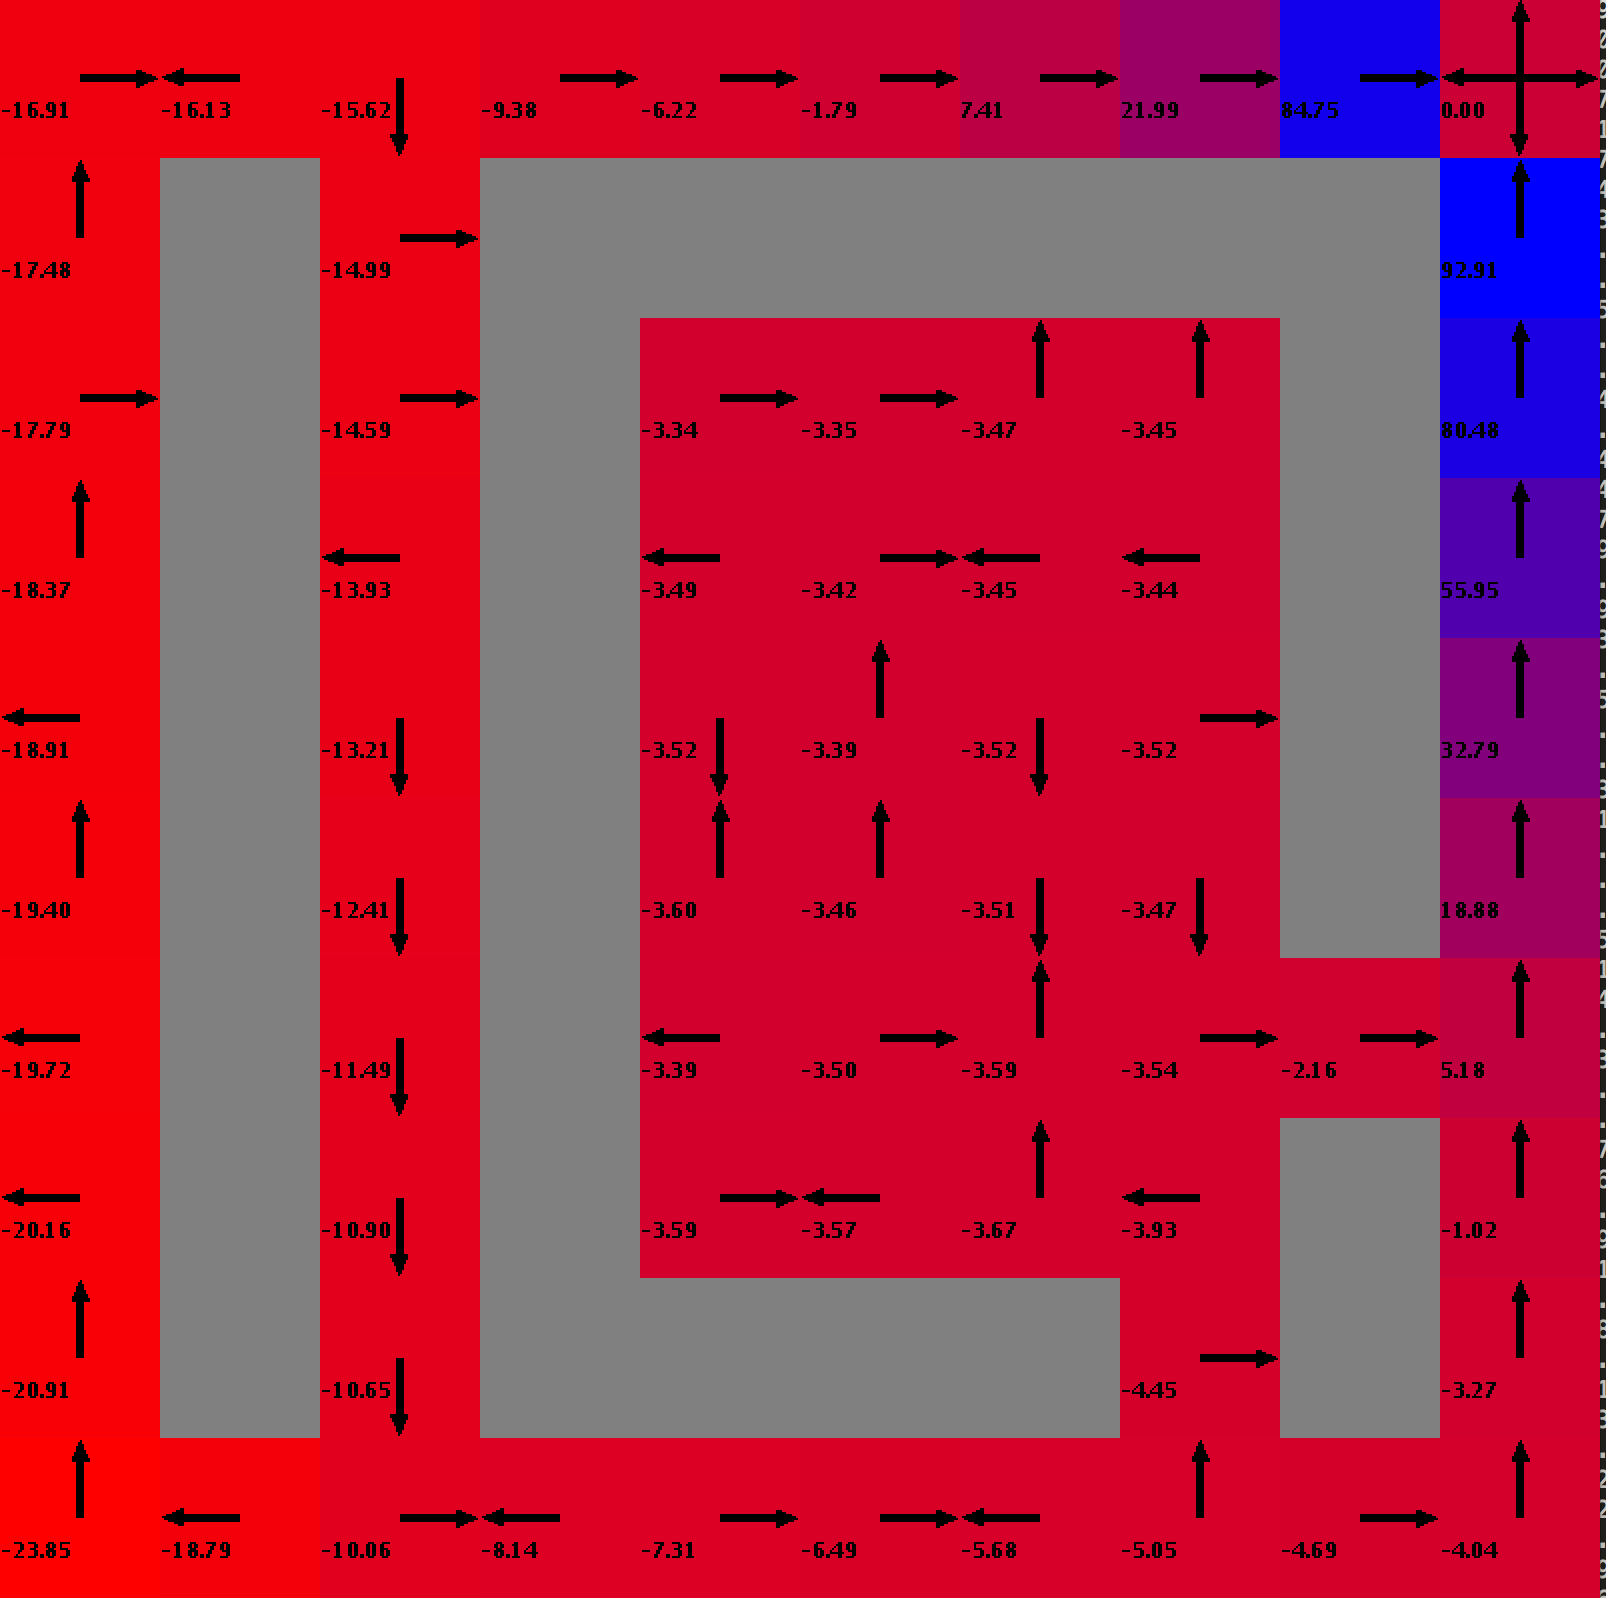
\includegraphics[width=1\textwidth,keepaspectratio]{easy-q-50.png} 
      \caption*{Easy GW Q-learning Iteration \#50} 
   \endminipage\hfill
   \minipage{0.245\textwidth}
      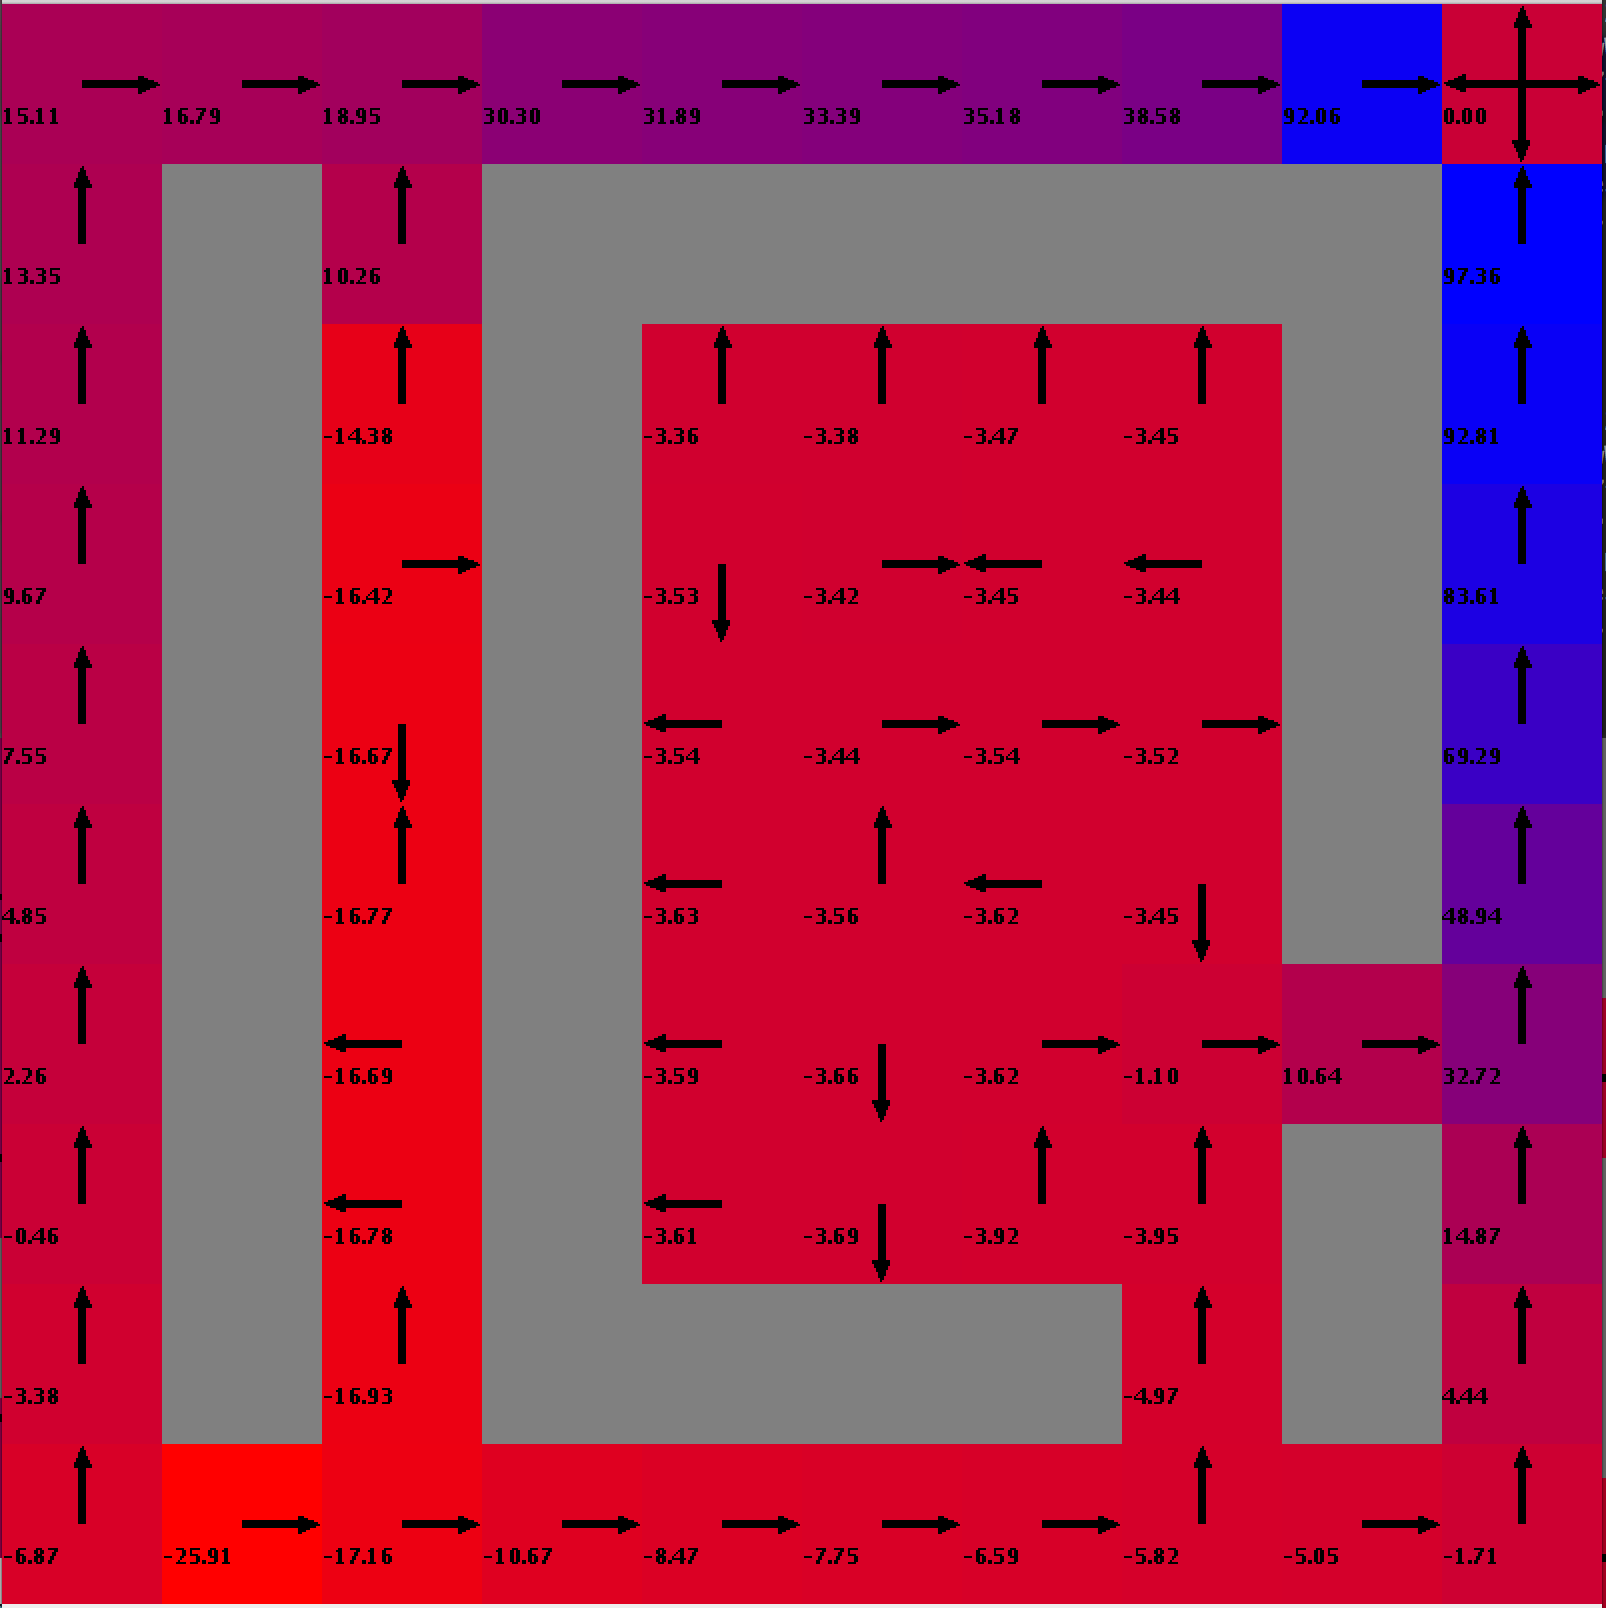
\includegraphics[width=1\textwidth,keepaspectratio]{easy-q-158.png} 
      \caption*{Easy GW Q-learning Iteration \#158} 
   \endminipage\hfill
   \minipage{0.245\textwidth}
      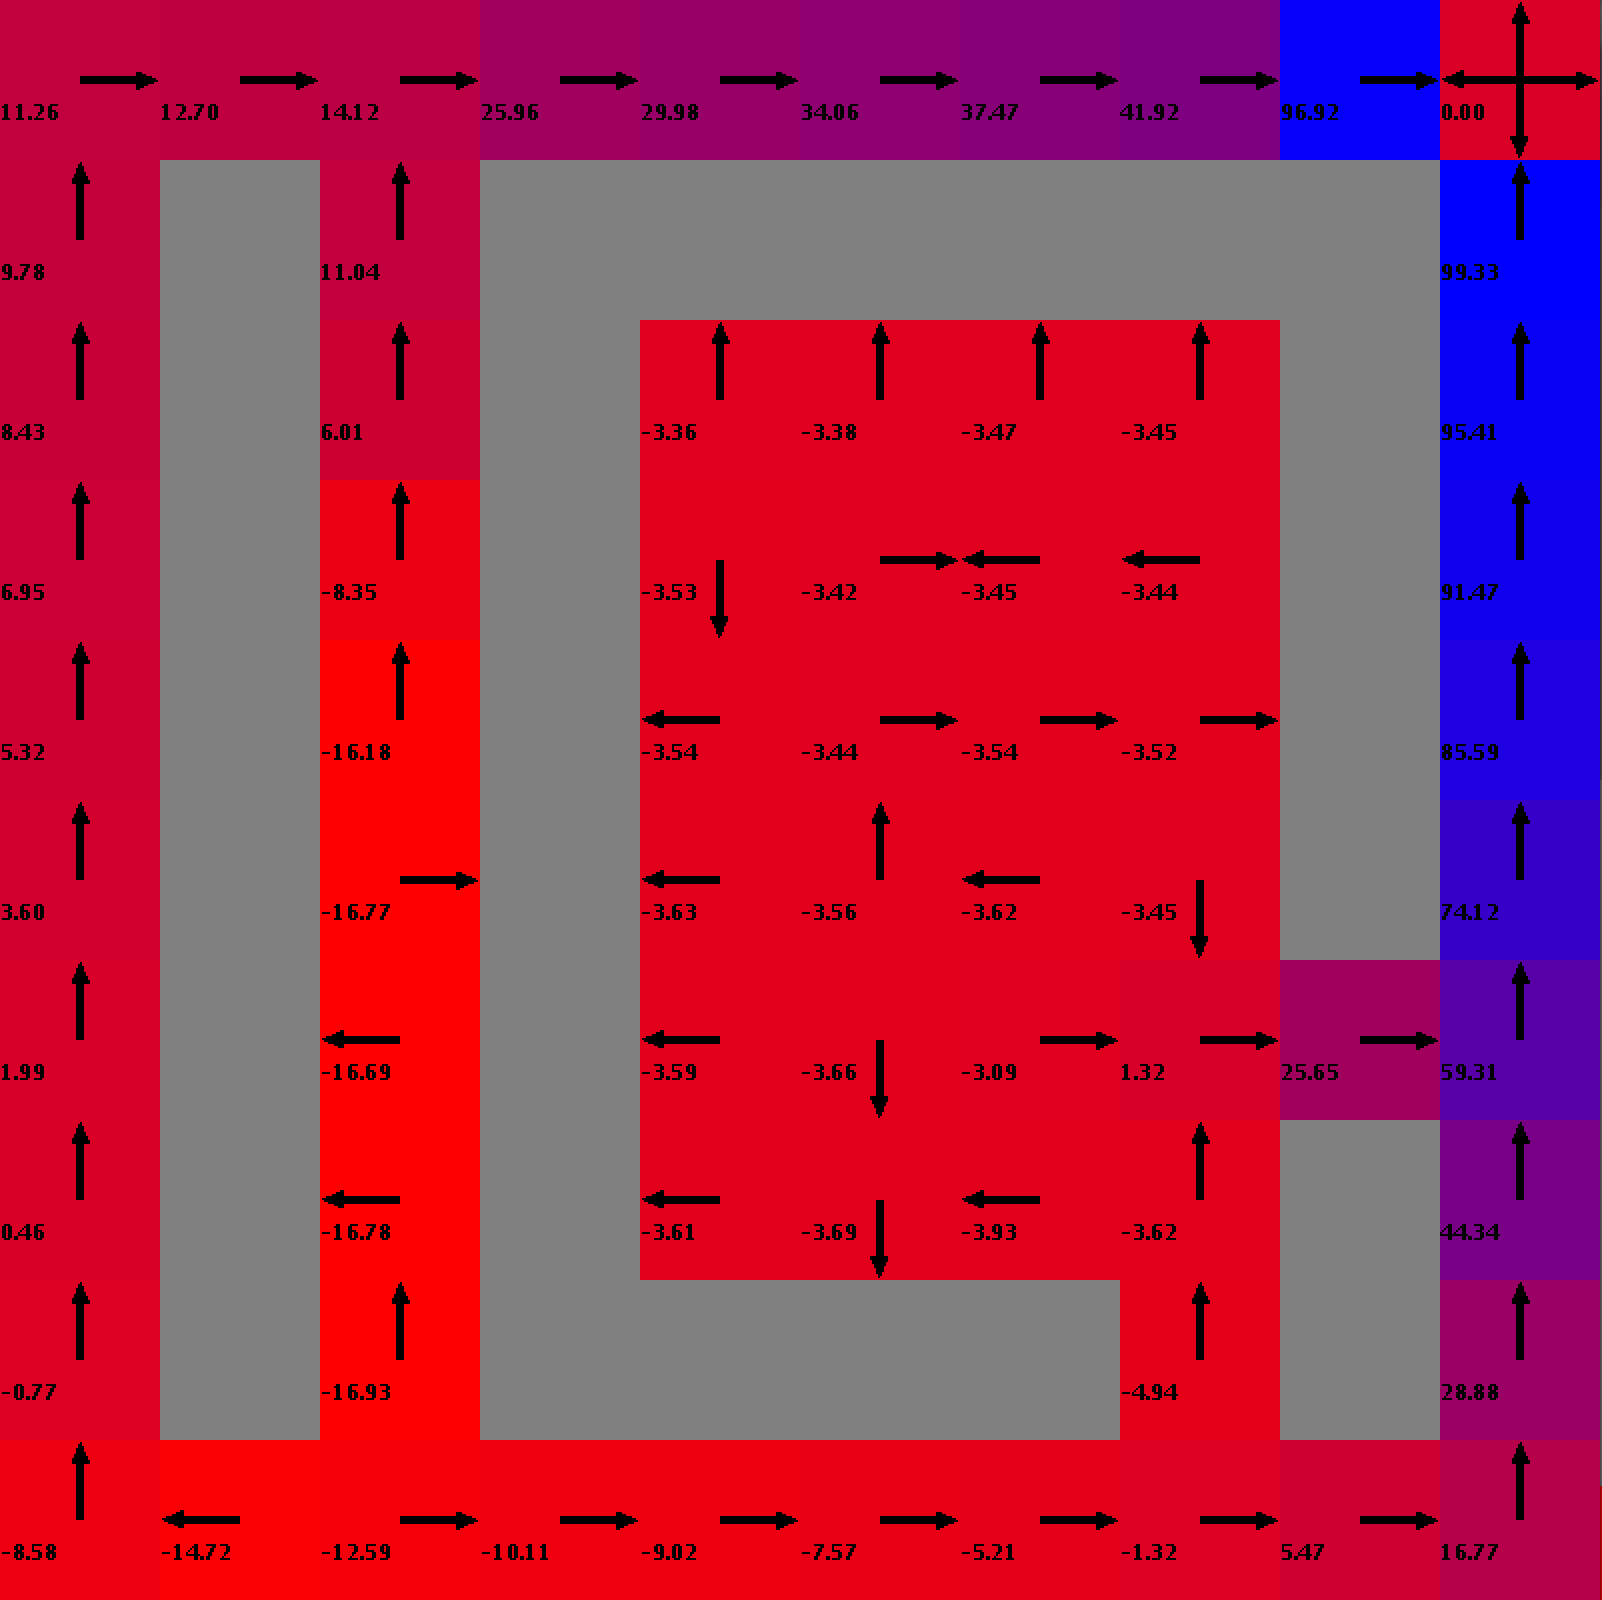
\includegraphics[width=1\textwidth,keepaspectratio]{easy-q-1000.png} 
      \caption*{Easy GW Q-learning Iteration \#1000} 
   \endminipage\hfill
\end{figure}

   \begin{figure}[H]
  \minipage{0.245\textwidth}
      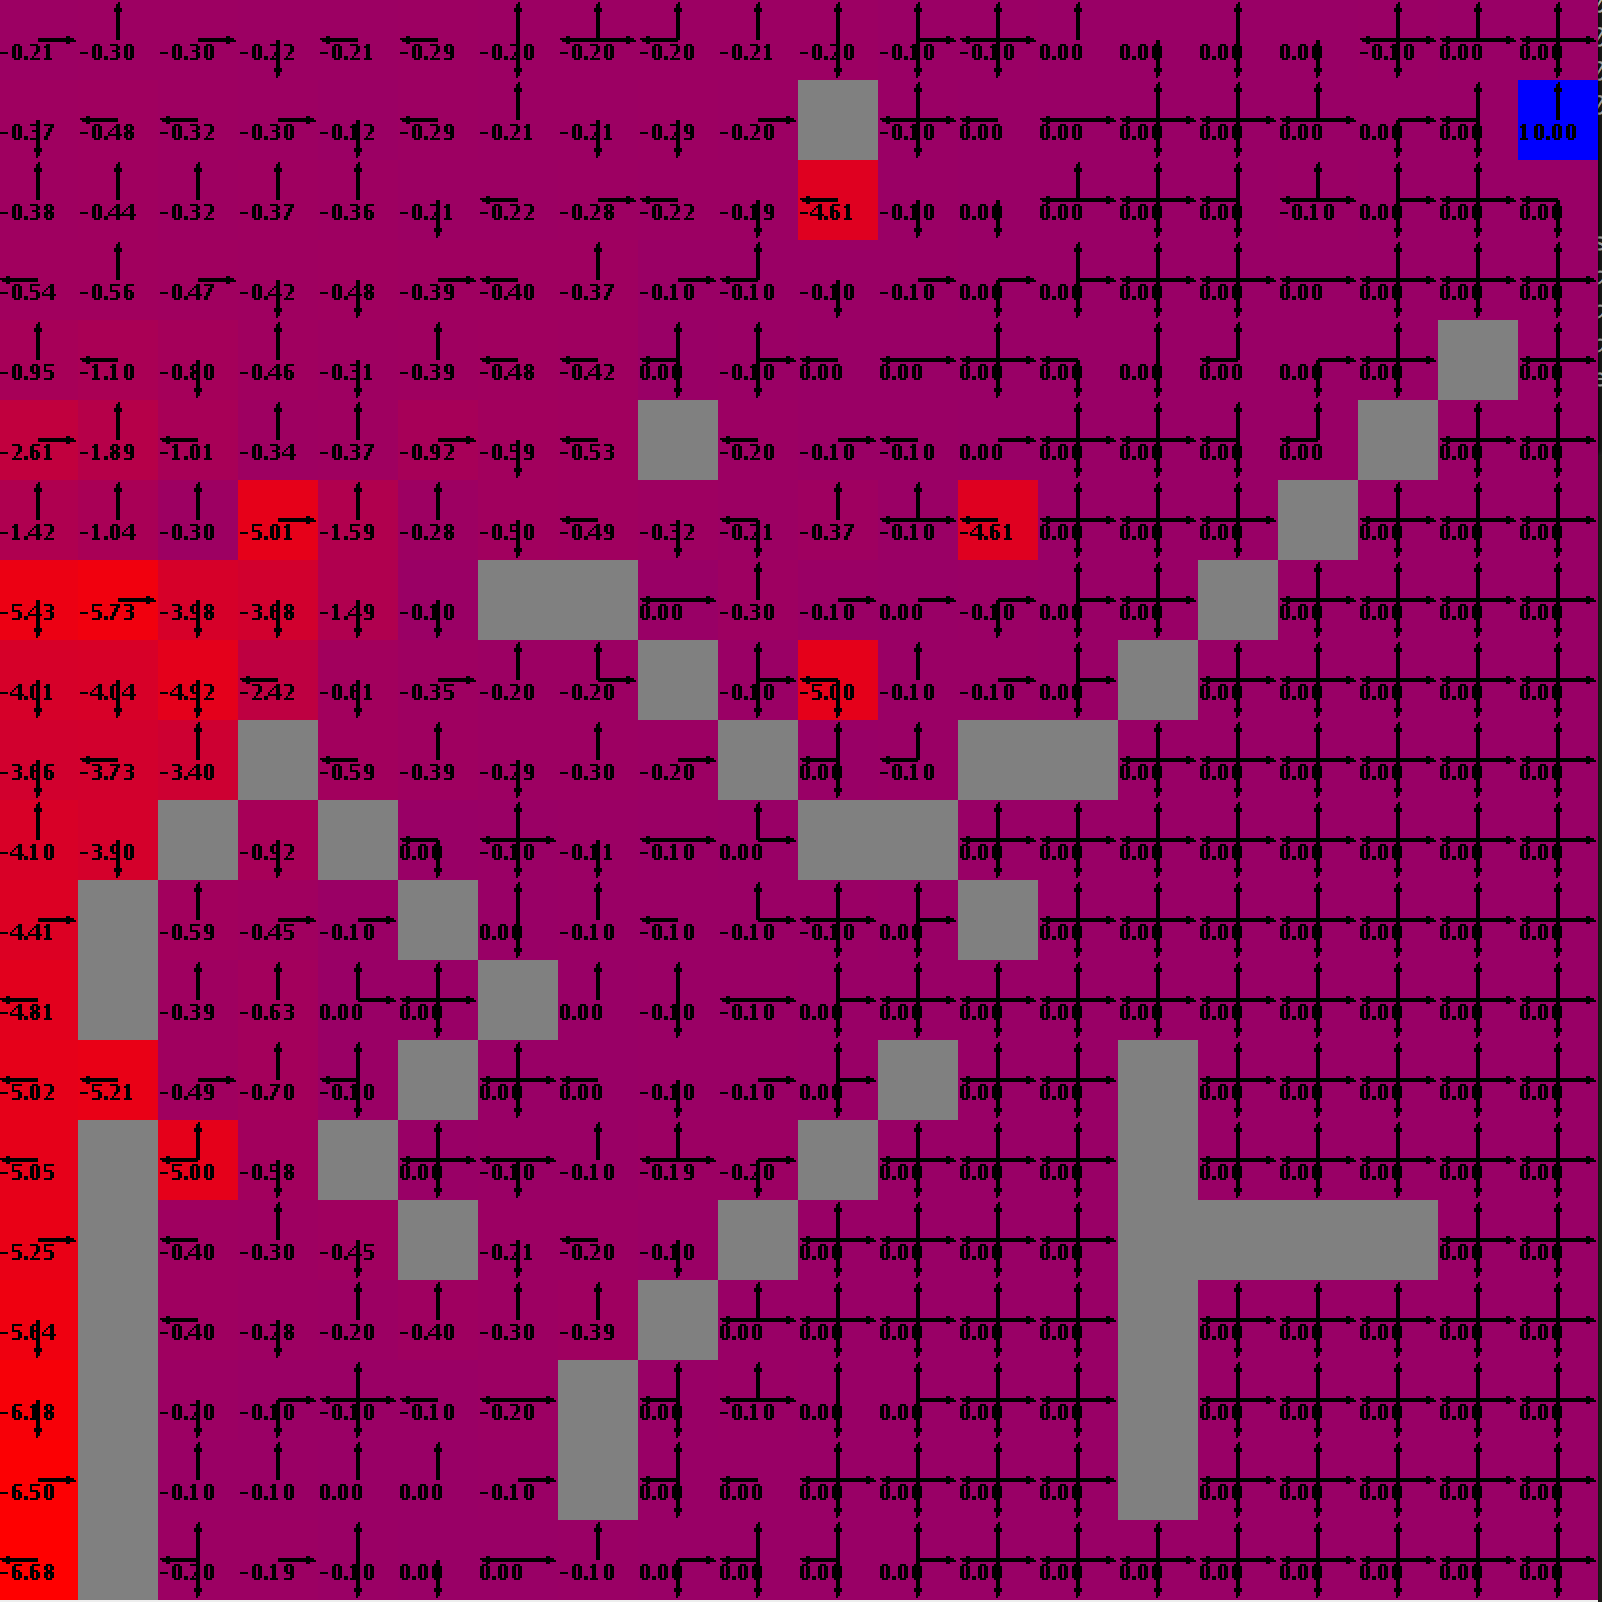
\includegraphics[width=1\textwidth,keepaspectratio]{hard-q-9.png} 
      \caption*{Hard GW Q-learning Iteration \#9} 
   \endminipage\hfill
   \minipage{0.245\textwidth}
      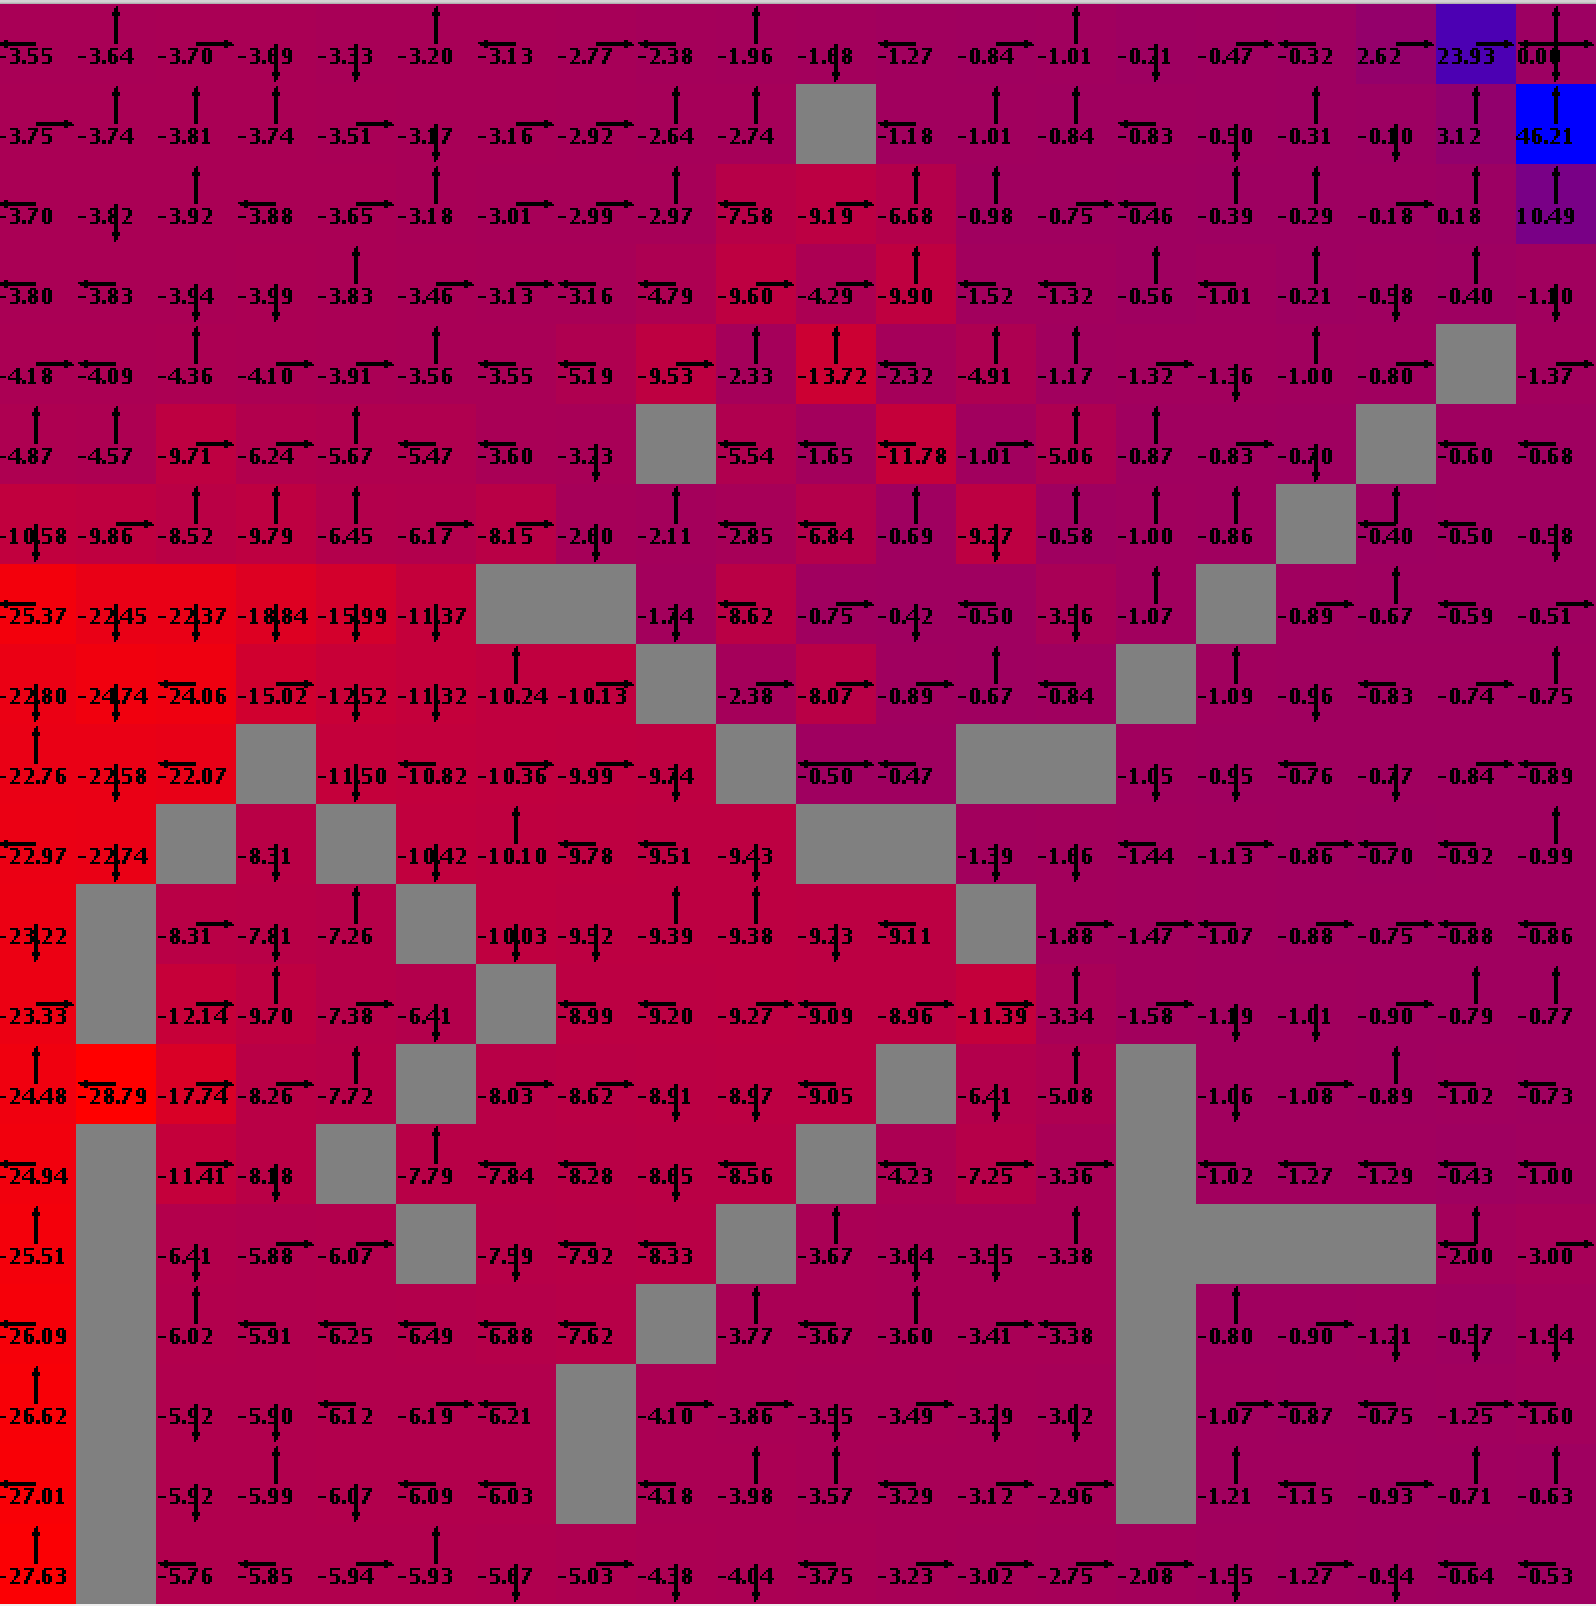
\includegraphics[width=1\textwidth,keepaspectratio]{hard-q-100.png} 
      \caption*{Hard GW Q-learning Iteration \#100} 
   \endminipage\hfill
   \minipage{0.245\textwidth}
      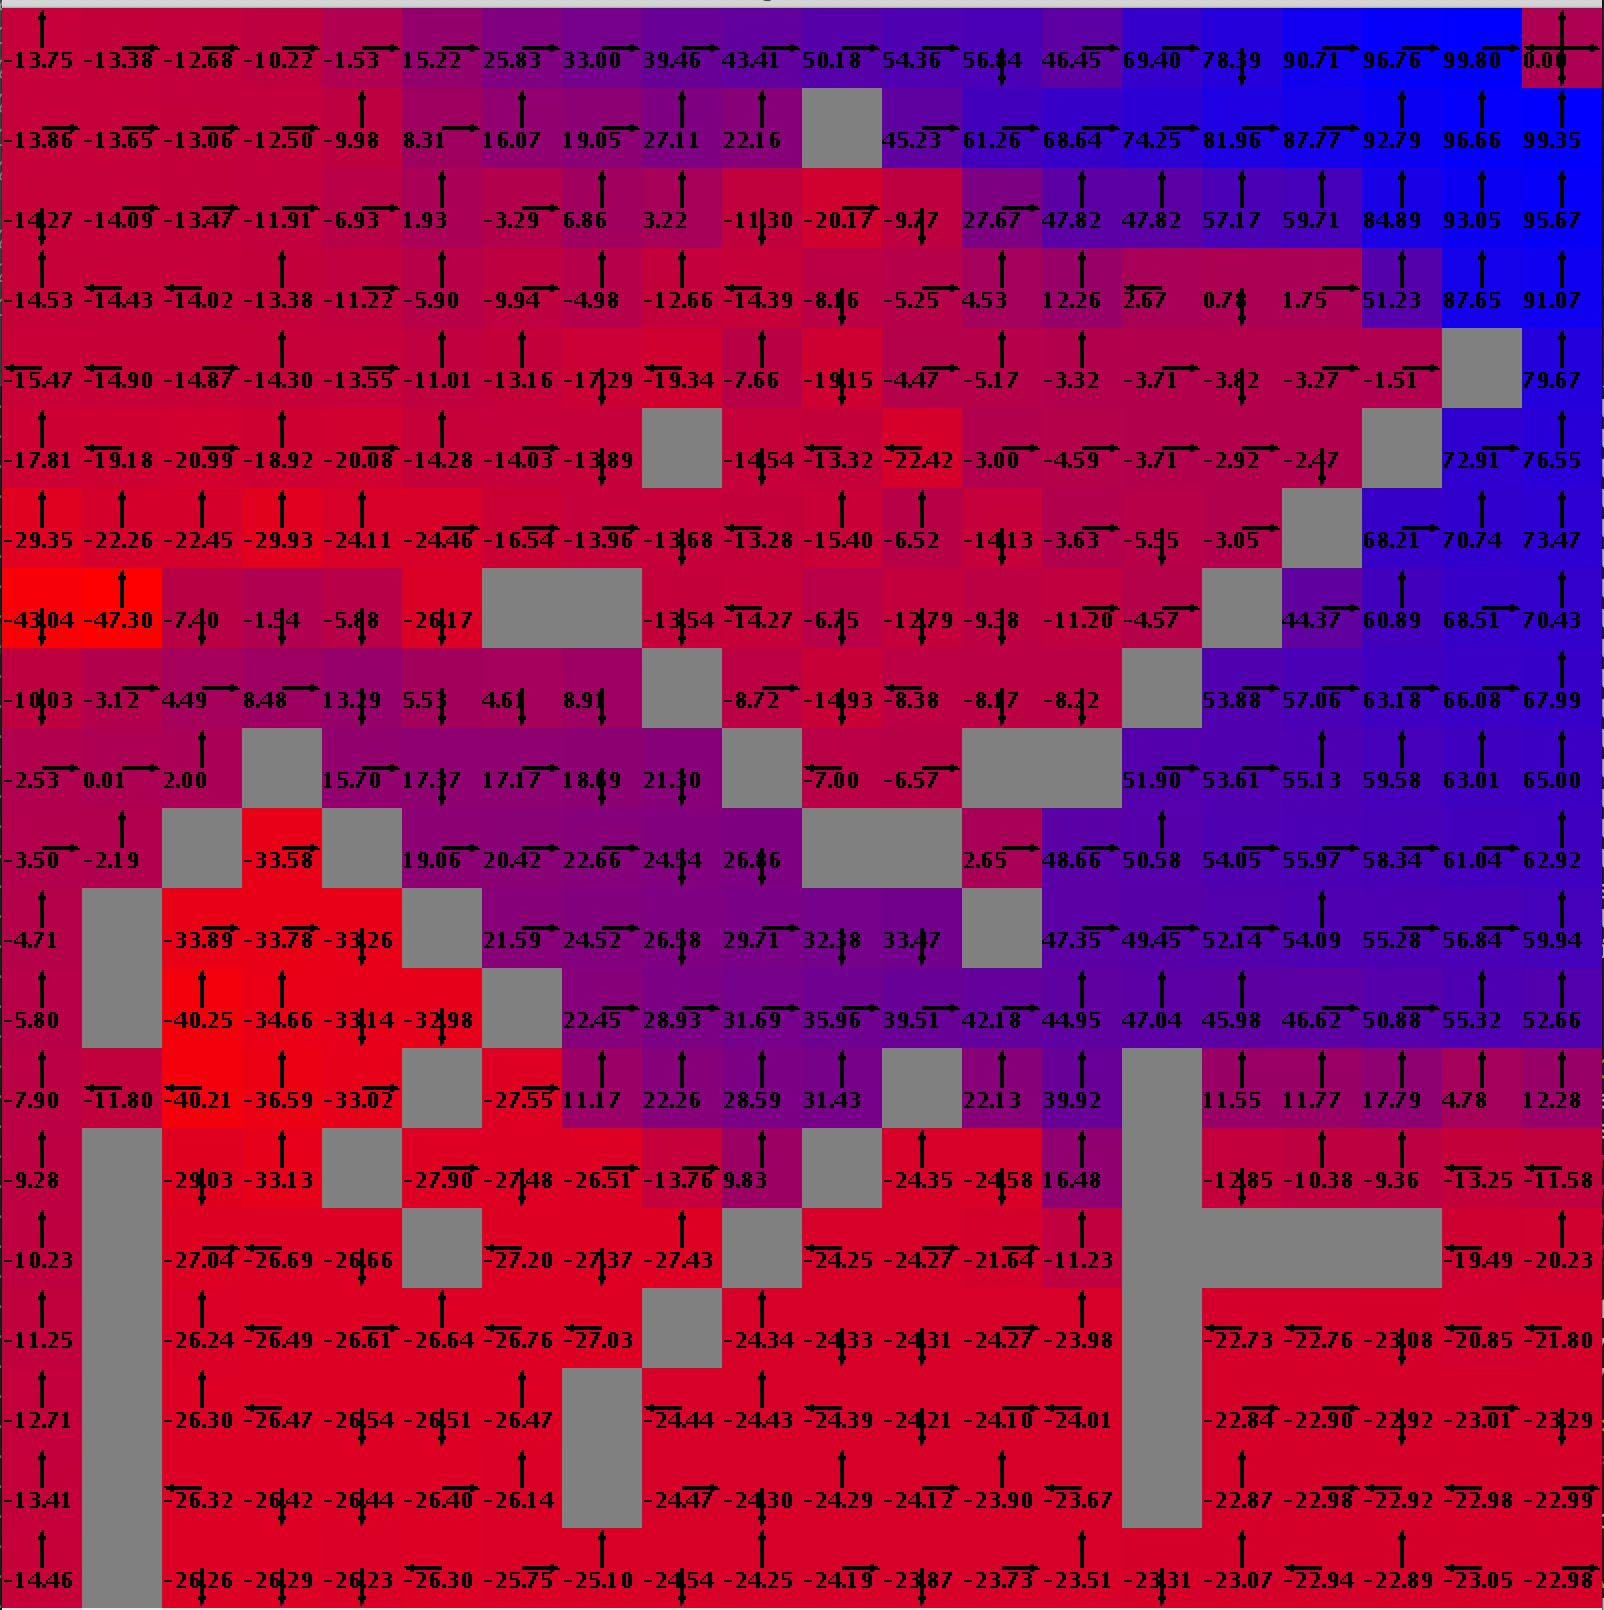
\includegraphics[width=1\textwidth,keepaspectratio]{hard-q-1066.png} 
      \caption*{Hard GW Q-learning Iteration \#1066} 
   \endminipage\hfill
   \minipage{0.245\textwidth}
      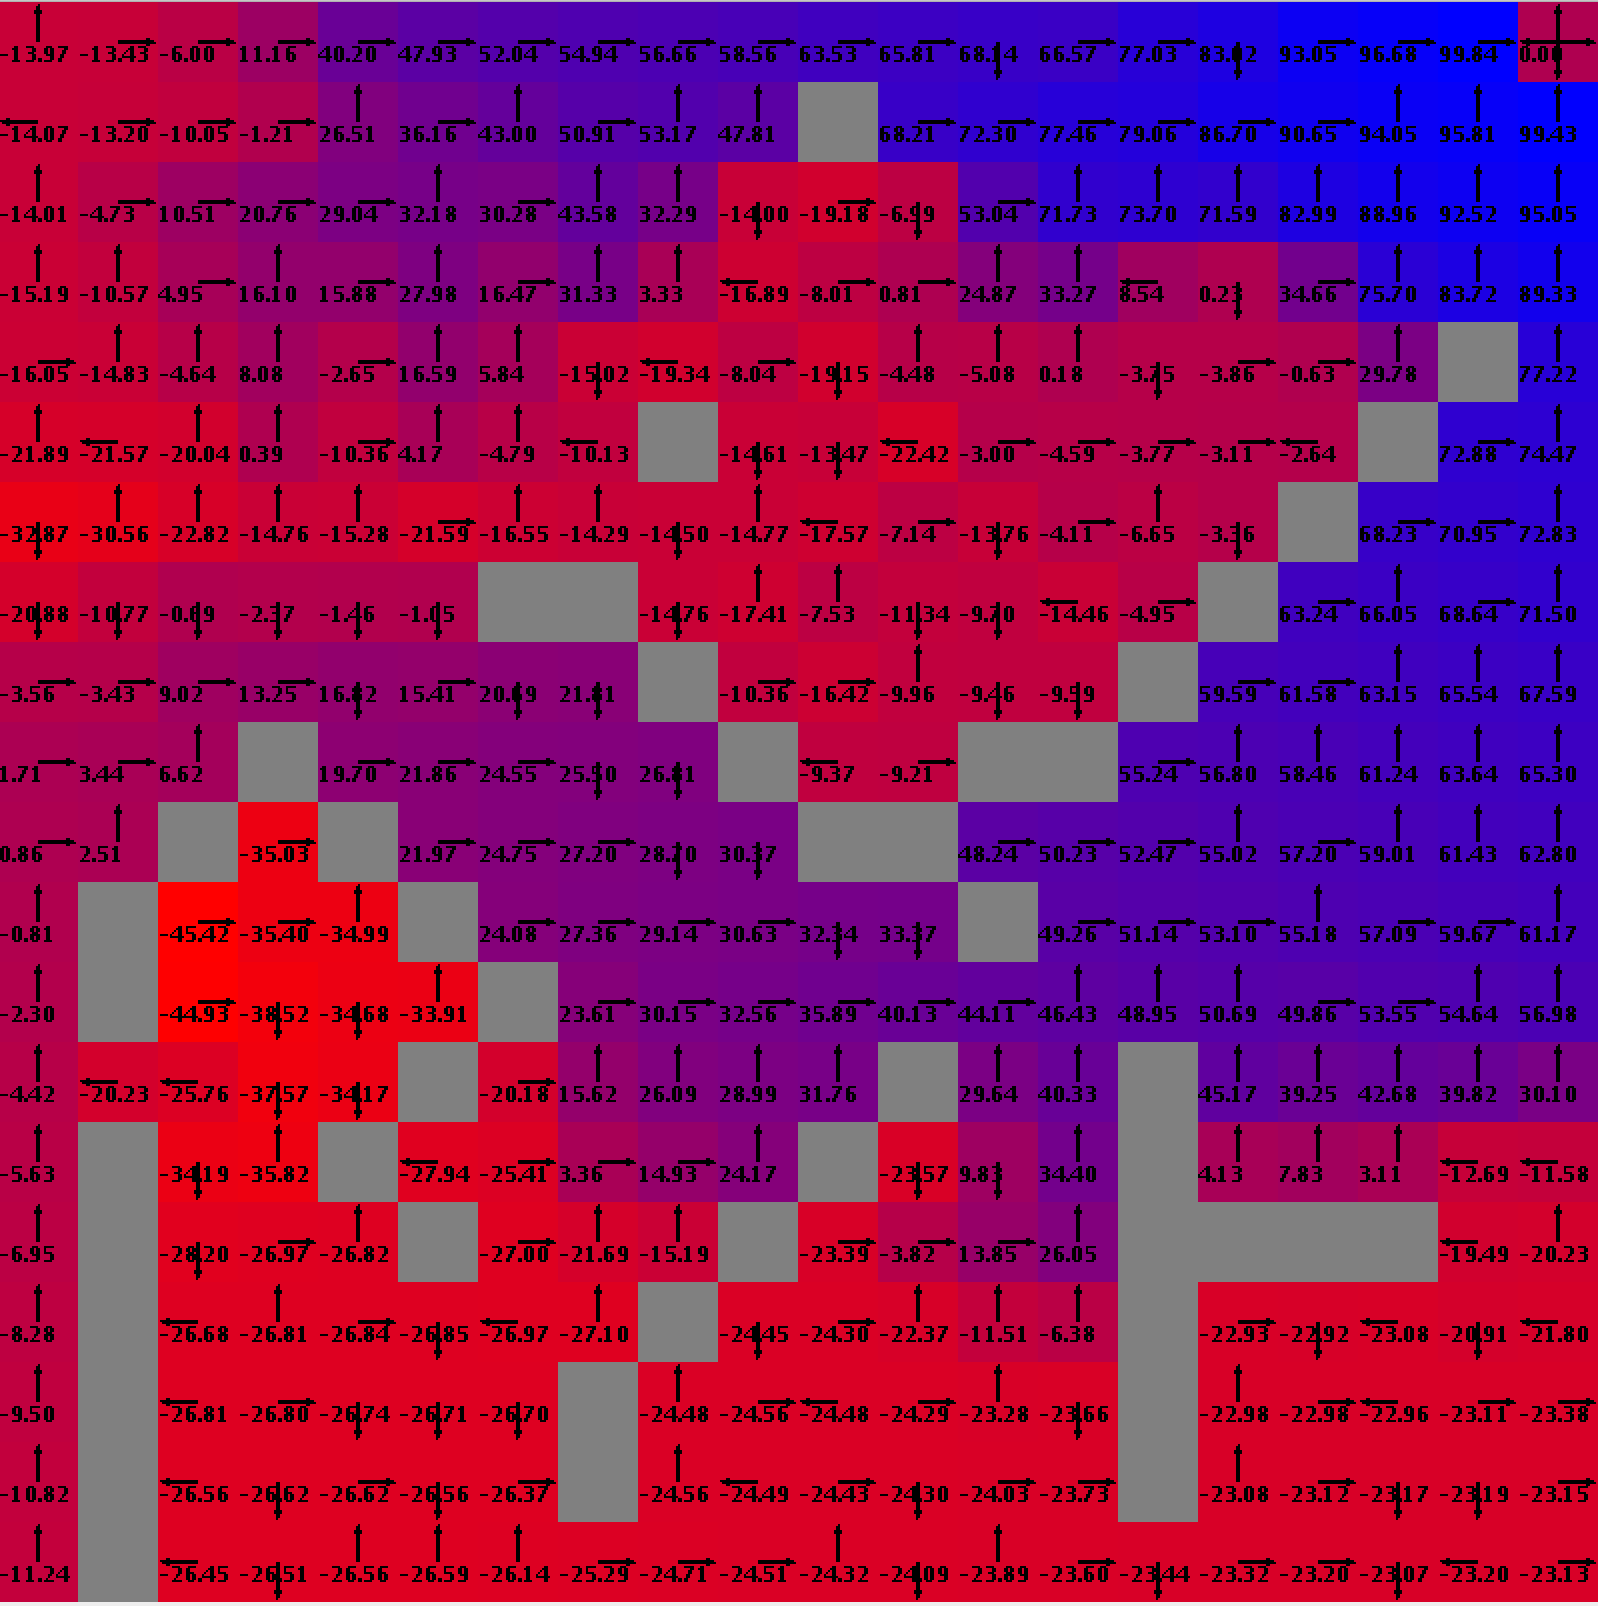
\includegraphics[width=1\textwidth,keepaspectratio]{hard-q-2900.png} 
      \caption*{Hard GW Q-learning Iteration \#2900} 
   \endminipage\hfill
\end{figure}


\section*{Algorithm Comparisons}

  \begin{figure}[H]
  \minipage{0.01\textwidth}
   \endminipage\hfill
  \minipage{0.49\textwidth}
      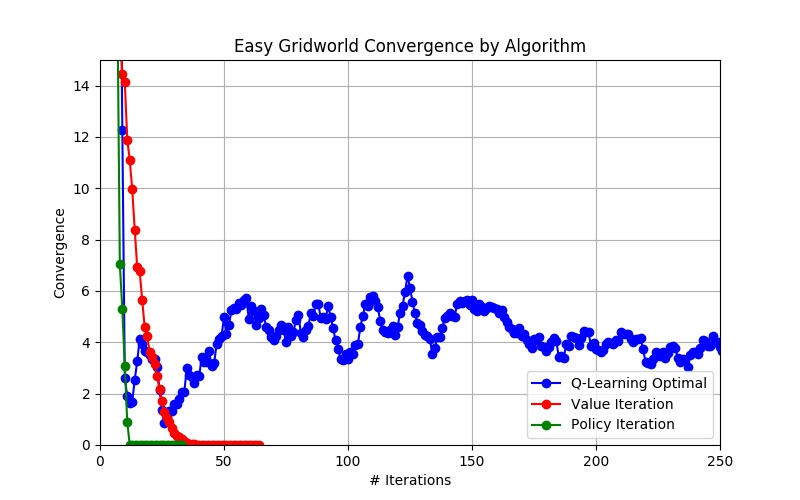
\includegraphics[width=1\textwidth,keepaspectratio]{easy_convergence.jpg} 
      \caption*{10x10 Easy Gridworld Convergence Comparison} 
   \endminipage\hfill
   \minipage{0.49\textwidth}
      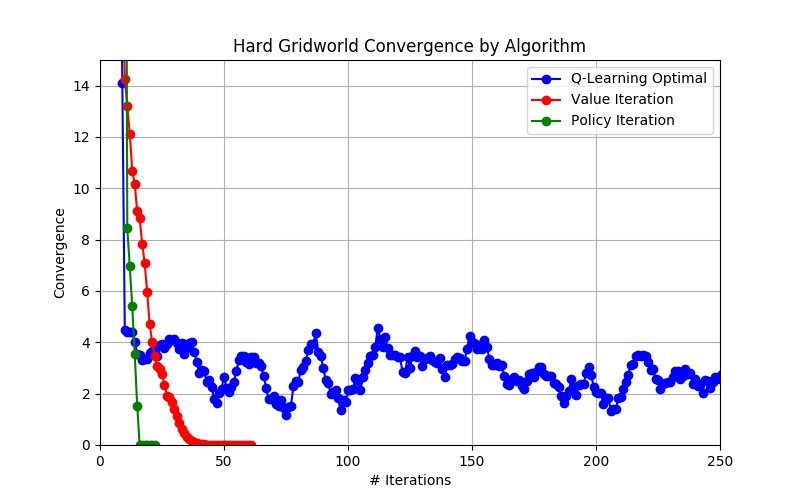
\includegraphics[width=1\textwidth,keepaspectratio]{hard_convergence.jpg} 
      \caption*{20x20 Hard Gridworld Convergence Comparison} 
   \endminipage\hfill
   \minipage{0.01\textwidth}
   \endminipage\hfill
\end{figure}

When comparing the convergence properties of all 3 algorithms, for both MDP problems, it becomes very 
clear that policy iteration has the easiest time converging.  While value 
iteration comes relatively close to policy iteration, Q-learning has a much more 
difficult time.  \\ \\ 
Since policy iteration starts with a random policy and then 
tweaks it for improvements, it is susceptible to converging quickly due to not 
having much reason to change from it's current state.  Similarly, while value 
iteration works backwards, it develops variations but will inevitably converge 
before long to an optimal solution as it is also aided by knowledge of the 
model.  Q-learning, however, goes in completely blind and has much greater 
difficulty knowing if the policy chosen is optimal.  With various options to 
take at each state, it takes many more iterations to converge.


  \begin{figure}[H]
  \minipage{0.01\textwidth}
   \endminipage\hfill
  \minipage{0.49\textwidth}
      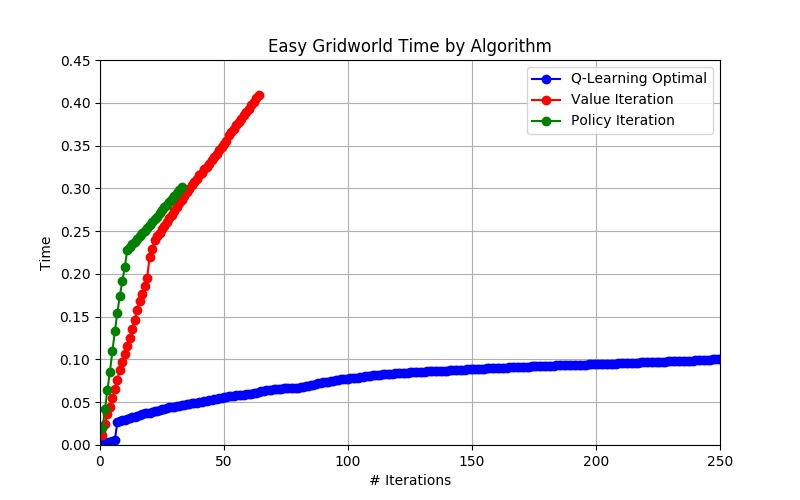
\includegraphics[width=1\textwidth,keepaspectratio]{easy_time.jpg} 
      \caption*{10x10 Easy Gridworld Time Comparison} 
   \endminipage\hfill
   \minipage{0.49\textwidth}
      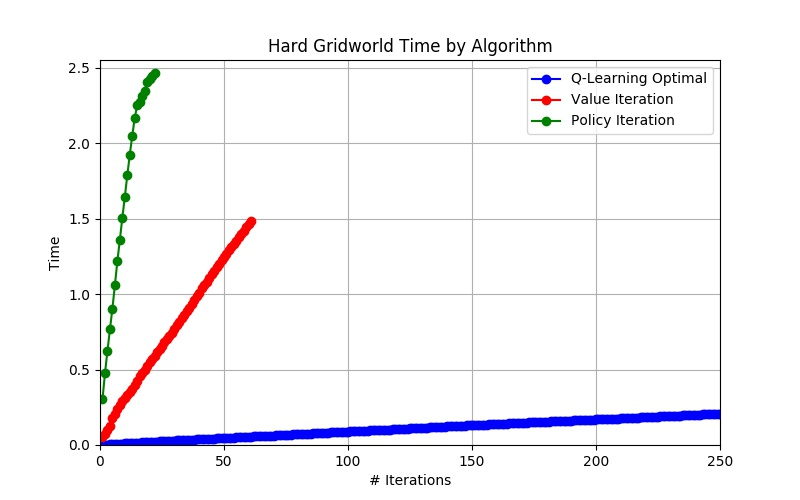
\includegraphics[width=1\textwidth,keepaspectratio]{hard_time.jpg} 
      \caption*{20x20 Hard Gridworld Time Comparison} 
   \endminipage\hfill
   \minipage{0.01\textwidth}
   \endminipage\hfill
\end{figure}
In terms of time necessary to run the algorithm, Q-learning is far and away the 
fastest.  Conversely, policy iteration is the slowest.  Both of these statements 
hold true for both MDPs.  Q-learning does not involve any complex math or 
calculations, unlike policy and value iteration.  Thus, it is able to explore 
and compare its policies much faster than the others.  Q-learning is able to run 
in constant time, whereas value and policy iteration take incrementally more 
time.

  \begin{figure}[H]
  \minipage{0.01\textwidth}
   \endminipage\hfill
  \minipage{0.49\textwidth}
      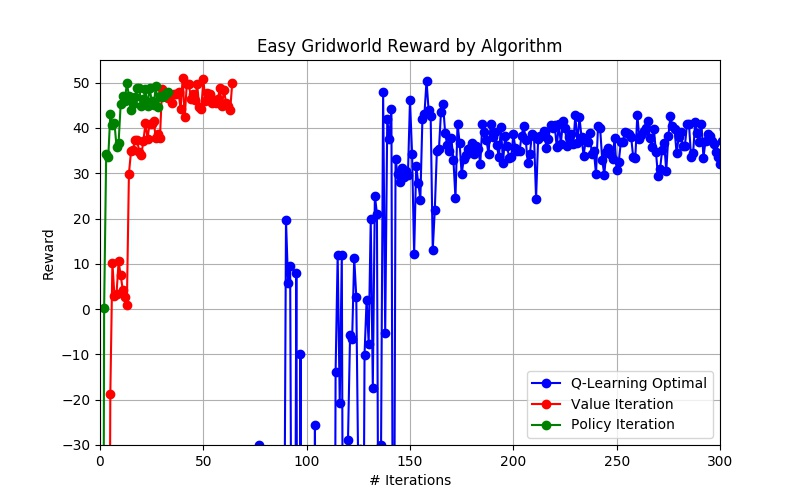
\includegraphics[width=1\textwidth,keepaspectratio]{easy_reward.jpg} 
      \caption*{10x10 Easy Gridworld Reward Comparison} 
   \endminipage\hfill
   \minipage{0.49\textwidth}
      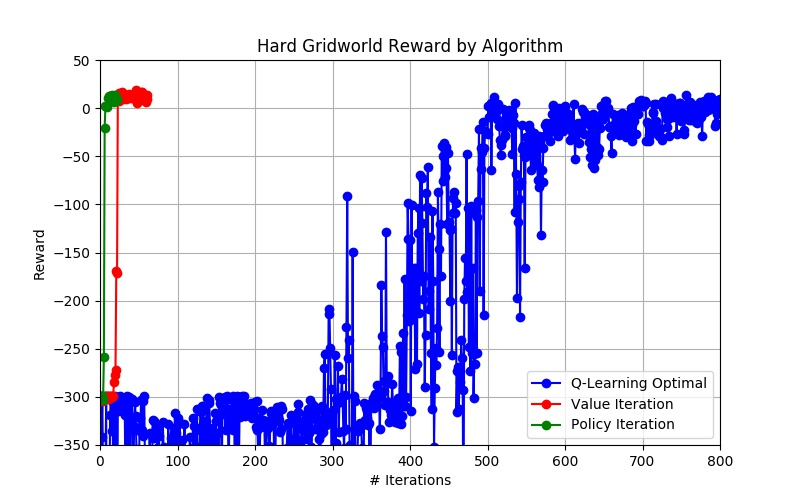
\includegraphics[width=1\textwidth,keepaspectratio]{hard_reward.jpg} 
      \caption*{20x20 Hard Gridworld Reward Comparison} 
   \endminipage\hfill
   \minipage{0.01\textwidth}
   \endminipage\hfill
\end{figure}
Reward analsyis proves to be the most interesting comparison across all three 
algorithms.  Both policy iteration and value iteration were able to find maximal 
rewards quite quickly in terms of iterations, and were able to keep that value 
rather consistent despite thier explorations.  Q-learning, however, struggled 
significantly to find maximal reward polciies, and even once trending towards 
maximal rewards, varied significantly from iteration to iteration.
\\ \\
Policy iteration, having the advantage of making improvement modifications to an 
initial policy, is always seeking to maximize its reward and is thus able to 
almost monotonically increase its reward return while reaching convergence.  
Value iteration is not quite as effective, as it's simply working backwards and 
trying to find good options along the way, but it still performs rather well.  
\\ \\
Q-learning, on the other hand, deals with a large amount of exploration and 
discovery that causes it to take a large number of iterations before it finds 
policies that are able to map to maximal rewards.  Even once it starts 
performing well, it takes a long time to converge and is extremely variable due 
to its tendency to still try to explore new alternatives.


  \begin{figure}[H]
   \minipage{0.32\textwidth}
      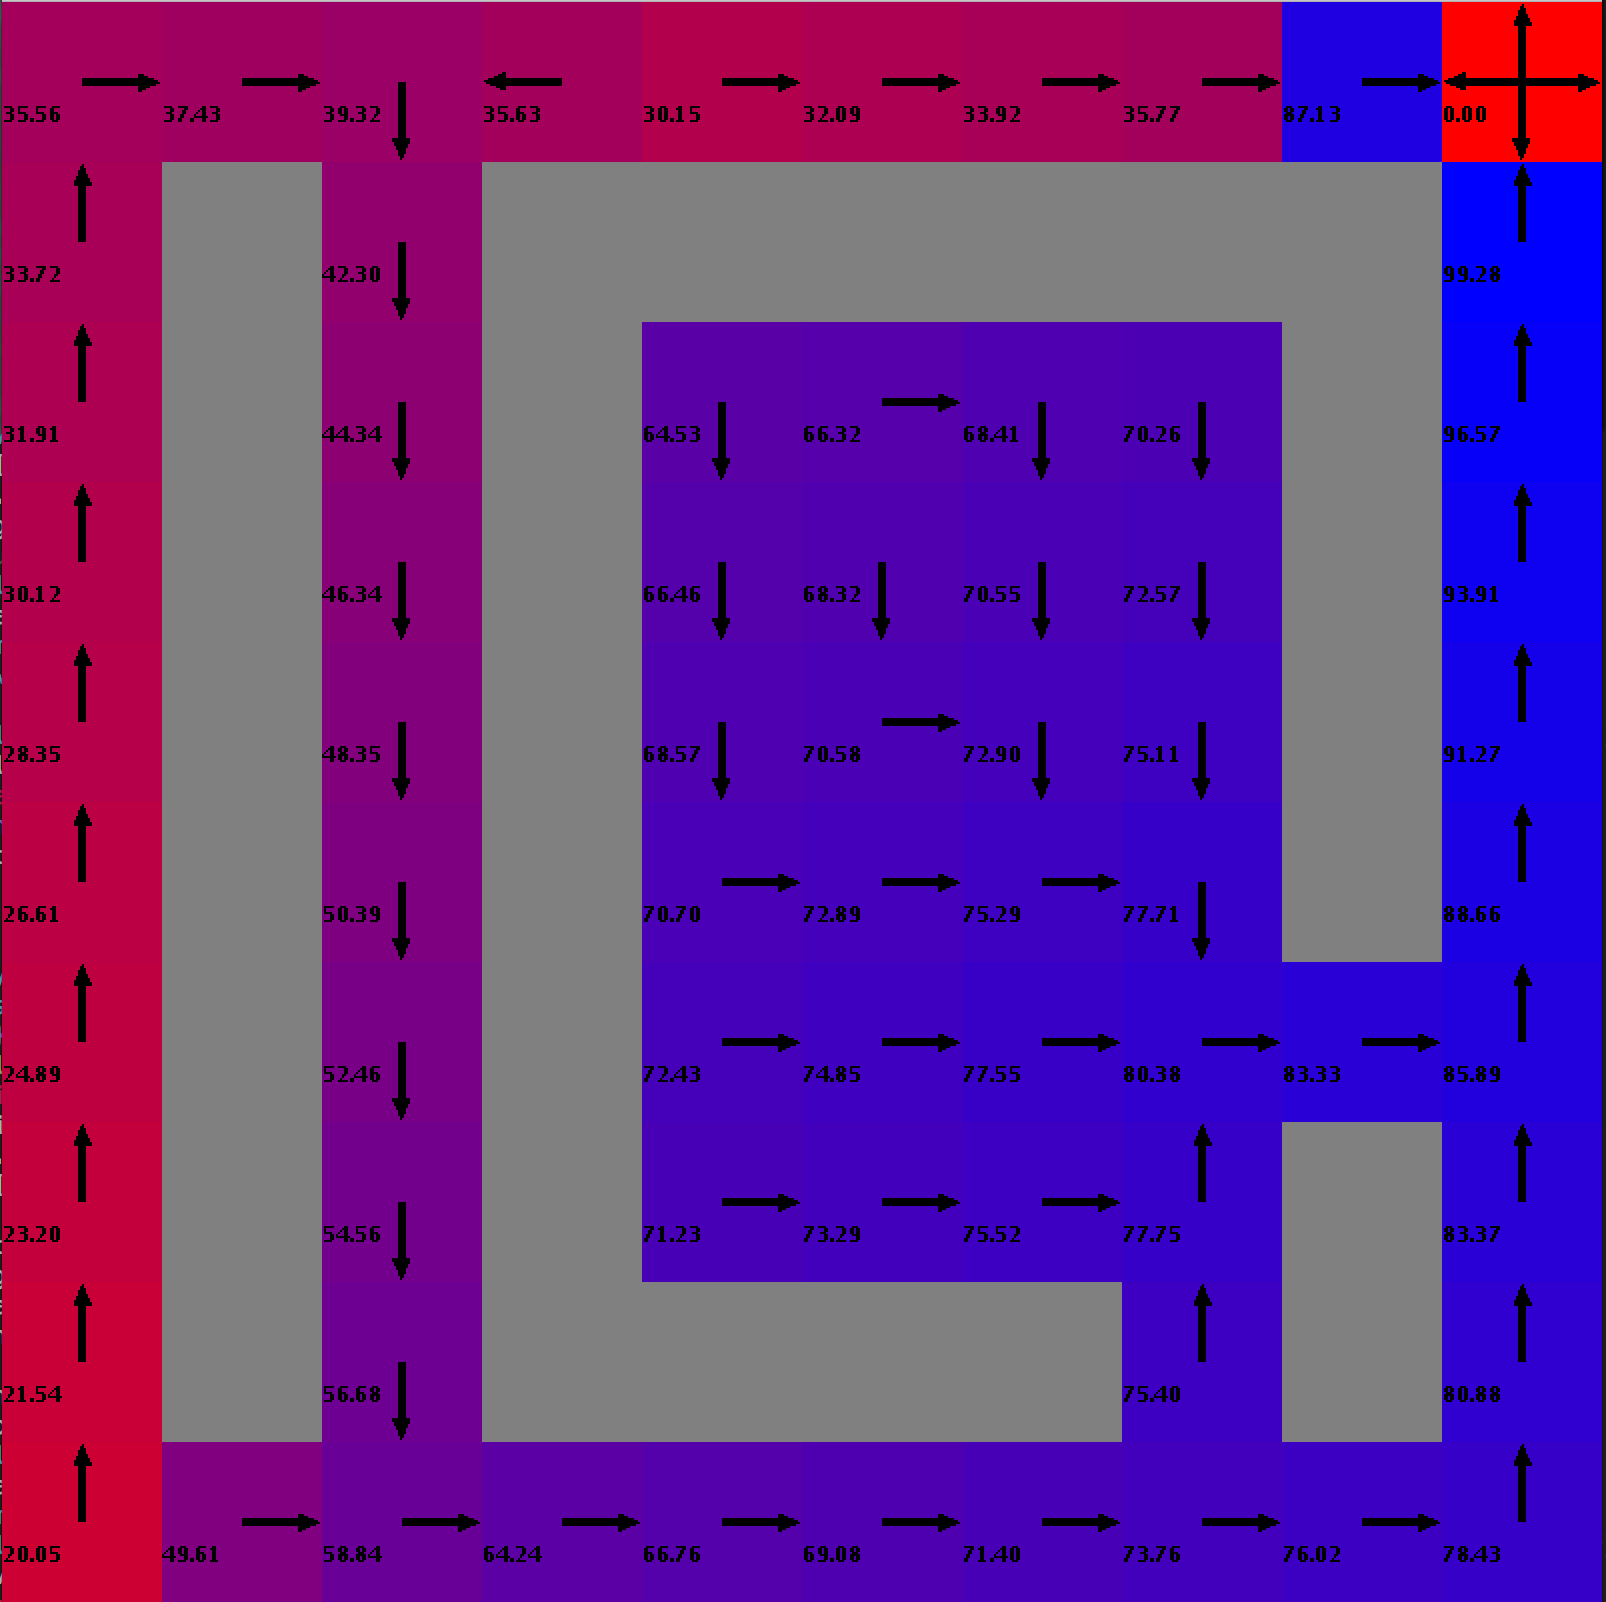
\includegraphics[width=1\textwidth,keepaspectratio]{easy-value-64.png} 
      \caption*{Easy GW Value Iteration \#64} 
   \endminipage\hfill
   \minipage{0.32\textwidth}
      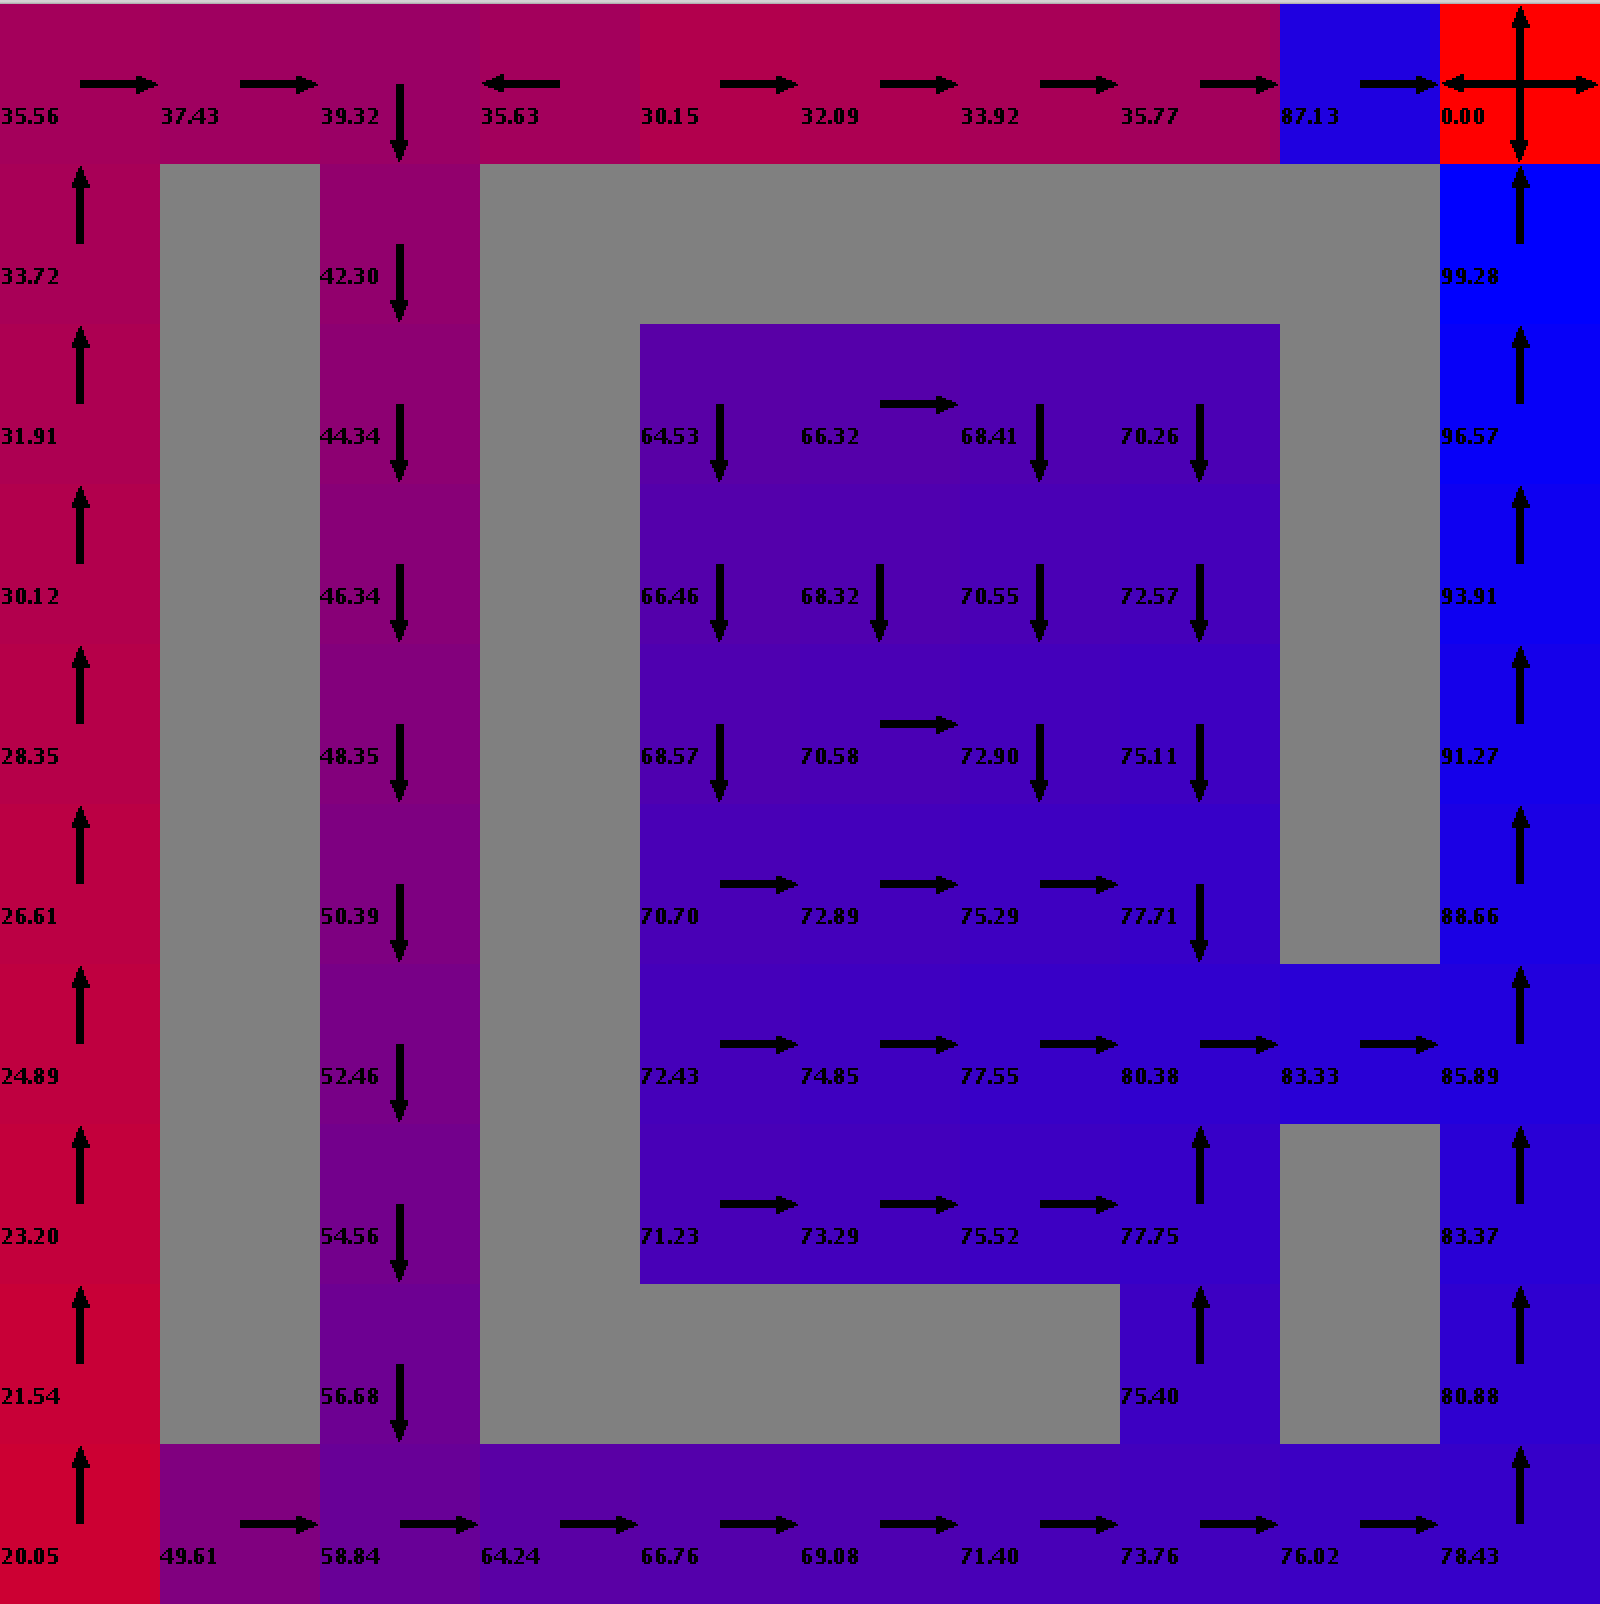
\includegraphics[width=1\textwidth,keepaspectratio]{easy-policy-33.png} 
      \caption*{Easy GW Policy Iteration \#33} 
   \endminipage\hfill
   \minipage{0.32\textwidth}
      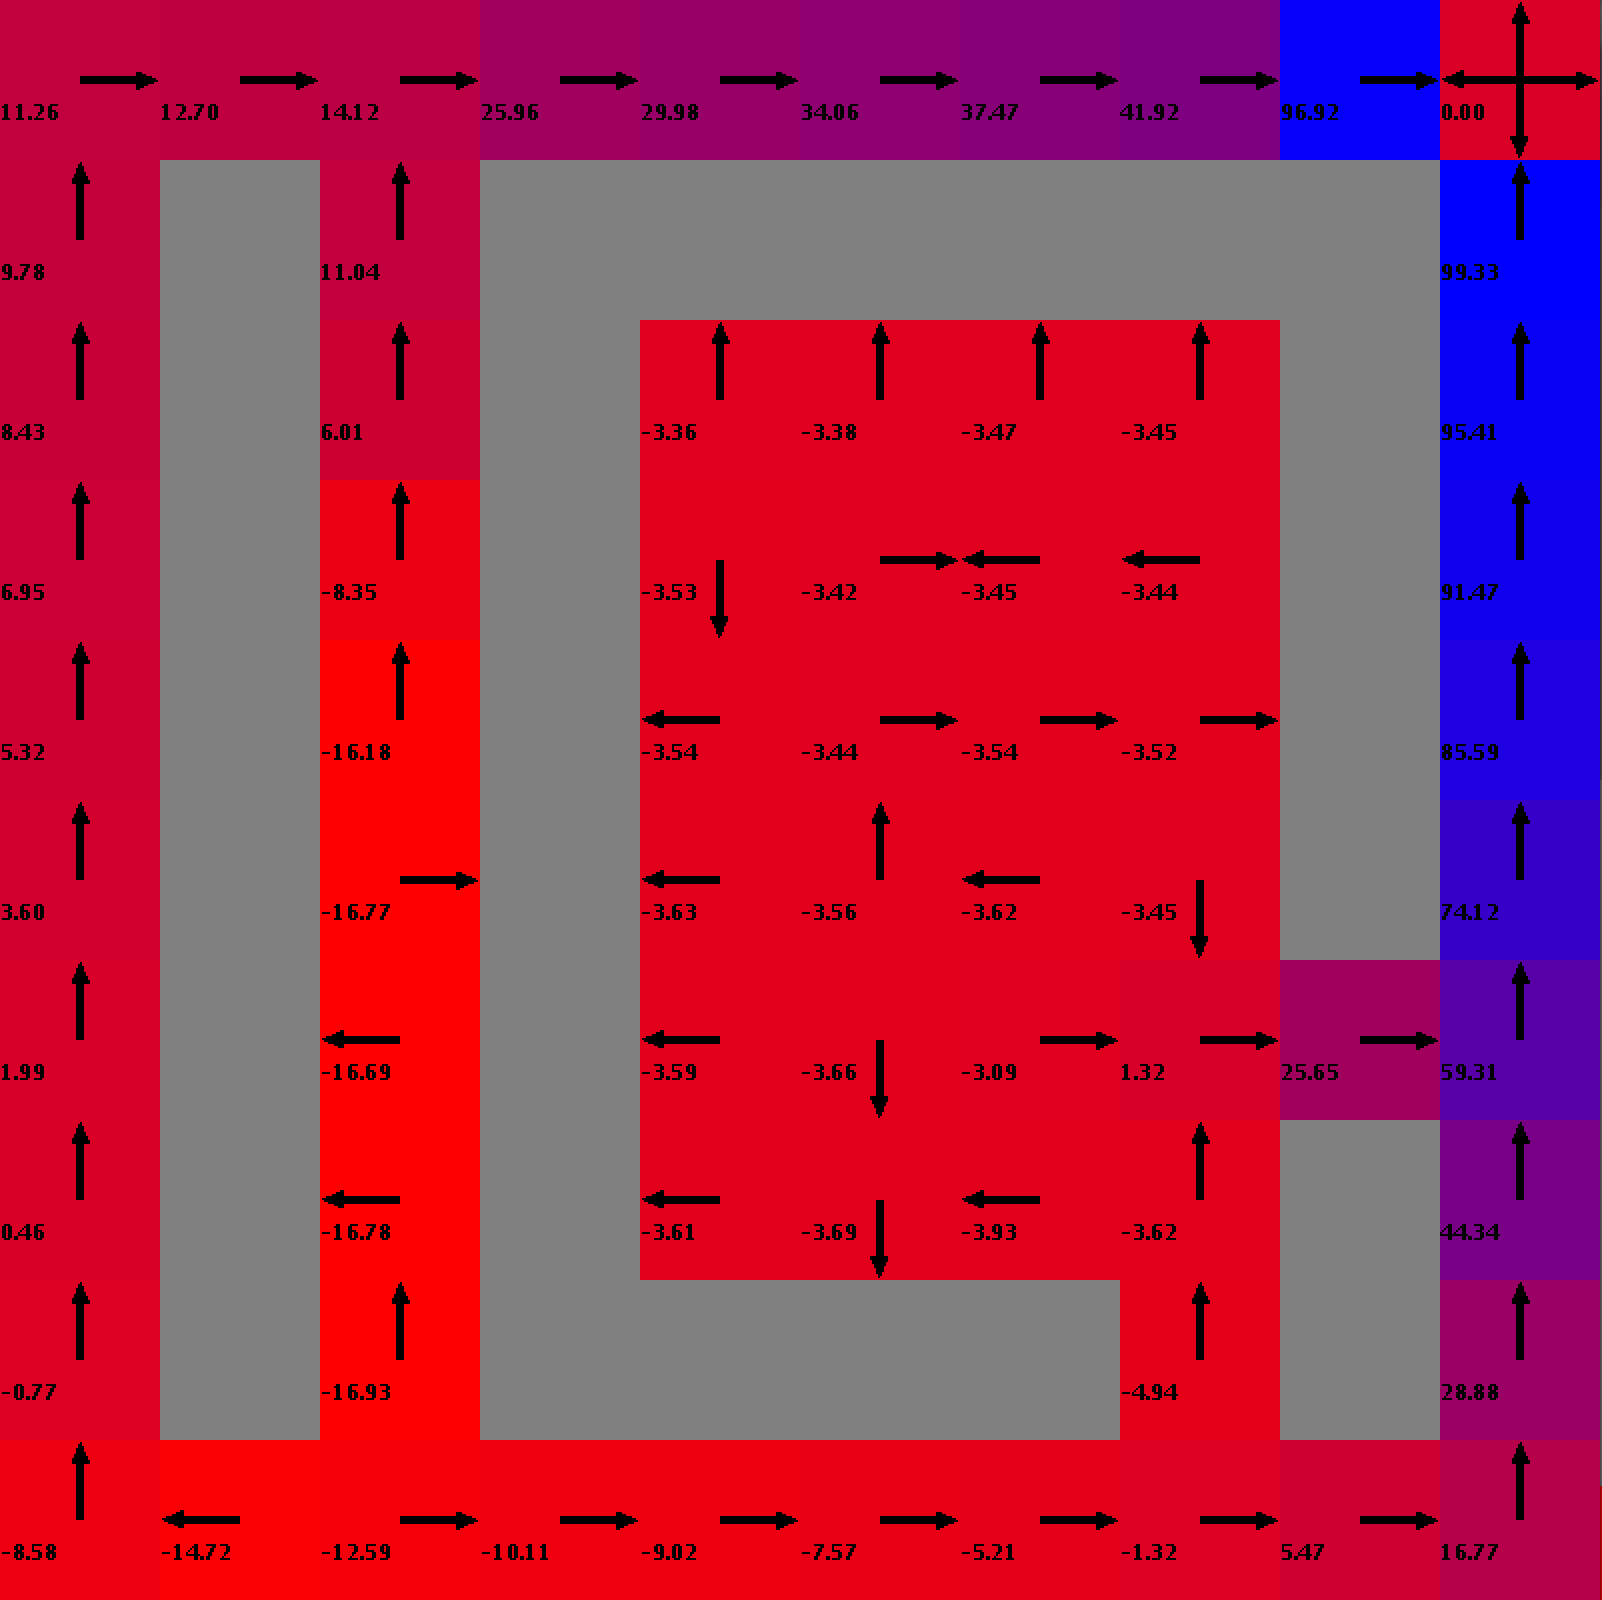
\includegraphics[width=1\textwidth,keepaspectratio]{easy-q-1000.png} 
      \caption*{Easy GW Q-Learning Iteration \#1000} 
   \endminipage\hfill
\end{figure}

  \begin{figure}[H]
   \minipage{0.32\textwidth}
      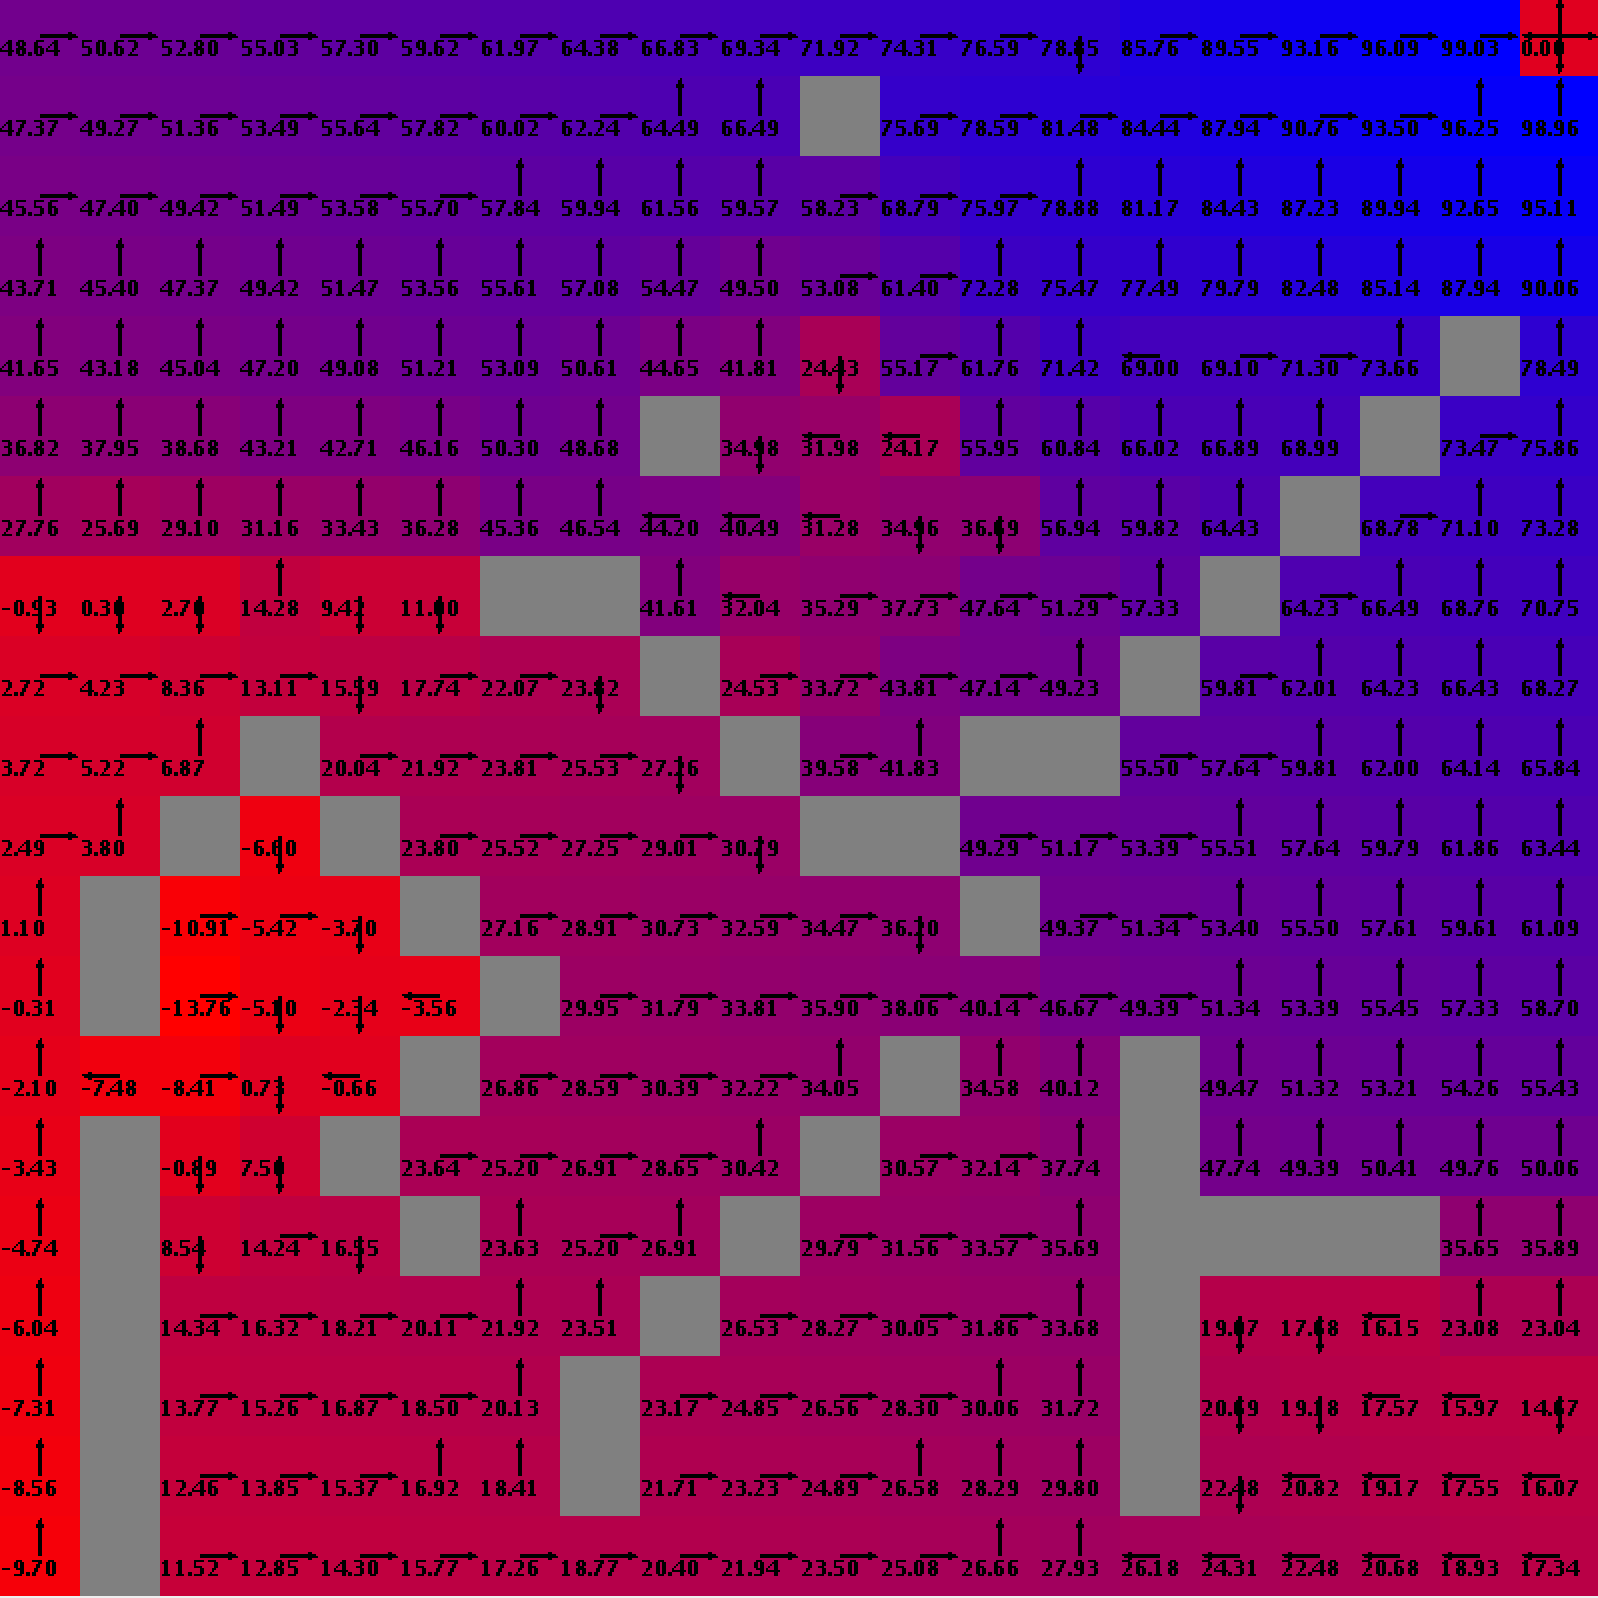
\includegraphics[width=1\textwidth,keepaspectratio]{hard-value-61.png} 
      \caption*{Hard GW Value Iteration \#61} 
   \endminipage\hfill
   \minipage{0.32\textwidth}
      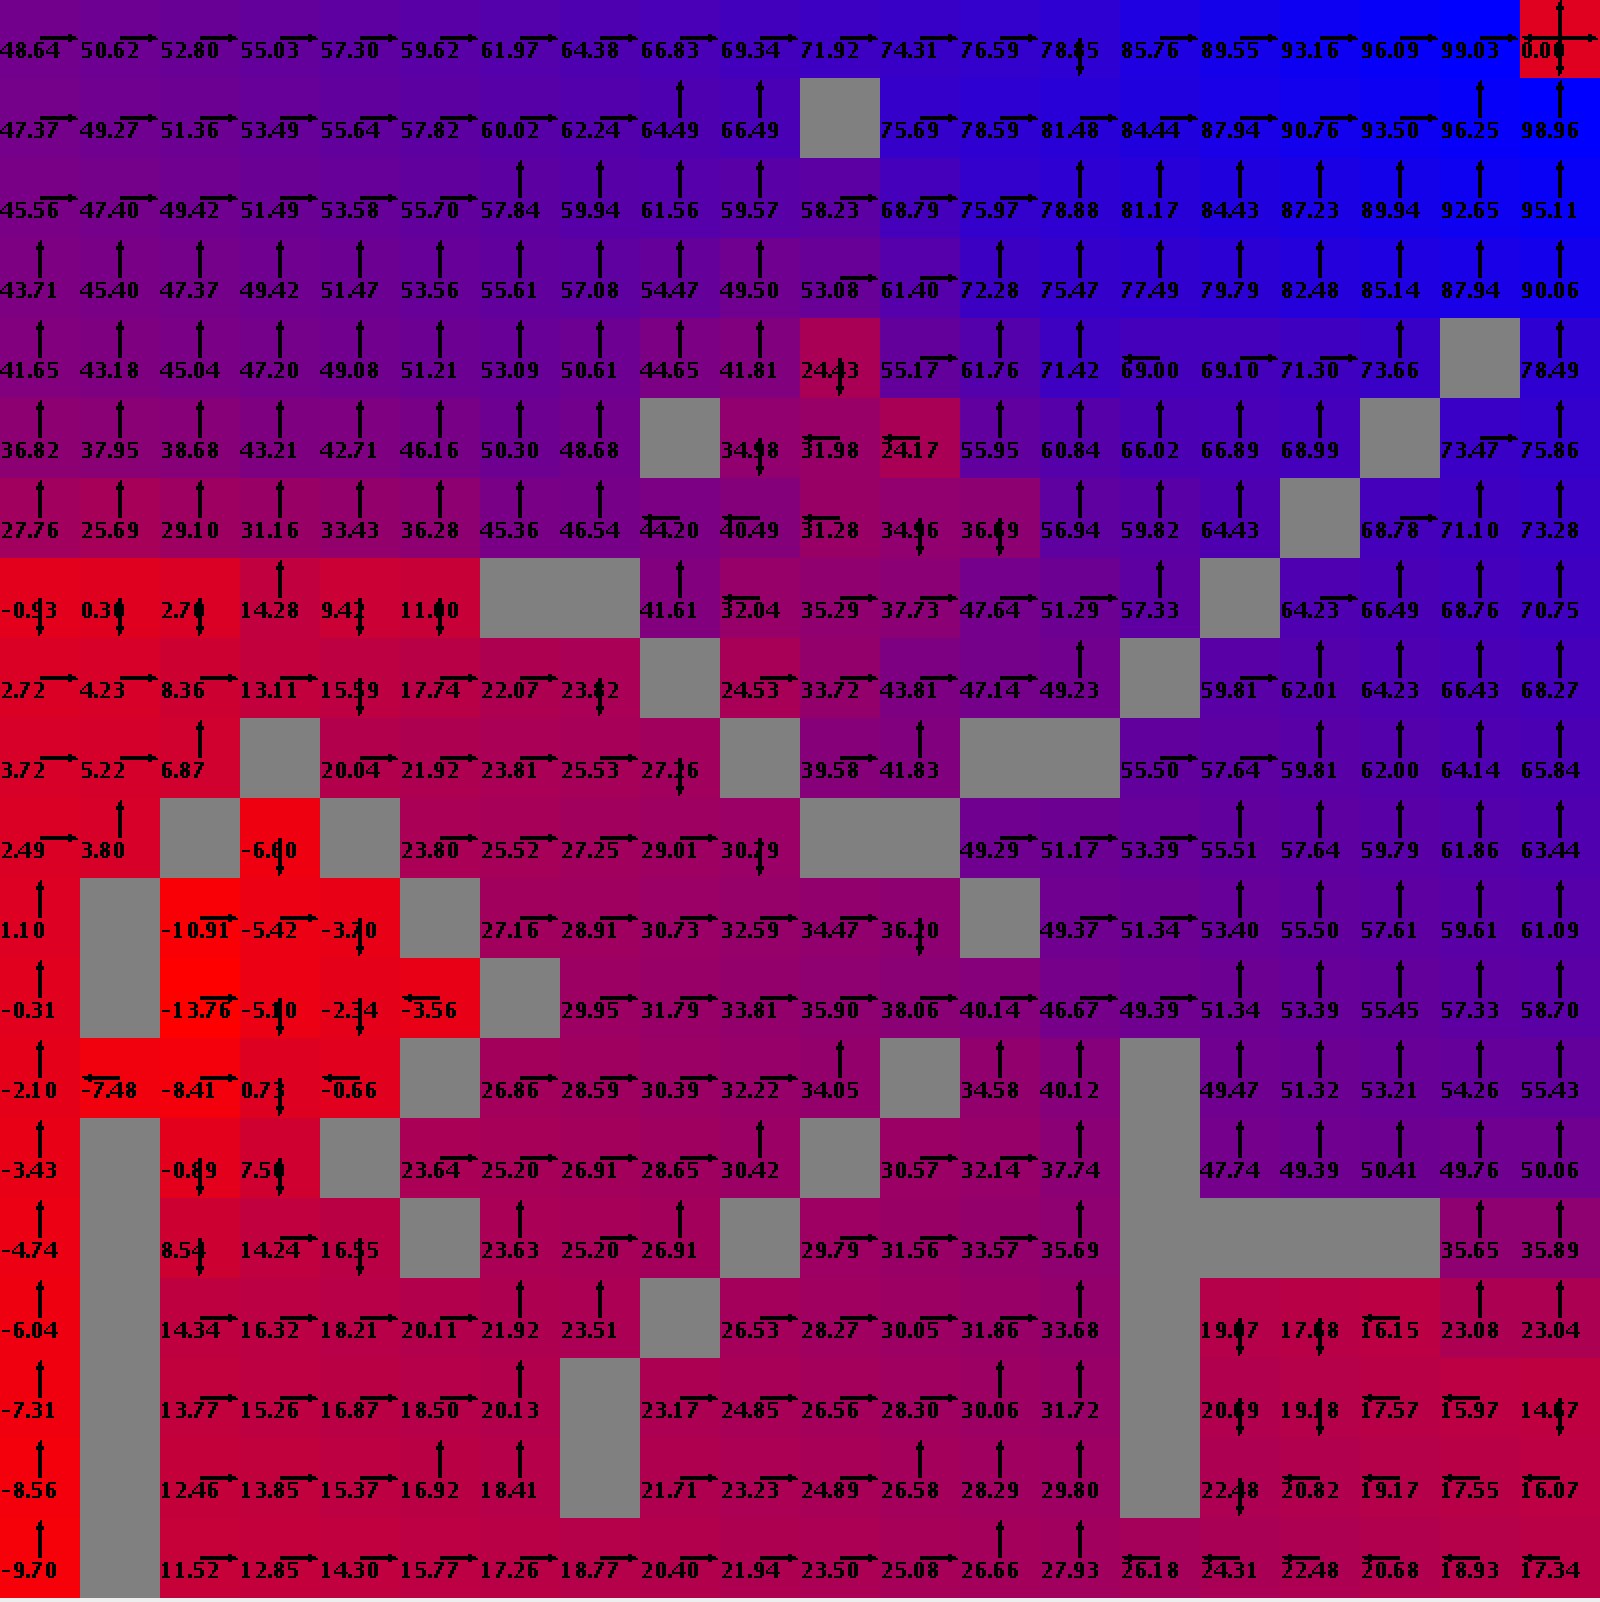
\includegraphics[width=1\textwidth,keepaspectratio]{hard-policy-22.png} 
      \caption*{Hard GW Policy Iteration \#22} 
   \endminipage\hfill
   \minipage{0.32\textwidth}
      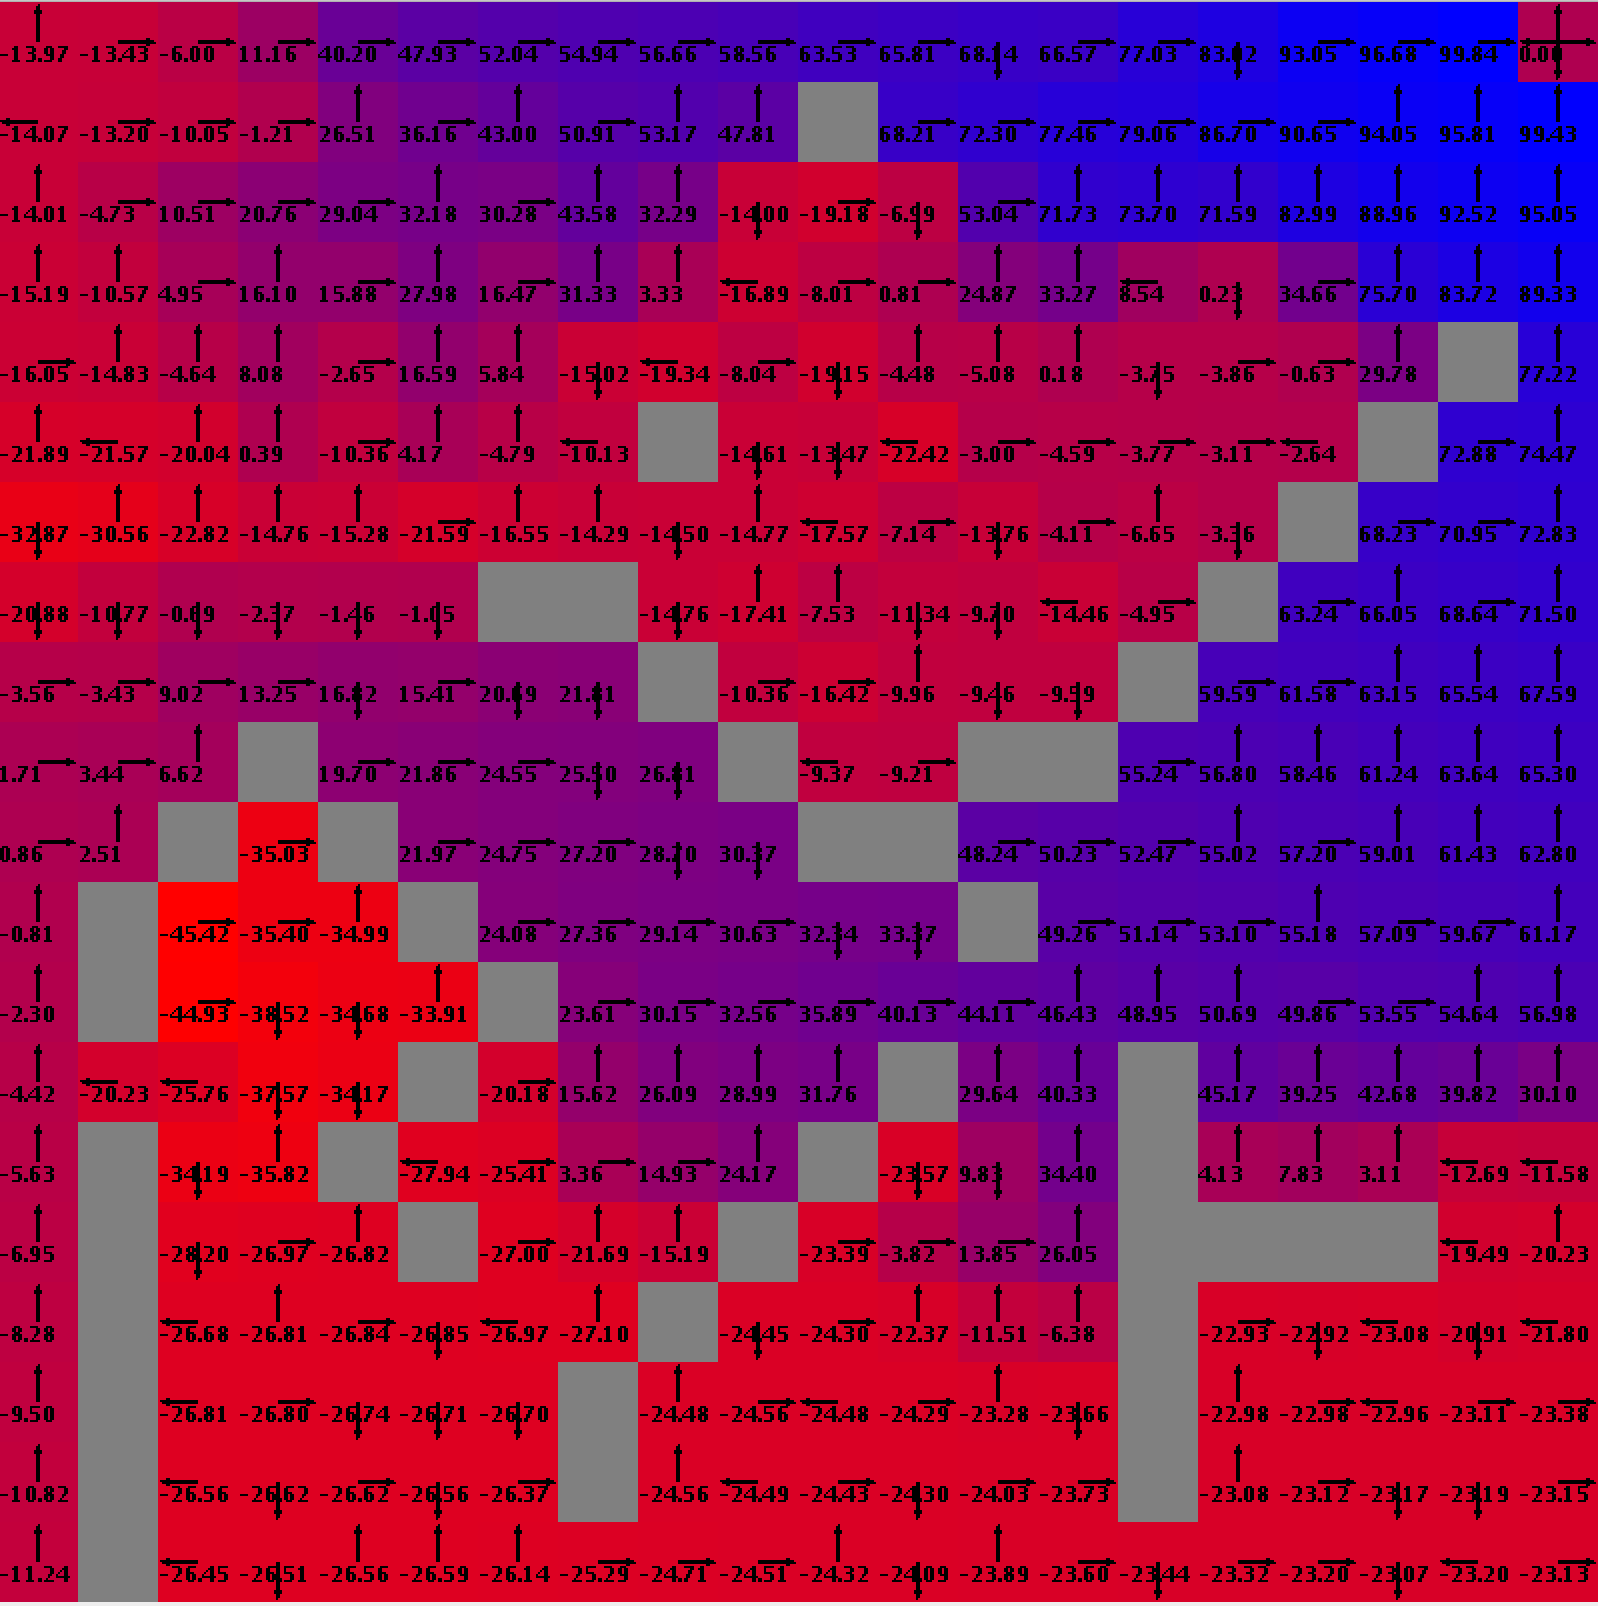
\includegraphics[width=1\textwidth,keepaspectratio]{hard-q-2900.png} 
      \caption*{Hard GW Q-Learning Iteration \#2900} 
   \endminipage\hfill
\end{figure}

\section*{Conclusion}
In this analaysis, two Markov Decision Processes were proposed, disected, and then solved using three different reinforcement learning algorithms: 
value iteration, policy iteration, and Q-learning.  The different algorithms were compared and contrasted, to arrive at various conditions where one may be more optimal than
others.
\\ \\
While Q-learning tends to take many iterations 
to converge, value and policy iteration do so in much fewer iterations.  Interestingly though, in terms of raw time q-learning is instead much quicker.  
In the event that the model is known beforehand, value and policy iteration tend to 
be able to compute the optimal policy much more aptly.  In the event that no model 
is known, Q-learning is able to handle the situation better due to its ability to 
explore and discover as it iterates.  


\end{document}